\documentclass[12pt,letterpaper,twoside,openany]{book}
\usepackage[top=2cm, bottom=2cm, lmargin=4cm,rmargin=2cm,marginparwidth=6cm,marginparsep=2em]{geometry} 
\reversemarginpar
\usepackage{import}
\usepackage{chapter-section-design}
\usepackage{preamble}

 
\usepackage{makeidx}
\makeindex
 
\begin{document}
 
\frontmatter
% \noindent\makebox[\textwidth]{\rule{\textwidth}{0.4pt}}

% \huge{Math 255}

% \noindent\makebox[\textwidth]{\rule{\textwidth}{0.4pt}}

\begin{titlepage} % Suppresses headers and footers on the title page

	\centering % Centre everything on the title page
	
	\scshape % Use small caps for all text on the title page
	
	\vspace*{\baselineskip} % White space at the top of the page
	
	%------------------------------------------------
	%	Title
	%------------------------------------------------
	
	\rule{\textwidth}{1.6pt}\vspace*{-\baselineskip}\vspace*{2pt} % Thick horizontal rule
	\rule{\textwidth}{0.4pt} % Thin horizontal rule
	
	\vspace{\baselineskip} % Whitespace above the title
	
	{\LARGE Applied Mathematics for Chemists II} % Title
	
	\vspace{0.3\baselineskip} % Whitespace below the title
	
	\rule{\textwidth}{0.4pt}\vspace*{-\baselineskip}\vspace{3.2pt} % Thin horizontal rule
	\rule{\textwidth}{1.6pt} % Thick horizontal rule
	
	\vspace{2\baselineskip} % Whitespace after the title block
	
	%------------------------------------------------
	%	Subtitle
	%------------------------------------------------
	
	Vector fields, partial differentiation, cylindrical and spherical coordinates, multiple integrals, line integrals, the wave and the Schr\"odinger equations, separation of variables method. Inner Product Spaces. Fourier Series. % Subtitle or further description
	
	\vspace*{3\baselineskip} % Whitespace under the subtitle
	
	%------------------------------------------------
	%	Editor(s)
	%------------------------------------------------
	
	By
	
	\vspace{0.5\baselineskip} % Whitespace before the editors
	
	{\scshape\Large Colin Roberts \\} % Editor list
	
	\vspace{0.5\baselineskip} % Whitespace below the editor list
	
	\textit{Colorado State University} % Editor affiliation
	
	\vfill % Whitespace between editor names and publisher logo
	
	%------------------------------------------------
	%	Publisher
	%------------------------------------------------
	
	%\plogo % Publisher logo
	\begin{figure}[H]
	    \centering
	    
\includegraphics[width=.8\textwidth]{Frontmatter/ram_logo.jpg}
	\end{figure}
	
	\vspace{0.3\baselineskip} % Whitespace under the publisher logo
	
	Created in Spring 2020\\
    Updated in Spring 2021 % Publication year
	
% 	{\large publisher} % Publisher

\end{titlepage}

\section*{Preface}

This text was created to be a companion to the Math 255 - \emph{Calculus for Biological Students II} course at Colorado State University.  The reader is expected to have completed the Math 155 course with a solid grasp of the material in order for one to best absorb new topics in this course.

The aim of this text is to present relevant topics in \emph{multivariate calculus} and \emph{differential equations}.  To begin, one must learn some \emph{linear algebra}. Linear algebra provides a foundation that is required for studying functions of more than one variable.  It is also an extremely beautiful and applicable field of mathematics itself.  Vectors will serve as a generalization of the system of numbers one is already comfortable with.  With vectors, one can study systems that are naturally living in space.  We are already familiar with how functions can be applied to the real numbers, but they can also be applied to vectors living in space.  The simplest types of vector-functions are those that are \emph{linear}.  Given the simplicity, we often wish to understand more complicated functions by investigating their linear approximations.

Calculus studies the rate of change of functions, but it can be rephrased slightly.  Rather, we take the approach that calculus investigates the best linear approximations to functions.  With one variable, a function can be approximated by a tangent line with a slope found by computing the derivative. This is the best linear approximation to a function of one variable.  When functions input and output more than one variable, the derivative is thus a linear function. This slight rewording of the derivative definition allows for the analysis of functions defined in space and time much more naturally.  Of course, we also care about integration. Integration of functions with more than one variable allows for more types of integration.  That is, we can consider integration as a tool to find lengths of curves, areas, volumes, and other physically meaningful quantities.  

Many systems are easier to understand by studying how they change.  For example, if we push an object it accelerates; acceleration is the second derivative of the position function of an object.  In this case, the system is determined by rates of change and so the equation one writes down for this system is a differential equation.  To model systems that change over space and time, one must be able to write down and solve these differential equations.  Physical intuition can help guide one to a solution, but there are more surefire methods.  The main technique proposed is to simplify the problem just enough so that we can solve it more easily but not lose too much information.  Techniques from linear algebra continue to reemerge and allow us to solve a large class of (linear/first order) problems.  Other (nonlinear/higher order) problems can be simplified down to the case we work to solve.  Thus, we create quite a toolbox to investigate differential systems.


 
\clearpage
\thispagestyle{empty}
 
\tableofcontents
 
\mainmatter
% \chapter{Introduction}
% In 1980, Alberto Calder\'on proposed an inverse problem in his paper \emph{On an inverse boundary value problem} \cite{calderon_inverse_2006} where he asks if one can determine the electrical conductivity matrix of some Ohmic medium from knowledge of voltage and current measurements on the boundary of the given domain. This problem goes under the name of Electrical Impedance Tomography (EIT). Physically, the EIT problem is a static 3-dimensional boundary value inverse problem wherein the practicioner has access to voltage to a discrete subset of the boundary of a body and make noisy measurements of the outgoing current flux along the same discrete subset. In other words, a partial and noisy version of the voltage-to-current map is known.

One notes that the voltage-to-current map inputs a scalar potential (the Dirichlet data) on the boundary which, if the conductivity matrix was known, would allow one to determine the potential on the interior by solving a second order elliptic partial differential equation with coefficients defined by the conductivity. In an Ohmic material, the current field is induced by from the electric field (the gradient of the potential) and the conductivity, and hence for a fixed conductivity, utilizing different Dirichlet data can induce different current fields in the body. The practicioner has the ability to measure the outgoing current flux along the boundary (the Neumann data) and thus, they have access to the voltage-to-current map.   

This problem can be generalized naturally into dimensions $\geq 2$ as a geometric inverse problem. One replaces the medium with a manifold and the conductivity becomes the Riemannian metric. Thus, the second order elliptic equation from before amounts to finding scalar fields in the kernel of the Laplace-Beltrami operator. This leads to a small caveat that in dimension 2 since the Laplace-Beltrami operator is conformally invariant. At any rate, the EIT problem is equivalent to determining an unknown Riemannian manifold up to isometry from the classical Dirichlet-to-Neumann (DN) map which inputs a scalar field and outputs the outward normal component of the derivative of the solution \cite{feldman_calderproblem_nodate, salo_calderon_nodate, uhlmann_inverse_2014}. 

There are a handful of approaches to solving this problem, but it remains unsolved. In order to make progress, theorists have allowed themselves access to larger sets of data, for example, complete knowledge of a generalized DN map on differential forms \cite{krupchyk_inverse_2011,sharafutdinov_complete_2013,belishev_dirichlet_2008,joshi_inverse_nodate}. In dimension 2, the smooth problem has been solved up to conformal invariance and in dimension $\geq 3$, the problem has been solved for analytic manifolds \cite{lassas_determining_2001}. Another approach that is unique to a manifold of dimension 2 appears in \cite{belishev_calderon_2003}. In this paper, Belishev determines the algebra of holomorphic functions from the DN map and realizes the spectrum of this algebra homeomorphic to the underlying manifold by Gelfand. The metric $g$ is then recovered up to conformal class by extracting the complex structure from this algebra as well. An attempt to generalize this approach to dimension $n=3$ can be found in by replacing the complex structure with a quaternionic structure but this has not lead to a complete solution \cite{belishev_algebras_2017, belishev_algebraic_2019}. It has been shown that the 3-dimensional round ball can be determined up to homeomorphism from a quaternionic spectrum. Belishev and Vakulenko ask whether this can be extended to higher dimensions and to other spaces. An answer to this question is provided by \cref{thm:gelfand}.

In this work, I first introduce the geometric algebras $\G$ as special cases of more general Clifford algebras in \cref{subsec:clifford_and_geometric_algebras}. Following this, I take a smooth, oriented, Riemannian manifold $M$ and construct a Clifford algebra bundle whose sections lie in the space $\G(M)$ and are referred to as multivector fields in \cref{sec:geometric_manifolds}. The graded algebraic structure of $\G(M)$ expands upon the exterior algebra of forms $\Omega(M)$, and moreover, there exists a natural differential structure via the gradient operator $\grad$, which finds similarities to the Hodge-Dirac operator $d+\delta$. The space $\G(M)$ proves to be more rich than $\Omega(M)$ since one can realize $\Omega(M)$ as a trivial case of some $\G(M)$. Moreover, it is quite natural to look at multivector fields that consist of many differently graded elements at once. For example, multivector fields that lie in the kernel of $\grad$ are called monogenic and these fields share many of the same properties as holomorphic functions on $\C$ including, but not limited to, a Cauchy integral formula \cref{eq:cauchy_integral}. However, unlike holomorphic functions, the space of monogenic fields $\monogenicfields{}$ is not, in general, commutative or an algebra.

A useful version of a Green's formula is shown in \cref{thm:multivector_greens_formula}, and this allows us to prove a multivector version of the Hodge-Morrey decomposition that we realize in the following theorem.
\begin{customthm}{3.1.1}[Monogenic Hodge Decomposition]
The space of multivector fields $\G(M)$ has the $L^2$-orthogonal decomposition
\begin{equation}
\G(M) = \monogenicfields{} \oplus \pseudoscalar^{-1} \grad \G(M).
\end{equation}
\end{customthm}

The space $\monogenicfields{}$ is a right module over the constant multivectors $\G$. For the special case of the Euclidean geometric algebra $\G_n$, I define a space of module homomorphisms from $\monogenicfields{}$ to $\G_n$ and refer to these morphisms $\G_n$-functionals. Inside $\monogenicfields{}$ lie commutative subalgebras $\algebra{\bivector}(M)$ that are analogs of $\C$ and on these algebras we can define $\G_n$-characters as the $\G_n$-functionals that are also algebra morphisms on each $\algebra{\bivector}(M)$ into $\G_n$. The space of $\G_n$-characters, $\characters(M)$, with the weak-$\ast$ topology, is shown to be homeomorphic to $M$ in the special case where $M$ is a region of $\R^n$ and inherits the Euclidean metric. This is summarized in the following theorem.
\begin{customthm}{3.3.1}
For any $\delta \in \characters(M)$, there is a point $x^\delta \in M$ such that $\delta(f) = f(x^\delta)$ for any $f\in \monogenics(M)$ a monogenic field. Given the weak-$\ast$ topology on $\dualmonogenics(M)$, the map
\[
\gamma \colon \characters(M) \to M, \quad \delta \mapsto x^\delta
\]
is a homeomorphism. 
%The Gelfand transform 
%\[
%\widehat{~} \colon \monogenics(M) \to C(\characters(M); \G_n), \quad \widehat{f}(\delta) \coloneqq \delta(f), \quad \delta \in \characters(M),
%\]
%is an isometry onto its image, so that $\characters(M)$ is isomorphic to $\widehat{\monogenics(M)}$ as algebras.
\end{customthm}

Owing to the original intention of this work, I consider physical and geometric inverse boundary value problems related to the Calder\'on problem. For example, I discuss the electric and magnetic impedance tomography problems and their statements in terms of multivector fields \cref{sec:tomography}. Relationships between the two problems are established, and one finds that the Ohmic property of a medium couples together the scalar potential $u$ and the magnetic bivector field $b$ into a single monogenic field. Given knowledge of the electrostatic and magnetostatic version of the DN map alongside this new relationship, can one determine the underlying conductivity? Likewise, in higher dimensions, do \cref{thm:gelfand,thm:monogenic_hodge} provide new tools for solving the Calder\'on or other related inverse problems? Finally, there also exists a Hilbert transform in two guises via \cite{belishev_dirichlet_2008,brackx_hilbert_2008}. Are these two notions equivalent? Does either add any more useful information for solving boundary inverse problems?

\chapter{Tutorials}
\section{Wolfram Alpha}
Wolfram Alpha (WA) is an online tool that can perform many useful tasks.  Essentially every problem posed in this text could be done using WA.  It is therefore worthwhile to learn some basic input.  Of course, much more can be done with WA than is presented here.  

\subsection{Solving Algebraic Expressions}
An algebraic expression is an equation where one wishes to find a value for a variable (resp. variables) which make the equality in the equation (resp. equations) hold.  

\begin{ex}{One Variable Algebraic Expression}{one_variable_expression}
Consider the equation
\[
3x^4+2x^3+x-5=0.
\]
The goal is to find the value of $x$ so that the left hand side is equal to zero.  There is a formula like the quadratic formula one can use to solve this, but it is rather ugly (see: quartic formula). So, it is rather appealing to use technology to quickly solve this for us.

In the WA entry box, type

\begin{center}
\begin{BVerbatim}
    3x^4+2x^3+x-5=0
\end{BVerbatim}
\end{center}

and press enter.  Give the computation some time, and verify that you find the following solutions:
\begin{align*}
    x &\approx -1.4176\\
    x &\approx 0.94346\\
    x &\approx 0.09627 - 1.11216 i\\
    x &\approx 0.09627 + 1.11216 i.
\end{align*}
\end{ex}

If we have multiple variables, we can perform a similar computation.  

\begin{ex}{Multivarialbe Algebraic Expressions}{multivariable_alg_exp}
Consider the equations
\begin{align*}
    xyz&=1;\\
    x+y&=2;\\
    y+z&=1/2.
\end{align*}
The goal is to find values for $x$, $y$, and $z$ so that each equation is satisfied simultaneously.  These equations can take time to solve and can be prone to errors.  In the WA entry box, type

\begin{center}
    \begin{BVerbatim}
    xyz=1; x+y=2; y+z=1/2
    \end{BVerbatim}
\end{center}

and press enter.  Once the computation has completed, verify that you find the following solutions
\begin{align*}
    x\approx-0.253156,\quad y\approx2.25316,\quad z\approx-1.75316
\end{align*}
or
\begin{align*}
    x\approx1.87658 - 0.654667 i,\quad y\approx0.123422 + 0.654667 i, z\approx0.376578 - 0.654667 i
\end{align*}
or
\begin{align*}
    x\approx1.87658 + 0.654667 i,\quad y\approx0.123422 - 0.654667 i,\quad z\approx0.376578 + 0.654667 i.
\end{align*}
\end{ex}

\subsection{Error Checking}
There are some issues with the interpreting of input with WA.  For example, WA often thinks certain symbols have implicit relationships.  One case is that it tends to take $y$ and $x$ to be related in that $y(x)$ is a function of $x$.

% D[f(x),{x,n}] derivative operator for wolfram alpha

% matrices and vectors and stuff

\section{Geogebra}

\section{CalcPlot3D}

\part{Linear Algebra}

    \chapter{Vectors}
    \section*{Introduction}
        Often times a single number is not adequate for describing a quantity.  Take for example, velocity.  In order to describe the velocity of a particle, we need to know the direction in space the particle travels along with its speed.  This takes three numbers to describe (since we move in a 3-dimensional space). Compare this to temperature.  At any given point in space, we can describe the temperature with a single number. 
        
        \section{Vectors and Scalars}
        
        We then say the following:
        
        \begin{df}{Scalar}{scalar}
        A \textbf{scalar} \index{scalar} quantity is described by a single number.  
        \end{df}
        
        \begin{df}{Vector}{vector}
        A \textbf{vector} \index{vector} quantity is described by $n$ numbers. 
        \end{df}
        
        We usually represent a vector $\mathbf{v}$ as an arrow starting with a tail at the origin ($\mathbf{0}$), and head at the desired point.  
        
        \begin{center}
        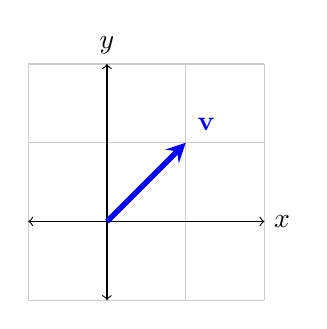
\begin{tikzpicture}
        \draw[thin,gray!40] (-1,-1) grid (2,2);
        \draw[<->] (-1,0)--(2,0) node[right]{$x$};
        \draw[<->] (0,-1)--(0,2) node[above]{$y$};
        \draw[line width=2pt,blue,-stealth](0,0)--(1,1) node[anchor=south west]{$\mathbf{v}$};
        \end{tikzpicture}
        \end{center}
        
        Here in this case we would write $\mathbf{v}=(1,1)$ as the head of the arrow lies where $x=1$ and $y=1$. We should also write, $\mathbf{0}=(0,0)$. More on this notation later.
        
        \begin{ex}{Position of an Object}{position}
        If you are measuring the position of an object $P$ relative to yourself $O$ ($O$ for \emph{origin}), we can describe this with a vector.  We write $\mathbf{p}=\overrightarrow{OP}$ to signify the arrow with the tail at your eyes and head on the object. 
        
        
\begin{center}
\tdplotsetmaincoords{60}{120} 
\begin{tikzpicture} [scale=3, tdplot_main_coords, axis/.style={->,black,thick}, 
vector/.style={-stealth,blue,very thick}, 
vector guide/.style={dashed,red,thick}]

%standard tikz coordinate definition using x, y, z coords
\coordinate (O) at (0,0,0);

%tikz-3dplot coordinate definition using x, y, z coords

\pgfmathsetmacro{\ax}{0.6}
\pgfmathsetmacro{\ay}{1}
\pgfmathsetmacro{\az}{0.8}

\coordinate (P) at (\ax,\ay,\az);

%draw axes
\draw[axis] (0,0,0) -- (1,0,0) node[anchor=north east]{$x$};
\draw[axis] (0,0,0) -- (0,1,0) node[anchor=north west]{$y$};
\draw[axis] (0,0,0) -- (0,0,1) node[anchor=south]{$z$};

%draw a vector from O to P
\draw[vector] (O) -- (P) node[anchor=south east] at (.3,.5,.4){$\mathbf{p}$};

%draw guide lines to components
\draw[vector guide]         (O) -- (\ax,\ay,0);
\draw[vector guide] (\ax,\ay,0) -- (P);
\draw[vector guide]         (P) -- (0,0,\az);
\draw[vector guide] (\ax,\ay,0) -- (0,\ay,0);
\draw[vector guide] (\ax,\ay,0) -- (0,\ay,0);
\draw[vector guide] (\ax,\ay,0) -- (\ax,0,0);
\node[tdplot_main_coords,anchor=east]
at (\ax,0,0){};
\node[tdplot_main_coords,anchor=west]
at (0,\ay,0){};
\node[tdplot_main_coords,anchor=south]
at (0,0,\az){};
\node[tdplot_main_coords, anchor=east] at (0,0,0){$O$};
\node[tdplot_main_coords, anchor=west] at (\ax,\ay,\az){$P$};
\end{tikzpicture}
\end{center}

        If $P$ moves over time, then our vector $\mathbf{p}$ changes over time as well. We'll often denote this $\mathbf{p}(t)$.  It's possible the position of an object changes due to interactions with the environment or other objects.  All to come later.

        \end{ex}
        
        Great, we have some objects, but what can we do with them?  As it turns out, we can do quite a bit.  For the most part, anything we could do with numbers, we can do with vectors.  However, we have to be comfortable looking at things in new ways.
        
        \section{Vector Algebra}
        
        Our first vector operation is \textbf{vector addition}.  Given two vectors $\mathbf{a}$ and $\mathbf{b}$, we can create a new vector
        \[
        \mathbf{c}=\mathbf{a}+\mathbf{b}.
        \]
        Addition is a commutative operation and so we also have that
        \[
        \mathbf{c}=\mathbf{b}+\mathbf{a}.
        \]
        Pictorially, what do we do when we add vectors? We take $\mathbf{a}$ and attach the tail of $\mathbf{b}$ to the head $\mathbf{a}$. 
        
        \begin{center}
        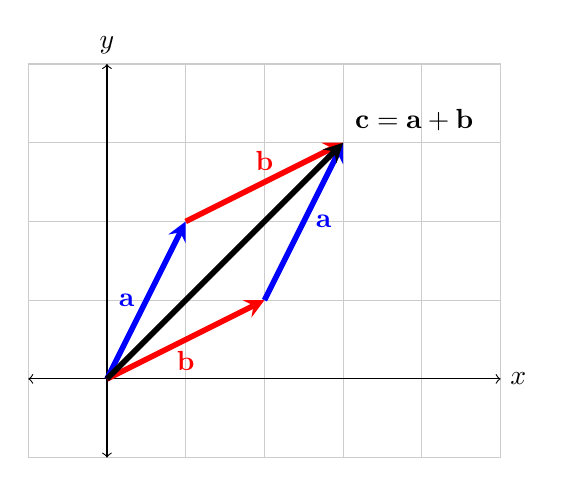
\begin{tikzpicture}
        \draw[thin,gray!40] (-1,-1) grid (5,4);
        \draw[<->] (-1,0)--(5,0) node[right]{$x$};
        \draw[<->] (0,-1)--(0,4) node[above]{$y$};
        \draw[line width=2pt,blue,-stealth](0,0)--(1,2) node[anchor=east] at (.5,1){$\mathbf{a}$};
        \draw[line width=2pt, red, -stealth](0,0)--(2,1) node[anchor=north] at (1,.5){$\mathbf{b}$};
        \draw[line width=2pt, red, -stealth](1,2)--(3,3) node[anchor=south] at (2,2.5){$\mathbf{b}$};
        \draw[line width=2pt, blue, -stealth](2,1)--(3,3) node[anchor=west] at (2.5,2){$\mathbf{a}$};
        \draw[line width=2pt, black, -stealth](0,0)--(3,3) node[anchor=south west]{$\mathbf{c}=\mathbf{a}+\mathbf{b}$};
        \end{tikzpicture}
        \end{center}
        
        From this diagram, you can see why the operation is commutative.  Both paths, $\mathbf{a}+\mathbf{b}$ and $\mathbf{b}+\mathbf{a}$, lead to the same $\mathbf{c}$.
        
        
        As always, repeated addition gives us a form of multiplication. What will this mean here? 
        
        \begin{exercise}
        Draw a 2-dimensional coordinate system ($x$ and $y$ axes), and draw some vector $\mathbf{a}$.  Using vector addition, what does $\mathbf{a}+\mathbf{a}=2\mathbf{a}$ look like? Given this, what do you think $\frac{1}{2}\mathbf{a}$ will look like? 
        \end{exercise}
        
        When dealing with a vector, we are allowed to scale the length.  We call this \textbf{scalar multiplication}. Since the vector $2\mathbf{a}$ has twice the length of $\mathbf{a}$, we would expect $\frac{1}{2} \mathbf{a}$ to have half the length of $\mathbf{a}$.  All of these vectors point in the same direction though.  We have merely scaled their lengths.
        
        \begin{question}
        What happens if we take $-\mathbf{a}$ (i.e., $-1\cdot \mathbf{a}$)? \emph{Hint: Consider what happens for numbers on a number line when multiplied by $-1$.} 
        \end{question}
        
        \begin{answer}
        It flips the direction of the vector.
        \end{answer}
        
        We can take a look at all of this. 
        
        \begin{center}
        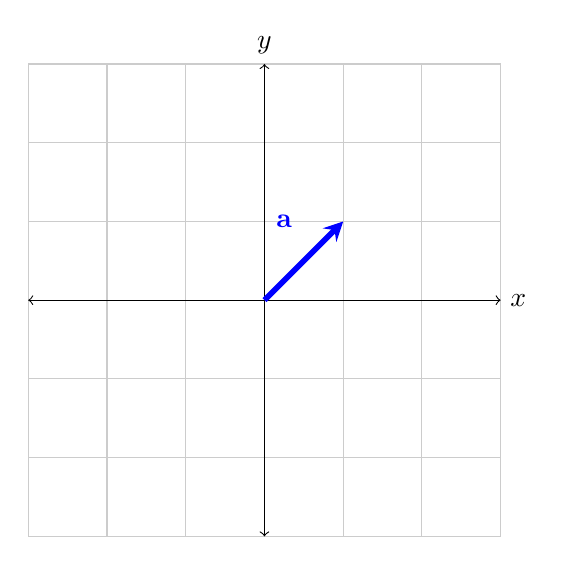
\begin{tikzpicture}
        \draw[thin,gray!40] (-3,-3) grid (3,3);
        \draw[<->] (-3,0)--(3,0) node[right]{$x$};
        \draw[<->] (0,-3)--(0,3) node[above]{$y$};
        \draw[line width=2pt,blue,-stealth](0,0)--(1,1) node[anchor=east] at (.5,1){$\mathbf{a}$};
        \end{tikzpicture}
        \qquad
        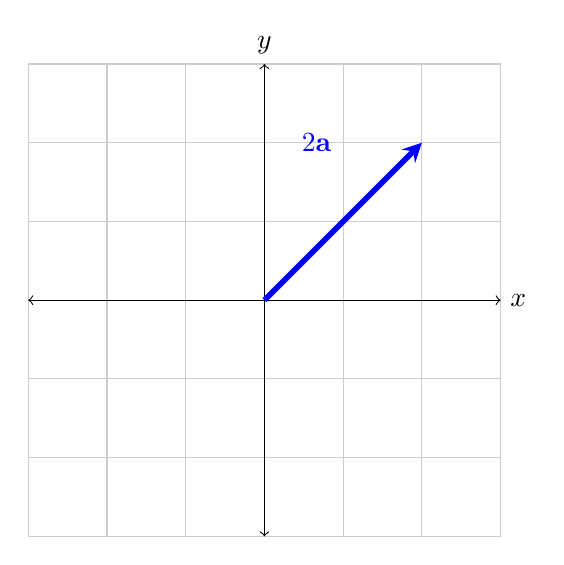
\begin{tikzpicture}
        \draw[thin,gray!40] (-3,-3) grid (3,3);
        \draw[<->] (-3,0)--(3,0) node[right]{$x$};
        \draw[<->] (0,-3)--(0,3) node[above]{$y$};
        \draw[line width=2pt,blue,-stealth](0,0)--(2,2) node[anchor=east] at (1,2){$2\mathbf{a}$};
        \end{tikzpicture}
        
        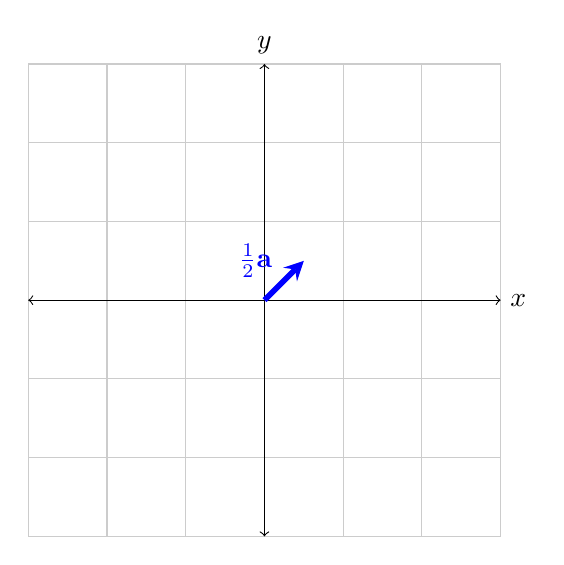
\begin{tikzpicture}
        \draw[thin,gray!40] (-3,-3) grid (3,3);
        \draw[<->] (-3,0)--(3,0) node[right]{$x$};
        \draw[<->] (0,-3)--(0,3) node[above]{$y$};
        \draw[line width=2pt,blue,-stealth](0,0)--(.5,.5) node[anchor=east] at (.25,.5){$\frac{1}{2}\mathbf{a}$};
        \end{tikzpicture}
        \qquad
        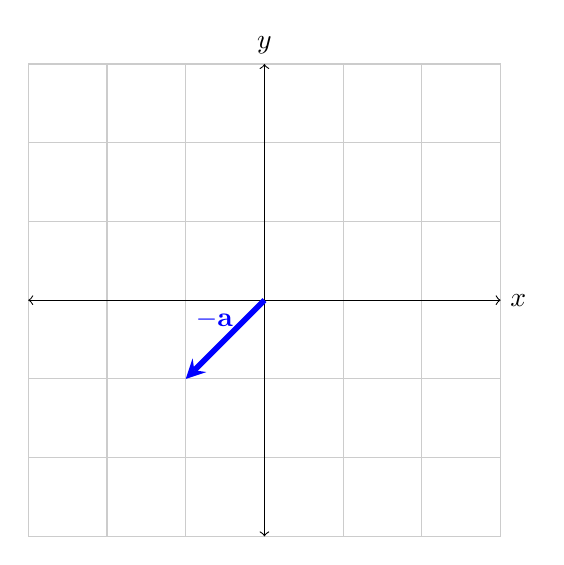
\begin{tikzpicture}
        \draw[thin,gray!40] (-3,-3) grid (3,3);
        \draw[<->] (-3,0)--(3,0) node[right]{$x$};
        \draw[<->] (0,-3)--(0,3) node[above]{$y$};
        \draw[line width=2pt,blue,-stealth](0,0)--(-1,-1) node[anchor=east] at (-.25,-.25){$-\mathbf{a}$};
        \end{tikzpicture}
        \end{center}
        
        \begin{question}
        How can we go about defining $\mathbf{a}-\mathbf{b}$?  
        \end{question}
        
        \begin{answer}
        We can write $\mathbf{a}+(-\mathbf{b})$ and use the rules for vector addition and scalar multiplication together.
        \end{answer}
        
        \begin{exercise}
        Draw two different vectors $\mathbf{a}$ and $\mathbf{b}$ and draw the following:
        \begin{itemize}
            \item $\mathbf{a}+\mathbf{b}$,
            \item $\mathbf{a}-\mathbf{b}$,
            \item $\mathbf{b}-\mathbf{a}$.
        \end{itemize}
        \end{exercise}
        
        Now see the picture below.
        
        \begin{center}
        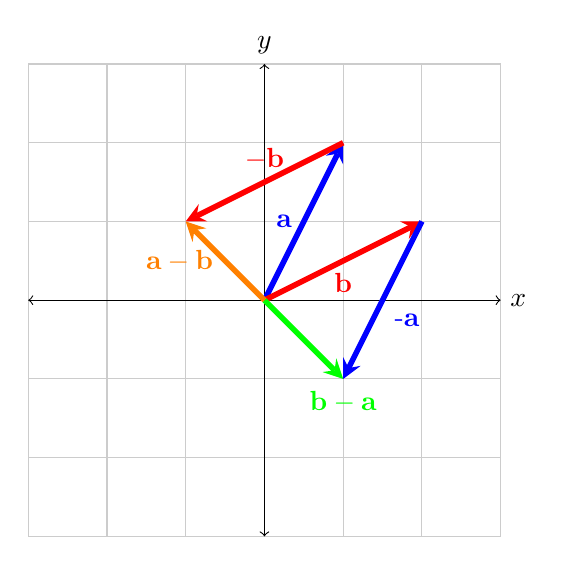
\begin{tikzpicture}
        \draw[thin,gray!40] (-3,-3) grid (3,3);
        \draw[<->] (-3,0)--(3,0) node[right]{$x$};
        \draw[<->] (0,-3)--(0,3) node[above]{$y$};
        \draw[line width=2pt,blue,-stealth](0,0)--(1,2) node[anchor=east] at (.5,1){$\mathbf{a}$};
        \draw[line width=2pt, red, -stealth](0,0)--(2,1) node[anchor=north] at (1,.5){$\mathbf{b}$};
        \draw[line width=2pt, red, -stealth](1,2)--(-1,1) node[anchor=south] at (0,1.5){$-\mathbf{b}$};
        \draw[line width=2pt, blue, -stealth](2,1)--(1,-1) node[anchor=west] at (1.5,-.25){-$\mathbf{a}$};
        \draw[line width=2pt, green, -stealth](0,0)--(1,-1) node[anchor=north]{$\mathbf{b}-\mathbf{a}$};
        \draw[line width=2pt, orange, -stealth](0,0)--(-1,1) node[anchor=east] at (-.5,.5){$\mathbf{a}-\mathbf{b}$};
        \end{tikzpicture}
        \end{center}
        
        
        \section{Vector Components}
        To work with vectors more effectively, it's necessary to break them down into \textbf{components}. Let us consider the following.
        
        \begin{ex}{Components of a Vector}{vector_components}
        Let us fix an arbitrary vector $\mathbf{a}$ in $\R^2$ (i.e., the $xy$-plane).  
        \begin{center}
        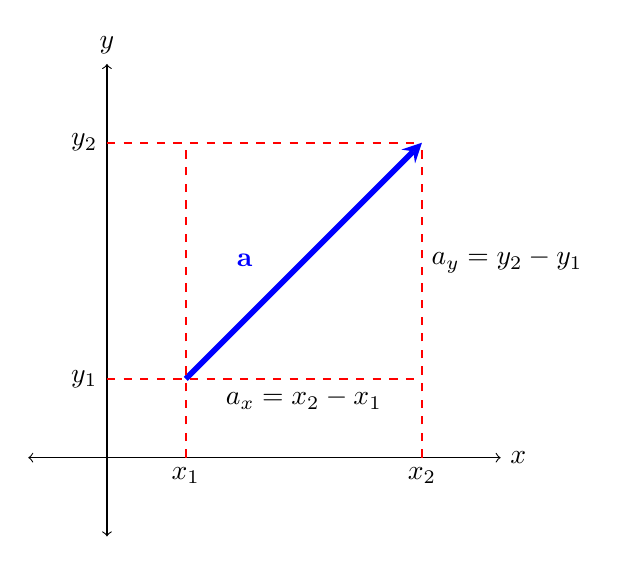
\begin{tikzpicture}[vector guide/.style={dashed,red,thick}]
        \draw[<->] (-1,0)--(5,0) node[right]{$x$};
        \draw[<->] (0,-1)--(0,5) node[above]{$y$};
        \draw[line width=2pt,blue,-stealth](1,1)--(4,4) node[anchor=east] at (2,2.5){$\mathbf{a}$};
        \draw[vector guide] (1,0) -- (1,4);
        \draw[vector guide] (4,0) -- (4,4);
        \draw[vector guide] (0,1) -- (4,1);
        \draw[vector guide] (0,4) -- (4,4);
        \node[anchor=north] at (1,0){$x_1$};
        \node[anchor=north] at (4,0){$x_2$};
        \node[anchor=east] at (0,1){$y_1$};
        \node[anchor=east] at (0,4){$y_2$};
        \node[anchor=north] at (2.5,1){$a_x=x_2-x_1$};
        \node[anchor=west] at (4,2.5){$a_y=y_2-y_1$};
        \end{tikzpicture}
        \end{center}
        We can break down this vector into the portions that are in the $x$-direction and $y$-direction.  We say that the component of the vector in the $x$-direction is $a_x=x_2-x_1$ and the component of the vector in the $y$-direction is $a_y=y_2-y_1$.  It follows that the length of the vector is $|\mathbf{a}|=\sqrt{a_x^2+a_y^2}$ and the direction is the slope $a_y/a_x$. 
        
        We often write vectors in the following way 
        \[
        \mathbf{a}=(a_x,a_y).
        \]
        \end{ex} 
        
        
        \subsubsection{Unit Coordinate Vectors}
        Another way of writing a vector $\mathbf{a}$ is as follows. We create unit vectors $\hat{\mathbf{\i}}=(1,0)$ and $\hat{\mathbf{\j}}=(0,1)$. 
        \begin{center}
        \begin{tikzpicture}[vector guide/.style={dashed,red,thick}]
        \draw[<->] (-1,0)--(3,0) node[right]{$x$};
        \draw[<->] (0,-1)--(0,3) node[above]{$y$};
        \draw[line width=2pt,blue,-stealth](0,0)--(1,0) node[anchor=north] at (1,0){$\mathbf{\hat{\i}}$};
        \draw[line width=2pt, red,-stealth](0,0)--(0,1) node[anchor=east] at (0,1){$\mathbf{\hat{\j}}$};
        \end{tikzpicture}
        \end{center}
        Then another way of writing $\mathbf{a}$ is
        \[
        \mathbf{a}=a_x \mathbf{\hat{\i}}+a_y\mathbf{\hat{\j}}.
        \]

        
        When working in 3-dimensions, we typically use the unit vectors
        \begin{align*}
            \mathbf{\hat{\i}}&=(1,0,0)\\
            \mathbf{\hat{\j}}&=(0,1,0)\\
            \mathbf{\hat{k}}&=(0,0,1).
        \end{align*}
        Sometimes others write
        \begin{align*}
            \mathbf{\hat{\i}}&=\mathbf{\hat{x}}\\
            \mathbf{\hat{\j}}&=\mathbf{\hat{y}}\\
            \mathbf{\hat{k}}&=\mathbf{\hat{z}}.
        \end{align*}

    \section{Vector Algebra with Components}
        It is helpful to think of vectors as an ordered list of numbers. Why? Well, if two ordered lists are to be equal, then each part of the list must also be equal. \begin{enumerate}[(i)]
            \item \textbf{Equality:} Vectors are equal when their components are equal,
            \[
            \mathbf{a}=\mathbf{b} ~~ \textrm{if} ~~ a_x+b_x, ~~ a_y=b_y ~~ \textrm{and} ~~ a_z=b_z.
            \]
            \item \textbf{Addition:} The sum $\mathbf{a}+\mathbf{b}$ is done by adding components together,
            \[
            \mathbf{a}+\mathbf{b}=(a_x+b_x,a_y+b_y,a_z+b_z).
            \]
            \item \textbf{Scalar Multiplication:} The product $\lambda \mathbf{a}$ is obtained by multiplying each component of $\mathbf{a}$ by $\lambda$,
            \[
            \lambda \mathbf{a}=(\lambda a_x,\lambda a_y, \lambda a_z).
            \]
        \end{enumerate}
        
        \begin{exercise} Do the following.  It will really help to draw a picture!
        \begin{enumerate}[(a)] 
            \item Find the vector $\mathbf{a}=\overrightarrow{PQ}$ whose initial point $P$ is $\mathbf{p}=(2,1,0)$ and whose terminal point $Q$ is $\mathbf{q}=(1,3,-2)$.
            \item What is the length of $\mathbf{a}$?
            \item Find the unit vector parallel to $\mathbf{a}$.
        \end{enumerate}
        \end{exercise}
        
        \begin{exercise}
        Given $\mathbf{a}=(2,3,1)$, $\mathbf{b}=(1,-2,0)$, and $\mathbf{c}=(5,2,-1)$, find 
        \begin{enumerate}[(a)]
            \item $\mathbf{d}=2\mathbf{a}+3\mathbf{b}-\mathbf{c}$,
            \item $\|\mathbf{d}\|$ (the length of $\mathbf{d}$),
            \item Let $\lambda$ be a scalar.  Does it make sense to consider $\mathbf{v}=\mathbf{a}+\lambda$? Why or why not?
        \end{enumerate}
        \end{exercise}
        
        \subsubsection{Applications}
        
        \begin{ex}{Center of Mass}{center_of_mass}
        If we have $n$ point masses each with a mass $m_i$ and position $\mathbf{r}_i$, then the center of mass can be written
        \[
        \mathbf{R}_{cm}=\frac{1}{M}(m_1\mathbf{r}_1+m_2 \mathbf{r}_2 + \cdots + m_n \mathbf{r}_n)=\frac{1}{M}\sum_{i=1}^n m_i \mathbf{r}_i
        \]
        where
        \[
        M=\sum_{i=1}^n m_i
        \]
        is the total mass.
        
        The way to think about this is as averaging the position of these particles but keeping track of how much each weighs.  For example, imagine two masses $m_1$ and $m_2$ in one dimension.  If $\mathbf{r}_1=1$ and $\mathbf{r}_2=-1$, then if $m_2>m_1$, the center of mass should be closer to $m_2$ and thus negative.
        \end{ex}
    
        \section{Vector Spaces}
        All of what we have discussed is really leading to the definition of a \textbf{vector space}.  We won't go into vector space theory, but we should at least know the terminology and basic idea.  In the future (say, in a quantum mechanics lecture), you may see functions being treated like vectors.  This is true, but not what we wish to do right now.
        
        \begin{df}{Vector Space}{vector_space}
        A \textbf{vector space} \index{vector!space} $V$ is a collection of vectors that satisfy all the vector algebra properties. Namely,
        \begin{enumerate}[(i)]
            \item There exists a single vector $\mathbf{0}$ such that $|\mathbf{0}|=0.$
            \item We can add any two vectors $\mathbf{u},\mathbf{v}\in V$ to each other so that $\mathbf{u}+\mathbf{v}\in V$ as well. We also have that $\mathbf{0}+\mathbf{v}=\mathbf{v}$ for any $v\in V$.
            \item If we take any $\lambda \in \R$ and $\mathbf{v}\in V$ then $\lambda \mathbf{v} \in V$ as well.
        \end{enumerate}
        \end{df}
        
        The most important vector space for us will be $\R^n$ where $n$ is a positive integer.  $\R^2$ is familiar to us, as it is usually called the $xy$-plane. $\R^3$ is as well, as we usually think of the space surrounding us as being 3-dimensional.
        
        \begin{remark}
        For us, we will always assume that the tail of vectors starts at $\mathbf{0}$ (the origin) unless otherwise stated.  When we get to vector fields, this will be a bit different.
        \end{remark}
        
        \begin{ex}{Examples of Vectors}{examples_of_vecs}
        \begin{itemize}
            \item A vector in $\R^1=\R$ is just a real number.
            \item A vector in $\R^2$ is written as $(x,y)$ or $x\mathbf{\hat{\i}}+y\mathbf{\hat{\j}}$.
            \item A vector in $\R^3$ is written as $(x,y,z)$ or $x\mathbf{\hat{\i}}+y\mathbf{\hat{\j}}+z\mathbf{\hat{k}}$.
            \item A vector in $\R^n$ is written as $(x_1,x_2,\dots,x_n)$ or as 
            $x_1 \mathbf{e}_1+x_2 \mathbf{e}_2+\cdots+x_n \mathbf{e}_n.$ 
        \end{itemize}
        \end{ex}
        We'll soon talk about what the $\mathbf{\hat{\i}}, \mathbf{\hat{\j}}, \mathbf{\hat{k}}, \mathbf{e}_i$ are.
        
        \subsubsection{Linear Combinations}
        If we have a vector space, then we know any scalar multiple of a vector is in this space and addition of any vectors must be as well.  This gives us the notion of a \textbf{linear combination.}
        
        \begin{ex}{Linear Combination}{linear_comb}
        Given two vectors, $\mathbf{v}_1, \mathbf{v}_2$, a linear combination of these two vectors is 
        \[
        \lambda_1 \mathbf{v}_1 + \lambda_2 \mathbf{v}_2.
        \]
        Of course, this extends to as many vectors as we'd like. For example,
        \[
        \lambda_1 \mathbf{v}_1 + \lambda_2 \mathbf{v}_2 + \cdots + \lambda_n \mathbf{v}_n.
        \]
        \end{ex}
        
        This gives us the following idea.  We should be able to decompose any vectors in a vector space into more fundamental components we understand.  We've done this above, but let's make it a bit more formal.
        
        \subsubsection{Basis}
        Given a vector space $V$, we want to find a list of vectors that, by taking a linear combination, can create any vector in $V$.  We call this a \textbf{basis}.
        
        \begin{ex}{Standard Basis}{standard_basis}
        Let $V=\R^n$ and
        \[
        \mathbf{e}_1=(1,0,0,\dots,0) \quad \mathbf{e}_2=(0,1,0,\dots,0) \quad \cdots \quad \mathbf{e}_n=(0,0,0,\dots,1). 
        \]
        Then this collection of $\mathbf{e}_i$ vectors forms a basis for $\R^n$.  
        
        To see this, let's take an arbitrary vector 
        \[
        \mathbf{v}=(v_1,v_2,\dots,v_n).
        \]
        Then, using our basis, we can write
        \[
        \mathbf{v}=v_1 \mathbf{e}_1 + v_2 \mathbf{e}_2 + \cdots + v_n \mathbf{e}_n.
        \]
        
        There are many other bases for $\R^n$, but this will be the one we use for the most part.  We will consider new bases when we talk about eigen-decomposition.
        \end{ex}
        
        \begin{exercise}
        Identify a basis for $\R^2$ and $\R^3$.  Can you find other bases for these spaces?
        \end{exercise}
        
        \section{The Dot Product}
        \begin{question}
        Given two vectors $\mathbf{a}$ and $\mathbf{b}$ based at the same point, can we determine the angle $\theta$ between them? 
        \end{question}
        
        \begin{center}
\begin{tikzpicture}
  \draw
    (3,-1) coordinate (a) node[right] {$\mathbf{a}$}
    -- (0,0) coordinate (b) node[left] {}
    -- (2,2) coordinate (c) node[above right] {$\mathbf{b}$}
    pic["$\theta$", draw=orange, <->, angle eccentricity=1.2, angle radius=1cm]
    {angle=a--b--c};
\end{tikzpicture}
        \end{center}
        
        \begin{answer}
        Yes.  In fact, the way we find this gives us a lot more than just an angle.  It will be a fundamental concept that we will use often.
        \end{answer}
        
        Let's consider the following first.  How much of $\mathbf{b}$ lies across $\mathbf{a}$? (We denote this quantity $\mathbf{a}\cdot \mathbf{b}$.) In other words, if we shine a light perpendicularly to $\mathbf{a}$, what is the length of the shadow that $\mathbf{b}$ would leave on $\mathbf{a}$?
        
        When the angle is $\theta=0$, then we expect this quantity $\mathbf{a}\cdot \mathbf{b}$ to be maximized. When $\theta=\frac{\pi}{2}$, the quantity will be 0. When $\theta=pi$, then our quantity would be ``reversed" and so we would have negative the result that we arrived at when $\theta=0$.  Continuing, if $\theta=\frac{3\pi}{2}$, we would get 0 and lastly if $\theta=2\pi$ this is no different than $\theta=0$.  
        
        What we arrive at with a bit more work (not shown) is that
        \[
        \mathbf{a}\cdot \mathbf{b}=\|\mathbf{a}\|\mathbf{b}\| \cos \theta.
        \]
        We call this the \textbf{dot product} of the vectors $\mathbf{a}$ and $\mathbf{b}$.
        
        In order to make our lives a bit easier in the future, I'll go ahead and introduce a bit more notation. The dot product is really a function
        \[
        f\colon \R^n \times \R^n \to \R.
        \]
        This is to say that the function $f$ takes in two vectors as inputs and outputs a real number.  We would write:
        \[
        f(\mathbf{a},\mathbf{b})\coloneqq \mathbf{a}\cdot \mathbf{b}.
        \]
        
        It turns out that the dot product can be computed in another way.  We have for $\mathbf{a}=(a_1,a_2,\dots,a_n)$ and $\mathbf{b}=(b_1,b_2,\dots,b_n)$ that
        \[
        \mathbf{a}\cdot \mathbf{b}=a_1b_1+a_2b_2+\cdots +a_nb_n.
        \]
        Or, more succinctly,
        \[
        \mathbf{a}\cdot \mathbf{b}=\sum_{i=1}^n a_ib_i.
        \]
        You may notice that we have
        \[
        \mathbf{a}\cdot \mathbf{b} = \mathbf{b}\cdot \mathbf{a}.
        \]
        
        One last definition before we start working with this more.
        \begin{df}{Orthogonal}{orthogonal}
        Two vectors $\mathbf{a}$ and $\mathbf{b}$ are \textbf{orthogonal} \index{orthogonal} if
        \[
        \mathbf{a}\cdot\mathbf{b}=0.
        \]
        Orthogonal and perpendicular are synonymous.
        \end{df}
        
        \begin{exercise}
        Take two vectors $\mathbf{a}=(2,0)$ and $\mathbf{b}=(1,1)$.  Compute the dot product in both ways.  That is
        \[
        \mathbf{a}\cdot \mathbf{b}=\sum_{i=1}^2 a_ib_i=\|\mathbf{a}\|\|\mathbf{b}\|\cos \theta.
        \]
        Verify that they give the same answer.
        \end{exercise}
        
        \begin{ex}{Work by Constant Force}{work_constant_force}
        The \emph{work} $W$ done by a constant force $\mathbf{F}$ on a mass $m$ displaced from position $\mathbf{r}_1=(x_1,y_1,z_1)$ to $\mathbf{r}_2=(x_2,y_2,z_2)$ is given by
        \[
        W=\mathbf{F}\cdot \mathbf{d}
        \]
        where
        \[
        \mathbf{d}=\mathbf{r}_2-\mathbf{r}_1.
        \]
        \end{ex}
        
        \begin{remark}
        The more general case requires us to introduce curves and integration along curves.  We'll save this for the future.  But, consider reading this part of Example 16.13 in our text.
        \end{remark}
        
        \begin{ex}{Components via the dot product}{components_dot_product}
        It's very easy to retrieve the components of a vector through the dot product. How can we do this? 
        
        If we take a vector $\mathbf{a}=(a_x,a_y,a_z)$, then we can do the following:
        \begin{align*}
            \mathbf{a}\cdot \mathbf{\hat{\i}}&=(a_x,a_y,a_z)\cdot (1,0,0)=a_x\\
            \mathbf{a}\cdot \mathbf{\hat{\j}}&=(a_x,a_y,a_z)\cdot (0,1,0)=a_y\\
            \mathbf{a}\cdot \mathbf{\hat{k}}&=(a_x,a_y,a_z)\cdot (0,0,1)=a_z.
        \end{align*}
        \end{ex}
        
    \section{The Cross Product}
        In 3-dimensional space it's possible to define another very special product of vectors.  As to why this only works in 3-dimensions, that takes quite a bit more mathematics and, you can argue, that it also is quite philosophical.  Anyways, let's take a look.
        
        We can define a function as follows (again, to keep up with notation):
        \[
        f\colon \R^3 \times \R^3 \to \R^3.
        \]
        This is saying that we have a function that eats two 3-dimensional vectors and spits out a 3-dimensional vector. We will write this as follows:
        \[
        f(\mathbf{a},\mathbf{b})\coloneqq \mathbf{a}\times \mathbf{b} = \mathbf{v}.
        \]
        It's rather amazing what this function does for us.  We take two vectors, $\mathbf{a}$ and $\mathbf{b}$ and $\mathbf{a}\times \mathbf{b}$ returns a vector orthogonal to both $\mathbf{a}$ and $\mathbf{b}$ with length
        \[
        \|\mathbf{a}\times \mathbf{b}\|=\|\mathbf{a}\|\|\mathbf{b}\|\sin \theta,
        \]
        where $\theta$ is the angle between the two vectors $\mathbf{a}$ and $\mathbf{b}$. We will require that
        \[
        \mathbf{b}\times \mathbf{a}=-\mathbf{a}\times \mathbf{b}
        \]
        for reasons I will not get into.  Just know that it makes this all work out properly! We will call this vector product the \textbf{cross product.} Remember, the cross product only works in 3-dimensions.
        
        \begin{question}
        Can you then find what $\mathbf{a}\times \mathbf{a}$ is equal to?
        \end{question}
        
        \begin{question}
        Yes.  Note that
        \[
        \mathbf{a}\times \mathbf{a}=-\mathbf{a}\times \mathbf{a}
        \]
        which implies that
        \[
        \mathbf{a}\times \mathbf{a}=\mathbf{0}
        \]
        as only $-\mathbf{0}=\mathbf{0}.$
        \end{question}
        
        \begin{remark}
        This is one of those things that you can just take for granted. But, in my opinion, I think it's good to see this deductive reasoning from time to time.
        \end{remark}
        
        \subsubsection{Cross Product of Basis Vectors}
        If we define the cross product on the basis elements $\mathbf{\hat{\i}}$, $\mathbf{\hat{\j}}$, and $\mathbf{\hat{k}}$, we will know how to do this with any vector.  We have
        \begin{align*}
            &\mathbf{\hat{\i}}\times \mathbf{\hat{\j}} = \mathbf{\hat{k}} &\quad &\mathbf{\hat{\j}}\times \mathbf{\hat{k}} = \mathbf{\hat{\i}} &\quad
            &\mathbf{\hat{k}}\times \mathbf{\hat{\i}} = \mathbf{\hat{\j}}\\
            &\mathbf{\hat{\i}}\times \mathbf{\hat{\i}} = 0 &\quad
            &\mathbf{\hat{\j}}\times \mathbf{\hat{\j}} = 0 &\quad
            &\mathbf{\hat{k}}\times \mathbf{\hat{k}} = 0.
        \end{align*}
        
        \begin{exercise}
        Show that for $\mathbf{a}=a_x \mathbf{\hat{\i}} + a_y\mathbf{\hat{\j}} + a_z \mathbf{\hat{k}}$ and $\mathbf{b}=b_x \mathbf{\hat{\i}} + b_y\mathbf{\hat{\j}} + b_z \mathbf{\hat{k}}$ that
        \[
        \mathbf{a}\times \mathbf{b} = (a_yb_z-a_zb_y)\mathbf{\hat{\i}} + (a_zb_x-a_xb_z)\mathbf{\hat{\j}}+ (a_xb_y - a_yb_x)\mathbf{\hat{k}}.
        \]
        \end{exercise}
        
        \begin{exercise}[Parallelogram given by two vectors]
        Given two vectors $\mathbf{a}$ and $\mathbf{b}$ we can define a parallelogram.  For example, we let $\mathbf{a}=(1,2)$ and $\mathbf{b}=(2,1)$. The parallelogram looks like:
        \begin{center}
        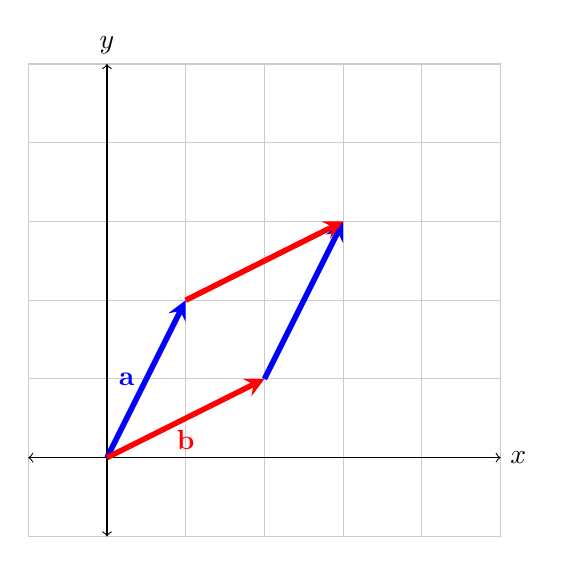
\begin{tikzpicture}
        \draw[thin,gray!40] (-1,-1) grid (5,5);
        \draw[<->] (-1,0)--(5,0) node[right]{$x$};
        \draw[<->] (0,-1)--(0,5) node[above]{$y$};
        \draw[line width=2pt,blue,-stealth](0,0)--(1,2) node[anchor=east] at (.5,1){$\mathbf{a}$};
        \draw[line width=2pt, red, -stealth](0,0)--(2,1) node[anchor=north] at (1,.5){$\mathbf{b}$};
        \draw[line width=2pt,blue,-stealth](2,1)--(3,3) node[anchor=east] at (.5,1){};
        \draw[line width=2pt, red, -stealth](1,2)--(3,3) node[anchor=north] at (1,.5){};
        \end{tikzpicture}
        \end{center}
        What is the area of this parallelogram? 
        \end{exercise}
        
        \begin{exercise}
        The area of the parallelogram defined by $\mathbf{a}=(3,1,-1)$ and $\mathbf{b}=(1,2,-3)$ can be found by computing $\|\mathbf{a}\times \mathbf{b}\|$.  Compute this.
        \end{exercise}
        
        \begin{ex}{Angular Velocity and Right-Hand Rule}{angular_velocity}
        For a particle moving along a circle with radius $r$ we can define a quantity called the \emph{angular velocity} and denote it by $\mathbf{\omega}$.  Then, for example, the time it takes for the particle to travel around the whole circle (the \emph{period}) is
        \[
        \tau = \frac{2\pi r}{\|\mathbf{\mathbf{\omega}}\|}.
        \]
        It turns out that the angular velocity of this particle at any point is given by
        \[
        \mathbf{\omega}=\frac{\mathbf{r}\times \mathbf{v}}{\|\mathbf{r}\|^2}.
        \]
        We can also find $\mathbf{v}$ from $\mathbf{\omega}$ and $\mathbf{r}$. Take a look at the figure below and note the orientation of $\mathbf{\omega}$ relative to the direction the particle travels around the circle.
        \begin{center}
        \begin{figure}[H]
            \centering
            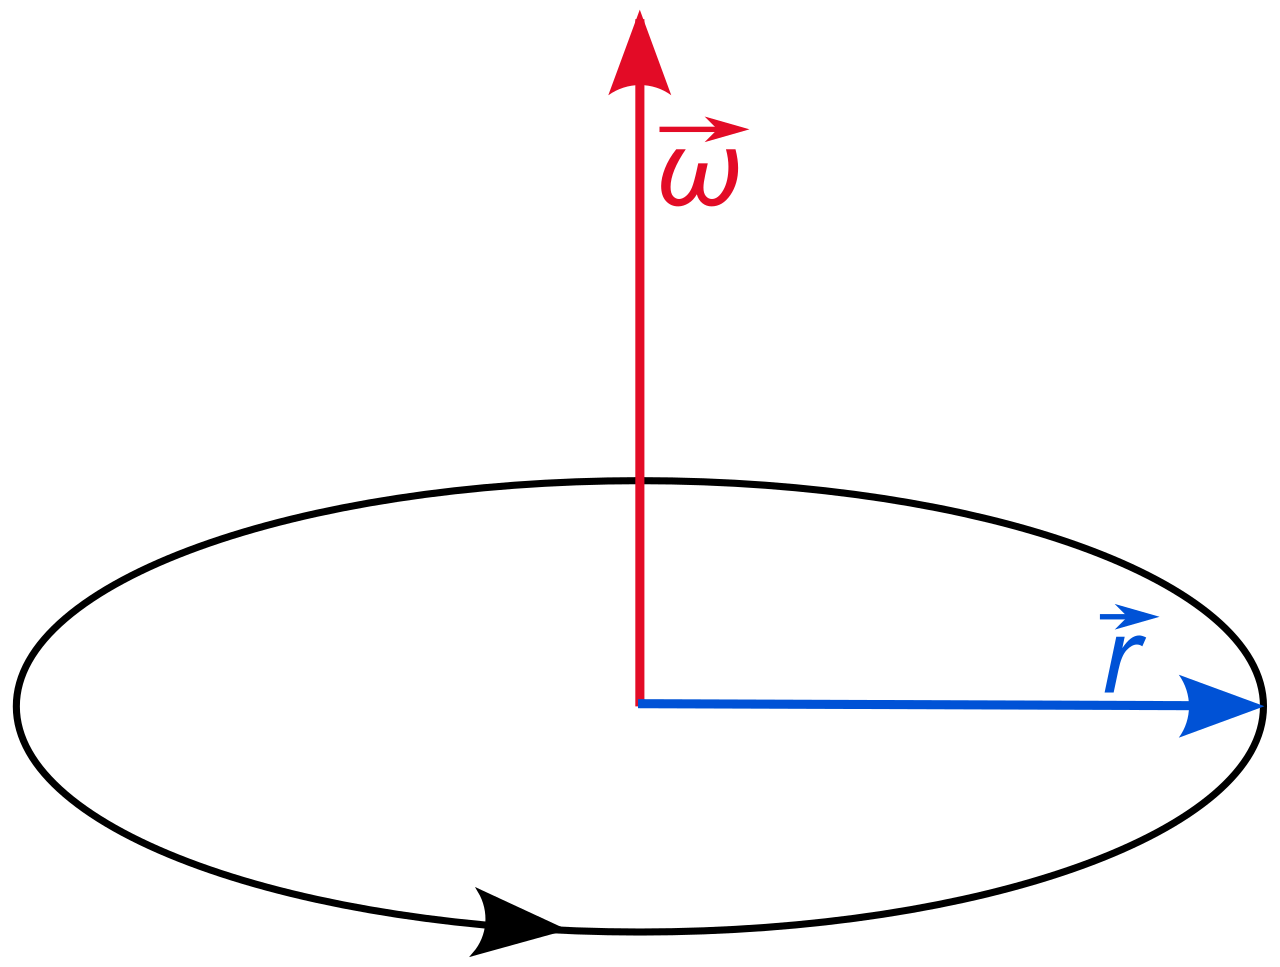
\includegraphics[width=.3\textwidth]{Figures/Angular_velocity.png}
            \caption{A particle moving around a circle of radius $\|\mathbf{r}\|$ in a counter-clockwise motion.}
            \label{angular-momentum}
        \end{figure}
        \end{center}
        Note that $\mathbf{v}$ would be tangent to this circle at the point $\mathbf{r}$ and pointing along the direction of travel.
        
        It turns out that $\mathbf{\omega}$ is a vector pointing perpendicularly to the plane that the circle the particle traverses is in. Which way does $\mathbf{\omega}$ point? We need the \emph{right-hand rule}!
        \begin{center}
        \begin{figure}[H]
            \centering
            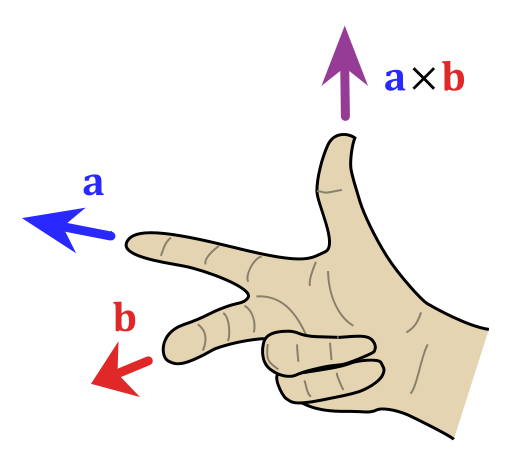
\includegraphics[width=.3\textwidth]{Figures/507px-Right_hand_rule_cross_product.png}
            \caption{The right-hand rule.}
        \end{figure}
        \end{center}
        To see how this works, we let $\mathbf{a}=\mathbf{r}$ be our index finger, then $\mathbf{v}=\mathbf{b}$ be our middle finger.  The resulting direction of $\mathbf{r}\times \mathbf{v}=\mathbf{\omega}$ is then pointing in the direction we see from Figure \ref{angular-momentum}.
        \end{ex}
        
        
    \chapter{Linear Transformations and Matrices}
        \section{Linear Transformations}
        Now that we have set the stage for vectors and the products between them, we would like to investigate how we can transform these vectors.  Specifically, we will first care about functions that are \emph{linear}.  These will be functions that stretch and rotate vectors and possibly change dimension all while leaving the origin alone.
        
        \begin{df}{Linear Transformation}{linear_transformation}
        A \textbf{linear transformation} \index{linear!transformation} is a function
        \[
        T\colon \R^n \to \R^m
        \]
        that satisfies the following requirements:
        \begin{enumerate}[(i)]
            \item $T(\mathbf{a}+\mathbf{b})=T(\mathbf{a})+T(\mathbf{b})$,
            \item $T(\lambda \mathbf{a})=\lambda T(\mathbf{a})$,
            \item $T(\mathbf{0})=\mathbf{0}$.
        \end{enumerate}
        \end{df}
        
        \begin{remark}
        These rules should seem similar to the properties of the derivative and integral.  We'll find that what we're building here will let us properly talk about derivatives in multiple dimensions.
        \end{remark}        
        
        \begin{ex}{Linear or Not?}{linear_or_not}
        Which of the following are linear transformations? Why or why not?
        \begin{enumerate}[(a)]
            \item $f\colon \R \to \R$ given by $f(x)=\lambda x$.
            \item $g\colon \R \to \R$ given by $g(x)=2x+1.$
            \item $h\colon \R \to \R$ given by $h(x)=x^2.$
            \item $T \colon \R^3 \to \R^3$ given by
            \[
            T\left( \begin{bmatrix} x\\ y\\ z \end{bmatrix} \right) = \begin{bmatrix} y\\ x\\ z \end{bmatrix}.
            \]
        \end{enumerate}
        \end{ex}
        
        \begin{ex}{Dot Product is Linear}{dot_prod_linear}
        If we choose a fixed vector $\mathbf{v}$, then the dot product of another vector $\mathbf{a}$ with $\mathbf{v}$ is itself an example of a linear transformation! It's also a good example of how the input dimension can differ from the output dimension.  Let us write $\textrm{Dot}_\mathbf{v}\colon \R^3 \to \R$ which is given by
        \[
        \textrm{Dot}_\mathbf{v}(\mathbf{a})=\mathbf{a}\cdot \mathbf{v}=a_xv_x+a_yv_y+a_zv_z.
        \]
        \end{ex}
        
        \begin{ex}{Scaling is Linear}
        Consider $T \colon \R^2 \to \R^2$ given by
        \[
        T\left( \begin{bmatrix} x\\ y \end{bmatrix}\right)
        = \begin{bmatrix} \lambda x\\ \gamma y \end{bmatrix}.
        \]
        This transformation scales the $x$-component of our vector by $\lambda$ and scales the $y$-component by $\gamma$.
        \end{ex}
        
        \begin{exercise}
        Pick a vector in the plane and draw a picture of the scaling transformation.
        \end{exercise}
        
        \begin{ex}{Rotation is Linear}
        Consider the following linear transformation $T\colon \R^2 \to \R^2$ given by
        \[
        T\left( \begin{bmatrix} x\\ y \end{bmatrix} \right)
        = \begin{bmatrix} x \cos \theta - y \sin \theta\\ x \sin \theta +y \cos \theta \end{bmatrix} = \begin{bmatrix} x'\\ y' \end{bmatrix}.
        \]
        This transformation rotates a vector by $\theta$ in the counter-clockwise direction. 
        \begin{figure}[H]
            \centering
            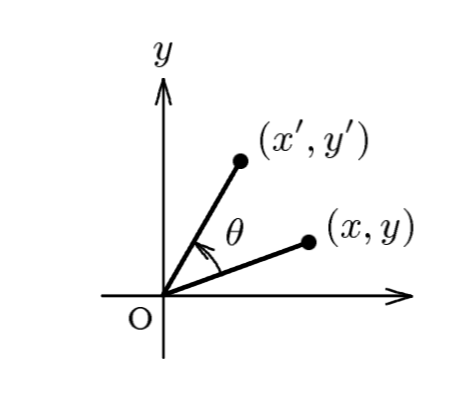
\includegraphics[width=.3\textwidth]{Figures/plane_rotation.png}
        \end{figure}
        \end{ex}
        
    \section{Matrices}
        
        The salient fact of linear transformations is how we can represent them.  As it turns out, any linear transformation $T\colon \R^n \to \R^m$ can be written like:
        \[
        T\left( \begin{bmatrix} x_1 \\ x_2 \\ \vdots \\ x_n \end{bmatrix}\right)
        = \begin{bmatrix} y_1 \\ y_2 \\ \vdots \\ y_m \end{bmatrix},
        \]
        where 
        \begin{align*}
            y_1 &= a_{11} x_1 + a_{12} x_2 + a_{13} x_3 + \cdots + a_{1n} x_n\\
            y_2 &= a_{21} x_1 + a_{22} x_2 + a_{23} x_3 + \cdots + a_{2n} x_n\\
            y_3 &= a_{31} x_1 + a_{32} x_2 + a_{33} x_3 + \cdots + a_{3n} x_n\\
            \vdots\\
            y_m &= a_{m1} x_1 + a_{m2} x_2 + a_{m3} x_3 + \cdots + a_{mn} x_n.
        \end{align*}
        The linear transformation is captured entirely by the \emph{matrix} of numbers
        \[
        \begin{bmatrix}
        a_{11} & a_{12} & a_{13} & \cdots & a_{1n}\\
        a_{21} & a_{22} & a_{23} & \cdots & a_{2n}\\
        a_{31} & a_{32} & a_{33} & \cdots & a_{3n}\\
        \vdots & \vdots & \vdots & & \vdots \\
        a_{n1} & a_{n2} & a_{n3} & \cdots & a_{nm}
        \end{bmatrix}
        \]
        
        We've seen that matrices are the fundamental object we need to describe linear transformations.  They aren't necessary to use, but they make computation and understanding a bit easier.  It turns out that we can also think of vectors as special cases of matrices, which makes the idea of studying matrices themselves all that much better. 
        
        \section{Matrix Algebra}
        Just as we did with vectors, we want to understand what we can do with these matrices algebraically.  
        
        We will call a matrix with $n$-rows and $m$-columns an \textbf{$n\times m$-matrix} (read: $n$ by $m$ matrix).  These take the form:
        \[\mathbf{A}=
        \begin{bmatrix}
        a_{11} & a_{12} & a_{13} & \cdots & a_{1n}\\
        a_{21} & a_{22} & a_{23} & \cdots & a_{2n}\\
        a_{31} & a_{32} & a_{33} & \cdots & a_{3n}\\
        \vdots & \vdots & \vdots & & \vdots \\
        a_{n1} & a_{n2} & a_{n3} & \cdots & a_{nm}
        \end{bmatrix}.
        \]
        We use a capital boldfaced letter to denote a matrix. Each entry of the matrix will be given by a lowercase letter with subscripts $a_{ij}$.  The subscripts will tell you which row and column the entry is located. For example, $a_{25}$ would be the entry in the 2$^\textrm{nd}$ row and $5^\textrm{th}$ column.
        
        \begin{enumerate}[(i)]
            \item \textbf{Equality:} Matrices are equal if each entry is equal. That is, given $\mathbf{A}$ and $\mathbf{B}$, we say $\mathbf{A}=\mathbf{B}$ if $a_{ij}=b_{ij}$ for each pair $i,j$.  Clearly if these matrices are not the same ``shape" (meaning, they have a different number of rows or columns), then they cannot be the same.  Just as a 2-dimensional vector cannot be the same as a 3-dimensional one.  They are distinctly different objects.
            
            \item \textbf{Addition:} We can add matrices of the same shape.  We write $\mathbf{A}+\mathbf{B}=\mathbf{C}$ and create the new matrix $\mathbf{C}$ by adding the entries.  That is, $c_{ij}=a_{ij}+b_{ij}$.  
            
            \item \textbf{Scalar Multiplication:} We can also scale matrices.  We do this by scaling the entries.  So, if we have $\lambda \mathbf{A}=\mathbf{B}$, then we know the entries of $\mathbf{B}$ are given by $b_{ij}=\lambda a_{ij}$.
            
            \item \textbf{Matrix Multiplication:} It is also possible to multiply two matrices together.  Recall that matrices are how we capture the information of a linear transformation. Matrix multiplication will capture the idea of composing two linear transformations. 
            
            We can multiply matrices $\mathbf{A}$ and $\mathbf{B}$ if 
            \[
            \textrm{the number of columns of $\mathbf{A}$}=\textrm{the number of rows of $\mathbf{B}$}.
            \]
            If $\mathbf{A}$ is an $n\times m$-matrix and $\mathbf{B}$ is an $m\times p$-matrix, then $\mathbf{C}=\mathbf{AB}$ is an $n\times p$ matrix.  You can remember this helpful fact:
            \[
            (n\times \underbrace{m)\cdot (m}_{\textrm{the same}}\times p)
            \]
            and
            \[
            (\underbrace{n}\times m)\cdot (m\times \underbrace{p})
            \]      
            gives the dimensions of the resulting matrix.
            
            How we perform this matrix multiplication looks a bit ugly at first, but it ends up being slightly easier after digesting this a bit. We have that the components of $\mathbf{C}=\mathbf{AB}$ are
            \[
            c_{ij}=\sum_{k=1}^m a_{ik}b_{kj}.
            \]
            
            Let us take the example of an $1\times n$-matrix $\mathbf{A}$ and a $n\times 1$-matrix $\mathbf{B}$. Then
            \[
            \mathbf{AB}=
            \begin{bmatrix} a_1 & a_2 & \cdots & a_n\end{bmatrix}
            \begin{bmatrix} b_1\\ b_2 \\ \vdots \\ b_n\end{bmatrix}=a_1b_1+b_2b_2+\cdots+a_nb_n=\sum_{k=1}^n a_kb_k.
            \]
            This is the dot product of two vectors!  As it turns out, we can decompose matrix multiplication into a bunch of dot products. 
            
            In general, the $i$th row of a matrix $\mathbf{A}$ is a vector with $m$ elements, the $j$th column of a matrix $\mathbf{B}$ is a vector with $m$ elements, and the dot product of these two vectors gives the entry $c_{ij}$ of the matrix $\mathbf{AB}=\mathbf{C}$.
            
            \begin{remark}
            This all means it is possible to take linear combinations of matrices as well!
            \end{remark}
            
            \begin{ex}{Multiplying Matrices}{multiplying_matrices}
            Let us multiply the following matrices:
            \[
            \mathbf{A}=\begin{bmatrix} 2 & 0 & -3\\ 1&1&-2\end{bmatrix} \quad \mathbf{B}=\begin{bmatrix} 2&3&4&1\\1&2&2&0\\0&-1&2&0\end{bmatrix}.
            \]
            Verify that you get
            \[
            \mathbf{AB}=\begin{bmatrix} 4&9&2&2\\3&7&2&1\end{bmatrix}.
            \]
            \end{ex}
            
            
            \subsubsection{Properties of Matrix Multiplication}
            
            Matrices will behave in the following ways:
            \begin{enumerate}[(i)]
                \item \textbf{Associativity:} The order in which you choose to multiply matrices does not matter.  That is 
                \[\mathbf{A}(\mathbf{BC})=(\mathbf{AB})\mathbf{C}=\mathbf{ABC}.\]
                \item \textbf{Distributivity:} We can multiply matrices over sums. That is
                \[
                \mathbf{A}(\mathbf{B}+\mathbf{C})=\mathbf{AB}+\mathbf{AC}.
                \]
                \item \textbf{(non)-Commutivity:} In general, we have
                \[
                \mathbf{AB}\neq \mathbf{BA}.
                \]
                However, there are certain types of matrices that do commute with each other.
            \end{enumerate}
            
            
        \end{enumerate}
        
        Right now we have the ability to write linear transformations as matrices.  We can also multiply these matrices.  Keep in mind that this in some way mimics composing functions.
        
    \section{The Determinant}
        We now want to understand further properties of matrices.  One important one is the \textbf{determinant.} The determinant is a special number associated to only $n\times n$-matrices.  We often call these matrices \emph{square}.  More on this later.  
        
        We can collect vectors $\mathbf{v}_1,\dots,\mathbf{v}_n$ into a matrix by placing each vector in a column of its own.  That is
        \[
        A=\begin{bmatrix}
        \mathbf{v}_1 &\mathbf{v}_2 &\cdots &\mathbf{v}_n
        \end{bmatrix}.
        \]
        If these are $n$-dimensional vectors, then this matrix is square.  Then the determinant of this matrix is written $\det(A)$. Let's now stick with just $2$ and $3$-dimensions as this will be all we need.
        
        \begin{example}[Area of a parallelogram]
        Say we have the vectors
        \[
        \mathbf{a}=\begin{bmatrix} 2\\ 0 \end{bmatrix} \quad \mathbf{b}=
        \begin{bmatrix} 1\\ 3 \end{bmatrix}.
        \]
        What is the area of the parallelogram that these vectors create? (See previous notes for how the cross product can do this.  We'll see that the cross product is highly related to determinants.)
        
        \begin{center}
        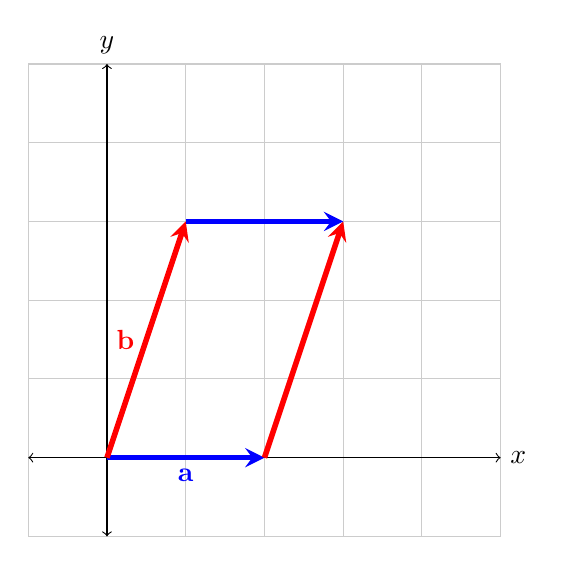
\begin{tikzpicture}
        \draw[thin,gray!40] (-1,-1) grid (5,5);
        \draw[<->] (-1,0)--(5,0) node[right]{$x$};
        \draw[<->] (0,-1)--(0,5) node[above]{$y$};
        \draw[line width=2pt,blue,-stealth](0,0)--(2,0) node[anchor=north] at (1,0){$\mathbf{a}$};
        \draw[line width=2pt, red, -stealth](0,0)--(1,3) node[anchor=east] at (.5,1.5){$\mathbf{b}$};
        \draw[line width=2pt,red,-stealth](2,0)--(3,3) node[anchor=east] at (.5,1){};
        \draw[line width=2pt, blue, -stealth](1,3)--(3,3) node[anchor=north] at (1,.5){};
        \end{tikzpicture}
        \end{center}
        The trick to finding the area here is to take move a triangle and fill in a gap. We do this like so:
        \begin{center}
        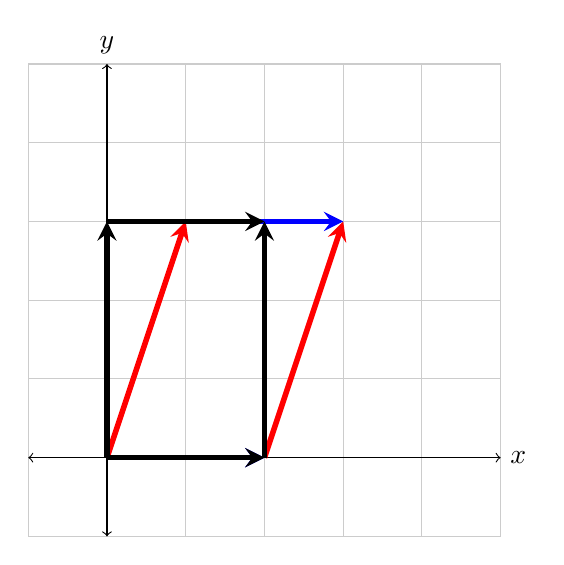
\begin{tikzpicture}
        \draw[thin,gray!40] (-1,-1) grid (5,5);
        \draw[<->] (-1,0)--(5,0) node[right]{$x$};
        \draw[<->] (0,-1)--(0,5) node[above]{$y$};
        \draw[line width=2pt,blue,-stealth](0,0)--(2,0) node[anchor=north] at (1,0){};
        \draw[line width=2pt, red, -stealth](0,0)--(1,3) node[anchor=east] at (.5,1.5){};
        \draw[line width=2pt,red,-stealth](2,0)--(3,3) node[anchor=east] at (.5,1){};
        \draw[line width=2pt, blue, -stealth](1,3)--(3,3) node[anchor=north] at (1,.5){};
        \draw[line width=2pt, black, -stealth](2,0)--(2,3) node[anchor=north] at (1,.5){};    
        \draw[line width=2pt, black, -stealth](0,0)--(0,3) node[anchor=north] at (1,.5){};
        \draw[line width=2pt, black, -stealth](0,0)--(2,0) node[anchor=north] at (1,.5){};
        \draw[line width=2pt, black, -stealth](0,3)--(2,3) node[anchor=north] at (1,.5){};
        \end{tikzpicture}
        \end{center}
        In the above, we've moved a triangle from the right, to the left, to make the black rectangle.  This rectangle then has an area of $2\cdot 3=6.$
        
        Let us see the way we can do this that does not require this extra work.  Let us place these vectors into a matrix:
        \[
        A=\begin{bmatrix} \mathbf{a} & \mathbf{b} \end{bmatrix}=
        \begin{bmatrix} 2 & 1\\ 0 & 3 \end{bmatrix}.
        \]
        Then $\det(A)$ will give us the area of this parallelogram! We have
        \[
        \det(A)=2\cdot 3 - 1\cdot 0 = 6.
        \]
        This begs the question, what is this formula in general?
        \end{example}
        
        To compute the determinant of a $2\times 2$-matrix
        \[
        A=\begin{bmatrix} a & b\\ c & d \end{bmatrix},
        \]
        we have
        \[
        \det(A) = ad-bc.
        \]
        You can remember this by thinking that you multiply top left with bottom right, then subtract the product of top right with bottom left.  
        \begin{ex}{Volume of a parallelopiped}{volume_of_parallelopiped}
        We often want to find volumes of parallelogram shaped higher dimensional objects.  In general, we call these \emph{parallelopipeds}.  
        
        For example, in $3$-dimensional space, we can take three vectors
        \[
        \mathbf{a}=\begin{bmatrix} 0 & 1 & 0 \end{bmatrix}\quad
        \mathbf{b}=\begin{bmatrix} 1 & 0 & 0 \end{bmatrix}\quad
        \mathbf{c}=\begin{bmatrix} 0 & 0 & 2 \end{bmatrix}.
        \]
        These, when combined properly, enclose a volume of a parallelopiped. 
\begin{center}
\tdplotsetmaincoords{60}{120} 
\begin{tikzpicture} [scale=3, tdplot_main_coords, axis/.style={->,black,thick}, 
vector/.style={-stealth,blue,very thick}, 
vector guide/.style={dashed,red,thick}]

%standard tikz coordinate definition using x, y, z coords
\coordinate (O) at (0,0,0);

%tikz-3dplot coordinate definition using x, y, z coords

\pgfmathsetmacro{\ax}{0.6}
\pgfmathsetmacro{\ay}{1}
\pgfmathsetmacro{\az}{0.8}

\coordinate (P) at (\ax,\ay,\az);

%draw axes
\draw[axis] (0,0,0) -- (1,0,0) node[anchor=north east]{$x$};
\draw[axis] (0,0,0) -- (0,1,0) node[anchor=north west]{$y$};
\draw[axis] (0,0,0) -- (0,0,1) node[anchor=south]{$z$};


\draw[line width=2pt, red, -stealth](0,0,0)--(0,3/4,0) node[anchor=north west] at (0,3/4,0){$\mathbf{a}$};
\draw[line width=2pt, blue, -stealth](0,0,0)--(1/4,0,0) node[anchor=north] at (1/4,0,0){$\mathbf{b}$};
\draw[line width=2pt, green, -stealth](0,0,0)--(0,0,1/2) node[anchor=east] at (0,0,1/2){$\mathbf{c}$};

\end{tikzpicture}
\end{center}
\begin{center}
\tdplotsetmaincoords{60}{120} 
\begin{tikzpicture} [scale=3, tdplot_main_coords, axis/.style={->,black,thick}, 
vector/.style={-stealth,blue,very thick}, 
vector guide/.style={dashed,red,thick}]

%standard tikz coordinate definition using x, y, z coords
\coordinate (O) at (0,0,0);

%tikz-3dplot coordinate definition using x, y, z coords

\pgfmathsetmacro{\ax}{0.6}
\pgfmathsetmacro{\ay}{1}
\pgfmathsetmacro{\az}{0.8}

\coordinate (P) at (\ax,\ay,\az);

%draw axes
\draw[axis] (0,0,0) -- (1,0,0) node[anchor=north east]{$x$};
\draw[axis] (0,0,0) -- (0,1,0) node[anchor=north west]{$y$};
\draw[axis] (0,0,0) -- (0,0,1) node[anchor=south]{$z$};


\draw[line width=2pt, red, -stealth](0,0,0)--(0,3/4,0) node[anchor=north west] at (0,1,0){};
\draw[line width=2pt, blue, -stealth](0,0,0)--(1/3,0,0) node[anchor=north] at (1/3,0,0){};
\draw[line width=2pt, green, -stealth](0,0,0)--(0,0,1/2) node[anchor=east] at (0,0,2/3){};

\draw[line width=2pt, red, -stealth](1/4,0,0)--(1/4,3/4,0) node[anchor=north west] at (1/3,2/3,3/3){};
\draw[line width=2pt, blue, -stealth](0,3/4,0)--(1/4,3/4,0) node[anchor=north] at (1/3,0,0){};
\draw[line width=2pt, green, -stealth](1/4,0,0)--(1/4,0,1/2) node[anchor=east] at (0,0,2/3){};

\draw[line width=2pt, red, -stealth](1/4,0,1/2)--(1/4,3/4,1/2) node[anchor=north west] at (1/3,2/3,3/3){};
\draw[line width=2pt, blue, -stealth](0,0,1/2)--(1/4,0,1/2) node[anchor=north] at (1/3,0,0){};
\draw[line width=2pt, green, -stealth](0,3/4,0)--(0,3/4,1/2) node[anchor=east] at (0,0,2/3){};

\draw[line width=2pt, red, -stealth](0,0,1/2)--(0,3/4,1/2) node[anchor=north west] at (1/3,2/3,3/3){};
\draw[line width=2pt, blue, -stealth](0,3/4,1/2)--(1/4,3/4,1/2) node[anchor=north] at (1/3,0,0){};
\draw[line width=2pt, green, -stealth](1/4,3/4,0)--(1/4,3/4,1/2) node[anchor=east] at (0,0,2/3){};
\end{tikzpicture}
\end{center}
Of course, I picked an easy example for the illustration.  But what is the volume? Here we again know we can compute this the usual way and we get that the volume is $1\cdot 1 \cdot 2 = 2.$

If we arrange these vectors in a matrix
\[
A=\begin{bmatrix} \mathbf{a} & \mathbf{b} &\mathbf{c} \end{bmatrix} =
\begin{bmatrix} 0 & 1 & 0 \\ 1 & 0 & 0 \\ 0 & 0 & 2 \end{bmatrix},
\]
we want $\det(A)$ to reflect this volume. It turns out the way we compute $\det(A)$ comes from using the determinant of $2\times 2$-matrices.  Let me explain further.

Let me write this matrix as a tool:
\[
\begin{bmatrix} + & - & +\\ - & + & - \\ + & - & + \end{bmatrix}.
\]
What we will use this for is a memory tool when we do something called the \emph{cofactor expansion}.  What I will do is choose a row of column to \emph{expand} across.  Let me choose the top row for simplicity's sake.  The top row will have signs $+-+$ that will show up in our computation. We will also have to take into account the element in the original matrix and multiply by that.

We start with the top left of $A$ and we will have a $+$ sign.  The top left of $A$ is element $a_{11}$ and so we remove the $1^{\textrm{st}}$ row and column from $A$ to give
\[
\textrm{Cof}_{11}(A)=\begin{bmatrix} 0 & 0 \\ 0 & 2 \end{bmatrix}.
\]
Then $\det(\textrm{Cof}_{11})(A))=0\cdot 2 - 0 \cdot 0=0.$

We now move on to the top middle of $A$ and will have a $-$ sign. The top middle element is $a_{12}$ and so we remove the $1^{\textrm{st}}$ row and $2^{\textrm{nd}}$ column of $A$ to give
\[
\textrm{Cof}_{12}(A)=\begin{bmatrix} 1 & 0 \\ 0 & 2\end{bmatrix}.
\]
Then $\det(\textrm{Cof}_{12}(A))=1\cdot 2-0 \cdot 0=2.$

Lastly, we move on to the top right of $A$ and will have a $+$ sign. The top right element is $a_{13}$ and so we remove the $1^{\textrm{st}}$ row and $3^{\textrm{rd}}$ column of $A$ to give
\[
\textrm{Cof}_{13}(A)=\begin{bmatrix} 1 & 0 \\ 0 & 0\end{bmatrix}.
\]
Then $\det(\textrm{Cof}_{12}(A))=1\cdot 0-0 \cdot 0=0.$

So $\det(A)=+(0)\cdot\det(\textrm{Cof}_{11}(A))-(1)\cdot\det(\textrm{Cof}_{12}(A))+(0)\cdot\det(\textrm{Cof}_{13}(A))=-2.$ So what we got was a negative of our predicted volume.
        \end{ex}

        \begin{exercise} Let
        \[
        A=\begin{bmatrix} 1 & 2 & 3 \\ 4 & 5 & 6 \\ 7 & 8 & 9 \end{bmatrix}.
        \]
        \begin{enumerate}[(a)]
            \item Find $\textrm{Cof}_{11}(A)$.
            \item Find $\textrm{Cof}_{22}(A)$.
            \item Find $\textrm{Cof}_{23}(A)$.
            \item Compute $\det(A)$.
        \end{enumerate}
        
        \end{exercise}
        
        \begin{question}
        What does it mean if $\det(A)=0$ for some matrix $A$?
        \end{question}
        
        \begin{answer}
        It means that we have a parallelopiped with zero volume.  Which means our three vectors actually lie in a plane, or even on a single line.  This is an important fact that will come up when we solve systems of equations!
        \end{answer}
        
        \begin{remark}
        Determinants can be computed in arbitrary dimension using the same process above.  It get's rather annoying and I do not find it necessary for us.
        \end{remark}
        
        \begin{remark}
        The sign of a determinant being negative has to do with an ``orientation" of the volume.  We like to choose ``right-handed" coordinates and its possible that the matrix, in a sense, can give us ``left-handed" coordinates.  This gives us a negative volume.
        \end{remark}
        
        \begin{ex}{Cross product from the Determinant}{cross_prod_det}
        You can compute the cross product from the determinant.  (You should be warned: this is an abuse of notation and a somewhat weird coincidence.) Let us create choose two vectors $\mathbf{v}$ and $\mathbf{w}$. We place them in a matrix $A$ as follows:
        \[
        A=
        \begin{bmatrix}
        \mathbf{\hat{\i}} & \mathbf{\hat{\j}} & \mathbf{\hat{k}}\\
        v_x & v_y & v_z\\
        w_x & w_y & w_z
        \end{bmatrix}.
        \]
        Then $\det(A)$ will give us the cross product $\mathbf{v}\times \mathbf{w}$.  Just know that you are briefly ignoring the fact that $\mathbf{\hat{\i}}$, $\mathbf{\hat{\j}}$, $\mathbf{\hat{k}}$ are actually vectors when you compute this.  Treat them as numbers until you get your final result.
        \end{ex}
        
        \begin{ex}{Determinant of a $3\times 3$-Matrix}{det_of_3x3}
        Let us write
        \[
        A=\begin{bmatrix} a_{11} & a_{12} & a_{13} \\ a_{21} & a_{22} & a_{23}\\ a_{31} & a_{32} & a_{33} \end{bmatrix}.
        \]
        We can expand across the first row and get
        \[
        \det(A)=a_{11}\cdot \det(\textrm{Cof}_{11}(A)) - a_{12}\cdot \det(\textrm{Cof}_{12}(A))+ a_{13}\cdot \det(\textrm{Cof}_{13}(A)).
        \]
        \end{ex}
        
        \begin{exercise}
        How could you write the determinant of a $3x3$-matrix $A$ that we expand along the second column?
        \end{exercise}
        
        \subsubsection{Properties of determinants}
        There are a few nice properties of determinants to keep in mind. 
        \begin{enumerate}[(i)]
            \item \textbf{Transposition:} If we exchange rows for columns in a matrix (that is, to take the \emph{transpose matrix}, then the value of the determinant is the same. Given
            \[
            A=\begin{bmatrix}
            a_{11} & a_{12} & a_{13}\\
            a_{21} & a_{22} & a_{23}\\
            a_{31} & a_{32} & a_{33}
            \end{bmatrix}
            \]
            we write the transpose matrix
            \[
            A^T=\begin{bmatrix}
            a_{11} & a_{21} & a_{31}\\
            a_{12} & a_{22} & a_{32}\\
            a_{13} & a_{23} & a_{33}
            \end{bmatrix}.
            \]
            So $a_{ij}\mapsto a_{ji}$. Then
            \[
            \det(A)=\det(A^T).
            \]
            
            \item \textbf{Multiplication by constants:} If we multiply a row or column by a scalar, then the determinant is also multiplied by that scalar.  So we have
            \[
            A_\lambda=\begin{bmatrix}
            \lambda a_{11} & \lambda a_{12} & \lambda a_{13}\\
            a_{21} & a_{22} & a_{23}\\
            a_{31} & a_{32} & a_{33}
            \end{bmatrix}
            \]
            Then
            \[
            \det(A_\lambda)=\lambda \det(A).
            \]
            
            \item \textbf{Addition of rows or columns:} If  we add to any row or column, then we can sum the determinants.  So we have
            \[
            \left| \begin{array}{ccc}
                a_{11} + v_1 & a_{12} & a_{13} \\
                a_{21} + v_2 & a_{22} & a_{23} \\
                a_{31} + v_3 & a_{32} & a_{33}
            \end{array}\right|=\left| \begin{array}{ccc}
                a_{11} & a_{12} & a_{13} \\
                a_{21} & a_{22} & a_{23} \\
                a_{31} & a_{32} & a_{33}
            \end{array}\right|+\left| \begin{array}{ccc}
                v_1 & a_{12} & a_{13} \\
                v_2 & a_{22} & a_{23} \\
                v_3 & a_{32} & a_{33}
            \end{array}\right|
            \]
            
            \item \textbf{Exchanging rows or columns:} If we swap rows or columns, the determinant is multiplied by $-1$. So we have
            \[
            \left|\begin{array}{ccc}
                a_{11} & a_{12} & a_{13} \\
                a_{21} & a_{22} & a_{23} \\
                a_{31} & a_{32} & a_{33}
            \end{array}\right|=-
            \left|\begin{array}{ccc}
                a_{12} & a_{11} & a_{13} \\
                a_{22} & a_{21} & a_{23} \\
                a_{32} & a_{31} & a_{33}
            \end{array}\right|
            \]
            
            \item \textbf{Linearly-dependent rows or columns:} If a column (resp. row) of a matrix can be written as a linear combination of the other two columns (resp. rows), then the determinant is zero.  This is basically saying that all three vectors lie in a single plane and so the volume of the parallelopiped given by the three vectors (as columns in the matrix) create no volume.
            
            Say we can write
            \begin{align*}
                a_{11}&=\lambda a_{12} + \mu a_{13}\\
                a_{21}&=\lambda a_{22} + \mu a_{23}\\
                a_{31}&=\lambda a_{32} + \mu a_{33}.
            \end{align*}
            Then $\det(A)=0.$
        \end{enumerate}
        
        These qualities of the determinant will give us the ability to analyze the next subsection properly.
        
        
        \section{Systems of Linear Equations}
        Often times we wish to solve equations of the form:
        \[
        A\mathbf{x}=\mathbf{b}
        \]
        where $A$ is an $n\times m$-matrix, $\mathbf{x}$ is an $m$-dimensional vector, and $\mathbf{b}$ is an $n$-dimensional vector.  Let us write out what this looks like:
        \[
        \begin{bmatrix}
        a_{11} & a_{12} & \cdots & a_{1m}\\
        a_{21} & a_{22} & \cdots & a_{2m}\\
        \vdots & \vdots & \cdots & \vdots\\
        a_{n1} & a_{n2} & \cdots & a_{nm}
        \end{bmatrix}
        \begin{bmatrix}
        x_1\\ x_2 \\ \vdots \\ x_m
        \end{bmatrix}
        =\begin{bmatrix}
        b_1 \\ b_2 \\ \vdots \\ b_n
        \end{bmatrix},
        \]
        gives us a set of equations
        \begin{align*}
        a_{11} x_1 + a_{12}x_2 + \cdots a_{1m} x_m &= b_1\\
        a_{21} x_1 + a_{22} x_2 + \cdots a_{2m} x_m &= b_2
        &\vdots\\
        a_{n1} x_1 + a_{n2} x_2 + \cdots a_{nm} x_m &= b_n.
        \end{align*}
        We call these equations a \textbf{system of linear equations}.
        
        In general, if $n\neq m$, the methods of solving are exactly what we will cover aside from the ability to use the determinant.  However, there are some subtle issues with the $n\neq m$ case that I won't go into detail on.  If you're interested, look up \emph{over} and \emph{underdetermined} systems. From this point on we will assume $A$ to be $n\times n$.
        
        \subsubsection{Homogeneous Equations}
        Let us begin with the easiest case to analyze, the \textbf{homogeneous equations}. These take the form 
        \[
        A\mathbf{x}=\mathbf{0}.
        \]
        This yields the equations:
        \begin{align*}
            a_{11}x_1 + a_{12}x_2 + \cdots + a_{1n}x_n &=0\\
            a_{21}x_1 + a_{22} x_2 + \cdots + a_{2n}x_n &=0\\
            &\vdots\\
            a_{n1}x_1 +a_{n2}+ \cdots +a_{nn}x_n &=0.
        \end{align*}
        
        \begin{prop}{Solutions to Homogeneous Equations}{solutions_to_homo}
        The homogeneous equations have solutions:
        \begin{itemize}
            \item (Trivial) $\mathbf{x}=\mathbf{0}$ if and only if $\det(A)\neq 0$;
            \item $\mathbf{x}\neq \mathbf{0}$ if and only if $\det(A)= 0$.
        \end{itemize}
        \end{prop}
        
        \begin{exercise}
        Take the determinant and then attempt to solve the following homogeneous equations.
        \begin{enumerate}[(a)]
            \item Let 
            \[
            A=\begin{bmatrix}
            1 & 1 & 0\\
            1 & 0 & 5\\
            0 & 1 & 2
            \end{bmatrix}
            \]
            and solve $A\mathbf{x}=\mathbf{0}.$
            \item Let
            \[
            B=\begin{bmatrix}
            2 & 3 & 1\\
            1 & 4 & 3\\
            1 & 2 & 1
            \end{bmatrix}
            \]
            and solve $B\mathbf{x}=\mathbf{0}.$
        \end{enumerate}
        \end{exercise}
        
        \begin{remark}
        Notice that in (b), if we add column one to column three for the matrix $B$, that we end up with column two.  This means if we treat the columns of $B$ as vectors; that is, we let
        \[
        \mathbf{v}_1=\begin{bmatrix}
        2 \\ 1 \\ 1
        \end{bmatrix} \quad 
        \mathbf{v}_2= \begin{bmatrix} 3 \\ 4 \\ 2 \end{bmatrix} \quad
        \mathbf{v}_3= \begin{bmatrix} 1 \\ 3 \\ 1 \end{bmatrix}.
        \]
        Then $\mathbf{v}_2=\mathbf{v}_1+\mathbf{v}_3$.  This means all these vectors lie in a plane, and the determinant of $B$ should be zero based on our intuition.  It also means we can solve
        \[
        \lambda_1 \mathbf{v}_1 + \lambda_2 \mathbf{v}_2 + \lambda_3 \mathbf{v}_3 = \mathbf{0}
        \]
        where $\lambda_1$, $\lambda_2$, and $\lambda_3$ are not all zero.
        
        This is a very important realization in the realm of linear systems.  With our limited time and scope, we cannot possibly do everything here.  But, keep this in mind.  There is a strong relationship between the geometry of the set of solutions and the algebra of vectors and matrices.  If this seems interesting to you, consider taking Math 369.
        \end{remark}
        
        \section{Solving Linear Systems of Equations}
        Say we are handed a matrix $A$ and an output vector $\mathbf{b}$ and we are asked to solve
        \[
        A\mathbf{x}=\mathbf{b}
        \]
        for the vector $\mathbf{x}$. If $\mathbf{b}$ is nonzero, then we call this an \textbf{inhomogeneous} linear system. If $A$ is a square matrix, we can say more.
        
        \begin{prop}{Solutions to Inhomogeneous Equations}{solutions_to_inhomo}
        The inhomogenous equations have solutions:
        \begin{itemize}
            \item A unique solution if and only if $\det(A)\neq 0$;
            \item None or possibly infinitely many solutions if $\det(A)=0$.
        \end{itemize}
        \end{prop}
        
        This proposition should feel remniscent of the case for functions $f\colon \R\to \R$.  In this case, we may have been handed a function $f$, a $y$ (output) value, and were asked to find what input $x$ corresponds to that $y$ value. That is, we want
        \[
        f(x)=y.
        \]
        Here we could sometimes find an inverse function $f^{-1}$ that would satisfy
        \[
        f^{-1}(y)=x.
        \]
        However, for example, if we had the function $f(x)=x^2$, then there was no inverse function.  Why? Well, say we let $y=1$, then $x=\pm 1$ are both solutions. More on inverses later.  
        
        For now we need a method to solve the equation $A\mathbf{x}=\mathbf{b}$ for $\mathbf{x}$. 
        
        \begin{df}{Row Operations}{row_operations}
        We call the following list of operations the \textbf{elementary row operations}.
        \begin{itemize}
            \item \textbf{Row scaling:} We can scale the rows of a matrix by any scalar value $\lambda$.
            \item \textbf{Row addition:} We can add scalar multiples of any rows to another row.
            \item \textbf{Row swapping:} We can swap any two rows.
        \end{itemize}
        These operations are elementary in the sense that they do not change the ``character" of the determinant.  This means that these will not affect the solution to our system as it will not spontaneously make a determinant change from nonzero to zero or vice-versa.  
        \end{df}
        
        \begin{df}{Augmented Matrix}{augmented_matrix}
        Given an equation $A\mathbf{x}=\mathbf{b}$, we have the \textbf{augmented matrix} \index{augmented matrix} $M$
        \[
        M=\left[\begin{array}{ccc|c}
        a_{11} & a_{12} & a_{13}  &  b_1 \\
        a_{21} & a_{22} & a_{23} & b_2\\
        a_{31} & a_{32} & a_{33} & b_3
        \end{array}\right]
        \]
        (Of course, this is just for the $3\times 3$-case.  It looks similar for the $n\times n$-case.)
        \end{df}
        
        Our goal here is to use elementary row operations to reduce our augmented matrix to the following \textbf{row echelon form}.  This will look like:
        \[
        M=\left[\begin{array}{ccc|c}
        m_{11} & m_{12} & m_{13}  &  c_1 \\
        0 & m_{22} & a_{23} & c_2\\
        0 & 0 & m_{33} & c_3
        \end{array}\right]
        \]
        where the $m_{ij}$ and $c_k$ are all (possibly) new entries since we have performed elementary row operations.  It can also be that, for example, $m_{33}$ is also zero. This will be important. This is all a bit nebulous. Let us do an example. 
        
        \begin{ex}{A System of Inhomogeneous Equations}{system_of_inhomo}
        Let us consider the following matrix equation:
        \[
        \begin{bmatrix}
        1 & 0 & 2\\
        2 & 2 & 3\\
        4 & 4 & 1
        \end{bmatrix}
        \begin{bmatrix}
        x\\
        y\\
        z
        \end{bmatrix}
        =\begin{bmatrix}
        1\\
        1\\
        1
        \end{bmatrix}.
        \]
        This gives us the following system of linear equations:
        \begin{align*}
            1x+0y+2z&=1\\
            2x+2y+3z&=1\\
            4x+4y+1z&=1.
        \end{align*}
        You can solve this by hand, but it is tedious.  We will use the row reduction technique instead.  Let us create the augmented matrix
        \[
        \left[\begin{array}{ccc|c}
        1 & 0 & 2 & 1 \\
        2 & 2 & 3 & 1 \\
        4 & 4 & 1 & 1
        \end{array}\right].
        \]
        We can then do row operations to get our result
        \[
        \left[\begin{array}{ccc|c}
        1 & 0 & 2 & 1 \\
        2 & 2 & 3 & 1 \\
        4 & 4 & 1 & 1
        \end{array}\right] \underrightarrow{-2 R_2 \textrm{ from } R_3} 
        \left[\begin{array}{ccc|c}
        1 & 0 & 2 & 1 \\
        2 & 2 & 3 & 1 \\
        0 & 0 & -5 & -1
        \end{array}\right]
        \]
        then
        \[
        \left[\begin{array}{ccc|c}
        1 & 0 & 2 & 1 \\
        2 & 2 & 3 & 1 \\
        0 & 0 & -5 & -1
        \end{array}\right] \underrightarrow{-2 R_1 \textrm{ from } R_2} 
        \left[\begin{array}{ccc|c}
        1 & 0 & 2 & 1 \\
        0 & 2 & -1 & -1 \\
        0 & 0 & -5 & -1
        \end{array}\right]   .     
        \]
        Notice now we have the equations
        \begin{align*}
            1x+0y+2z&=1\\
            0x+2y-1z&=-1\\
            0x+0y-5z&=-1.
        \end{align*}
        These we can now easily solve.  Specifically we get
        \[
        z=\frac{1}{5} ~\implies~ y=\frac{-2}{5} ~\implies~ x=\frac{3}{5}. 
        \]
        Double check my work above.  But we can also plug in our vector now to verify our result.  That is
        \[
        \begin{bmatrix}
        1 & 0 & 2\\
        2 & 2 & 3\\
        4 & 4 & 1
        \end{bmatrix}
        \begin{bmatrix}
        3/5\\
        -2/5\\
        1/5
        \end{bmatrix}
        =\begin{bmatrix}
        1\\
        1\\
        1
        \end{bmatrix}.        
        \]
        \end{ex}
        
        \begin{ex}{System of Homogeneous Equations}{system_of_homo}
        Let us take the matrix we had previously,
        \[
        B=\begin{bmatrix}
        2 & 3 & 1\\
        1 & 4 & 3\\
        1 & 2 & 1
        \end{bmatrix}
        \]
        and solve for the vector $\mathbf{x}$ so that $B\mathbf{x}=\mathbf{0}$. Then the augmented matrix
        \[
        M=\left[\begin{array}{ccc|c}
        2 & 3 & 1  &  0 \\
        1 & 4 & 3 & 0\\
        1 & 2 & 1 & 0
        \end{array}\right].
        \]
        Now we can perform row operations.  It will be good to keep track of what you do as I do.
        \[
        \left[\begin{array}{ccc|c}
        2 & 3 & 1  &  0 \\
        1 & 4 & 3 & 0\\
        1 & 2 & 1 & 0
        \end{array}\right] \underrightarrow{-1/2 R_1 \textrm{ from } R_2 \textrm{ and } R_3} 
        \left[\begin{array}{ccc|c}
        2 & 3 & 1  &  0 \\
        0 & 5/2 & 5/2 & 0\\
        0 & 1/2 & 1/2 & 0
        \end{array}\right]
        \]
        \[
        \left[\begin{array}{ccc|c}
        2 & 3 & 1  &  0 \\
        0 & 5/2 & 5/2 & 0\\
        1 & 1/2 & 1/2 & 0
        \end{array}\right] \underrightarrow{-1/5 R_2 \textrm{ from } R_3} 
        \left[\begin{array}{ccc|c}
        2 & 3 & 1  &  0 \\
        0 & 5/2 & 5/2 & 0\\
        0 & 0 & 0 & 0
        \end{array}\right]
        \]
        Notice that the whole last row is all $0$ now.  This corresponds to the equation:
        \[
        0x+0y+0z=0.
        \]
        We call $z$ a \textbf{free variable} since we could choose any value for it.  \emph{It is important that we only let $z$ here be free.  The other variables are still to be decided since they appear in the rows above.}  I'll let $z=t.$  
        
        The middle row corresponds to the equation:
        \[
        0x+\frac{5}{2}y+\frac{5}{2}z=0.
        \]
        Recall I let $z=t$ and we can now solve for $y$, but not $x$ (yet) as it appears in the row above.  This gives us that $y=-t$.
        
        The top row corresponds to the equation:
        \[
        2x+3y+1z=0.
        \]
        We now just determine $x$ by using the values of $y$ and $z$ we just found. So,
        \begin{align*}
        2x+3(-t)+1(t)&=0\\
        2x=2t\\
        x=t.
        \end{align*}
        So I claim that the solution here is the vector
        \[
        \mathbf{x}=\begin{bmatrix} t \\ -t \\ t\end{bmatrix},
        \]
        where $t$ is \emph{any} real number.  Let's check this:
        \[
        \begin{bmatrix}
        2 & 3 & 1\\
        1 & 4 & 3\\
        1 & 2 & 1
        \end{bmatrix}
        \begin{bmatrix}
        t\\
        -t\\
        t
        \end{bmatrix}
        =\begin{bmatrix}
        0\\
        0\\
        0
        \end{bmatrix}.
        \]
        So we are happy.  We found a solution! In fact, we found infinitely many solutions.  It turns out that anything on this \emph{line} is a solution.
        
        \end{ex}
        

        
    \section{The Inverse Matrix}
        Often times when we are solving the equation
        \[
        A\mathbf{x}=\mathbf{b}
        \]
        for $\mathbf{x}$, we can actually do this is in more generality.
        
        What I mean is that we may be able to find a matrix $A^{-1}$ so that we can do 
        \begin{align*}
            A^{-1}A\mathbf{x}&=A^{-1}\mathbf{b}\\
            \mathbf{x}&=A^{-1}\mathbf{b}.
        \end{align*}
        We call this special matrix $A^{-1}$ the \textbf{inverse matrix}. In this case $A$ must be square or else this is not at all possible! If $A$ has an inverse matrix we say that $A$ is \textbf{invertible}.
        
        Since $A$ is a function (specifically, a linear transformation), we do not always have an inverse. However, we have a tool at our disposal that tells us whether we have an inverse or not. 
        
        Let us create a necessary definition first.
        
        \begin{df}{Identity Matrix}{identity_matrix}
        We call the matrix $I$ with entries 
        \[I_{ij}=
        \begin{cases}
        1 \textrm{ if } i=j\\
        0 \textrm{ elsewise}
        \end{cases}
        \]
        the \textbf{identity matrix}\index{identity matrix}.  For example, the $3\times 3$ identity matrix is
        \[
        \begin{bmatrix}
        1 & 0 & 0\\
        0 & 1 & 0\\
        0 & 0 & 1
        \end{bmatrix}.
        \]
        \end{df}
        
        Why do we call this the identity matrix? Well, it's because we have the following:
        
        \begin{prop}{Identity Matrix Fixes Vectors}{identity_fixes_vectors}
        For any vector $\mathbf{v}$ we have that
        \[
        I\mathbf{v}=\mathbf{v}.
        \]
        In fact, for any square matrix $A$, we have that
        \[
        IA=AI=A.
        \]
        \end{prop}
        
        \begin{exercise}
        Let
        \[
        \mathbf{v}=\begin{bmatrix} 1 \\ 2 \\ 3 \end{bmatrix}.
        \]
        Show that
        \[
        I\mathbf{v}=\mathbf{v}.
        \]
        
        Similarly, let
        \[
        A= \begin{bmatrix}
        1 & 2 & 3\\
        4 & 5 & 6\\
        7 & 8 & 9
        \end{bmatrix}.
        \]
        Show that
        \[
        IA=A.
        \]
        \end{exercise}
        
        Now that we have this defined, we can get back to inverses.
        
        \begin{prop}{Existence of Inverse}{existence_of_inverse}
        If $\det(A)\neq 0$, then $A^{-1}$ exists and is unique.
        \end{prop}
        
        Then, if one exists, how would we compute it?  In short, we already know how.
        
        \subsubsection{Inverting a matrix}
        
        Let $A$ be an invertible matrix.  Then we construct $A^{-1}$ as follows.  We create an augmented matrix
        \[
        M=
        \left[ \begin{array}{ccc|ccc}
        a_{11} & a_{12} & a_{13} & 1 & 0 & 0 \\
        a_{21} & a_{22} & a_{23} & 0 & 1 & 0 \\
        a_{31} & a_{32} & a_{33} & 0 & 0 & 1 
        \end{array} \right].
        \]
        Then we row reduce the left portion until we have
        \[
        \left[ \begin{array}{ccc|ccc}
        1 & 0 & 0 & a_{11}^{-1} & a_{12}^{-1} & a_{13}^{-1}\\
        0 & 1 & 0 & a_{21}^{-1} & a_{22}^{-1} & a_{23}^{-1} \\
        0 & 0 & 1 & a_{31}^{-1} & a_{32}^{-1} & a_{33}^{-1} 
        \end{array} \right],
        \]
        where $a_{ij}^{-1}$ is the entry of the matrix $A^{-1}$.  \emph{It's important to note that I do not mean that $a_{ij}^{-1}=1/a_{ij}$!}
        
        \begin{exercise}
        Let
        \[
        A=\begin{bmatrix}
        1 & 2\\
        2 & 1
        \end{bmatrix}.
        \]
        \begin{enumerate}[(a)]
            \item Find $A^{-1}$.
            \item Compute $\det(A)$ and $\det(A^{-1})$. What do you notice about $\det(A^{-1})$ compared to $\det(A)$?
        \end{enumerate}
        \end{exercise}
        
        \begin{prop}{Determinant of Inverse Matrix}{det_of_inverse}
        We have that for matrices $A,B$ that $\det(AB)=\det(A)\det(B)$.  It follows that 
        $\det(AA^{-1})=1$ and so 
        \[
        \det(A^{-1})=\frac{1}{\det(A)}.
        \]
        \end{prop}
    
        
   \section{The Eigen-Problem}
   \index{eigen}
        A question of fundamental importance is as follows. 
        \begin{question}
        Given a square matrix $A$, are there scalars $\lambda$ and vectors $\mathbf{v}$ where
        \[
        A\mathbf{v}=\lambda \mathbf{v}?
        \]
        \end{question}
        
        \begin{answer}
        In short, the answer is yes.  However, this question has some subtleties to it that we will avoid in order to understand the main concept.
        \end{answer}
        
        \begin{df}{Eigenvalues and Eigenvectors}{eigenvals_eigenvects}
        Let $A$ be a square matrix.  Then if we have a scalar $\lambda$ and $\mathbf{v}$ satisfying
        \[
        A\mathbf{v}=\lambda \mathbf{v}
        \]
        we call $\lambda$ an \textbf{eigenvalue} \index{eigen!value} and $\mathbf{v}$ the corresponding \textbf{eigenvector}\index{eigen!vector}.
        \end{df}
        
        \begin{remark}
        \begin{itemize}
            \item Eigen is a German word that translates to ``own" in English.
            \item It's important to note that an eigenvalue \emph{corresponds} to an eigenvector.  They are insperable friends! 
        \end{itemize}
        \end{remark}
        
        \begin{question}
        Why in the world should we care about this? What are the applications? 
        \end{question}
        
        \begin{answer}
        \begin{itemize}
            \item First off, mathematically what this is saying is we can find vectors that are affected by a linear transformation (a matrix $A$) in the simplest possible way.  That is, the matrix just scales the vector!  If we are able to find a \emph{basis} of eigenvectors, then we can understand how a matrix $A$ acts entirely by scaling certain \emph{directions}. This last part is not always possible, but we are not concerned with this.
            \item The applications are extremely far ranging.  
            \begin{itemize}
                \item Data analysis: Understanding the structure of a data set.
                \item Mechanics: Understanding rotational motion.
                \item Quantum Mechanics: The whole theory of ``first quantization" is solving an eigen-equation usually referred to as \emph{Sch\"odinger's equation}. Spin systems (i.e., electrons and photons) are the direct analog to what we do here.
                \item Molecular Orbitals: Molecular orbitals are eigenvectors of the Fock operator.
                \item Differential Equations: We can often recast differential equations as eigen-problems which are, in general, fairly easy to solve in comparison. Here eigenvectors are functions.
                \item Finance: Breaking down portfolios based on risk and returns.
                \item Geology: The study of glacial till.
                \item Principal Component Analysis: A generalization of the eigen-problem.
            \end{itemize}
            There are certainly more that I'm unaware of.  Maybe this is a good project idea for you!
        \end{itemize}
        \end{answer}
        
        Great, so now we are motivated.  But, how can we hope to find these eigenvalues and eigenvectors?  
        
        We begin with the equation
        \[
        A\mathbf{v}=\lambda \mathbf{v}
        \]
        and we move everything to the left side to yield
        \begin{align*}
            A\mathbf{v}-\lambda \mathbf{v}&=0.
        \end{align*}
        Remember that we can multiply by the identity matrix and not change a single thing.  We do this like so.
        \begin{align*}
            A\mathbf{v}- I \lambda \mathbf{v}&=0\\
            (A-\lambda I)\mathbf{v}&=0.
        \end{align*}
        This means we have reduced the problem to solving the homogeneous equations for a slightly different matrix $A-\lambda I$.  
        
        Recall that we had a proposition that said these homogeneous equations have nontrivial solutions if 
        \[
        \det(A-\lambda I)=0.
        \]
        (\emph{Careful. The difference between homogeneous and inhomogeneous equations makes the condition on the determinant different!)}
        
        This determinant condition gives us an equation for $\lambda$. When we then know $\lambda$, we can solve for $\mathbf{v}$ by plugging in the known $\lambda$ value and solving the homogeneous equations. Let me put this down in an algorithmic way.
        
        \begin{enumerate}
            \item Let $\lambda$ be a variable.  Then we make the matrix $A-\lambda I$.
            \item Take the determinant of $A-\lambda I$ and set it equal to zero. That is,
            \[
            \det(A-\lambda I)=0.
            \]
            This will give you a polynomial equation with the variable $\lambda$.  Worst case for us is having to solve the quadratic equation.  
            \item You will find (possibly) multiple values of $\lambda$ from the determinant above.  
            \item For each $\lambda_i$, you will find an eigenvector $\mathbf{v}_i$ by solving the homogeneous equation
            \[
            (A-\lambda_i I)\mathbf{v}_i=0.
            \]
            These will always give you a free variable if done correctly.  
        \end{enumerate}
        
        \begin{ex}{Eigenvalues of a Diagonal Matrix}{eigenvalues_of_diagonal}
        The easiest example of the eigenvalue problem is finding the eigenvectors and eigenvalues of a \emph{diagonal} matrix.  In this case, let
        \[
        A=\begin{bmatrix}
        1 & 0 & 0\\
        0 & 2 & 0\\
        0 & 0 & 3
        \end{bmatrix}.
        \]
        \begin{enumerate}
            \item Take $\lambda$ to be a variable and put
            \[
            A-\lambda I = \begin{bmatrix}
            1-\lambda & 0 & 0\\
            0 & 2-\lambda & 0\\
            0 & 0 & 3-\lambda
            \end{bmatrix}.
            \]
        \item Now we take the determinant of $A-\lambda I$
        \[
        \det(A-\lambda I)= (1-\lambda)(2-\lambda)(3-\lambda).
        \]
        We set this equal to zero
        \[
        (1-\lambda)(2-\lambda)(3-\lambda)=0.
        \]
        \item Note that this has solutions $\lambda_1=1$, $\lambda_2=2$, and $\lambda_3=3$.  Make sure you're comfortable with this.
        \item 
        \begin{itemize}
            \item \textbf{$\lambda_1=1$:} We take
            \[
            (A-1I)\mathbf{v}=0.
            \]
            We solve this by making the augmented matrix:
            \[
            M=\left[ \begin{array}{ccc|c}
                 1-1 & 0 & 0 & 0\\
                 0 & 2-1 & 0 & 0\\
                 0 & 0 & 3-1 & 0
            \end{array}\right].
            \]
            We can then perform the row reduction steps to get this augmented matrix to RREF.  In our case, this is essentially done and the system of equations reads:
            \begin{align*}
                0x+0y+0z&=0 ~\implies~ x=t\\
                0x+1y+0z&=0 ~\implies~ y=0\\
                0x+0y+2z&=0 ~\implies~ z=0.
            \end{align*}
            So we have a solution
            \[
            \mathbf{v}_1 =\begin{bmatrix}
            t\\ 0\\ 0\\
            \end{bmatrix}.
            \]
            We usually take $t=1$ and say that the eigenvector is 
            \[
            \mathbf{v}_1 =\begin{bmatrix}
            1\\ 0 \\ 0
            \end{bmatrix}.
            \]
            \item \textbf{$\lambda_2=2$:} I'll suppress the work here but the eigenvector is
            \[
            \mathbf{v}_2 = \begin{bmatrix}
            0 \\ 1 \\ 0
            \end{bmatrix}.
            \]
            \item \textbf{$\lambda_3=3$:} Again, the eigenvector is
            \[
            \mathbf{v}_3=\begin{bmatrix}
            0 \\ 0 \\ 1
            \end{bmatrix}.
            \]
        \end{itemize}
        \end{enumerate}
        \end{ex}

\begin{center}
\Large{Worksheet: Eigensystems}
\end{center}


\normalsize

\begin{problem} Consider the matrix 
\[
A= \begin{bmatrix}
3 & 0\\
0 & -3
\end{bmatrix}.
\]
\begin{enumerate}[(a)]
    \item Compute $\det(A-\lambda I)$.
    \item Find the solutions $\lambda$ for $\det(A-\lambda I)=0$.  These are your eigenvalues.
    \item Solve 
    \[
    (A-\lambda_1)\mathbf{v}_1=\mathbf{0}
    \]
    where $\lambda_1$ is your first eigenvalue. This will give you the corresponding eigenvector $\mathbf{v}_1$.
    \item Solve 
    \[
    (A-\lambda_2)\mathbf{v}_2=\mathbf{0}
    \]
    where $\lambda_2$ is your first eigenvalue. This will give you the corresponding eigenvector $\mathbf{v}_2$.
    \item Do you notice anything about the eigenvalues and the matrix $A$? What about the $\det(A)$ and the eigenvalues?
\end{enumerate}
\end{problem}

\begin{problem}
Consider the matrix
\[
A=\begin{bmatrix}
0 & 5\\
5 & 0
\end{bmatrix}.
\]
Repeat the process given in Problem 1 to determine the two eigenvalues and eigenvectors for $A$.
\end{problem}

\begin{problem}
Consider the matrix 
\[
A=
\begin{bmatrix}
0 & -1\\
1 & 0
\end{bmatrix}.
\]
What happens when we try to find
\[
\det(A-\lambda I)=0? 
\]
How must we resolve this issue?
\end{problem}

        


\part{Vector Calculus}

    \chapter{The Complex Numbers}
        
        \section{Introduction to Complex Numbers}
        
        Complex numbers are the next topic for us to investigate.  They are a useful tool throughout mathematics and the sciences. 
        
        Part II is about ``Multivariable Calculus" and complex functions provide us a good foray into this realm.  Though we will not investigate the differential calculus structure on the complex numbers $\C$, we will gain intuition for the future.  As a topic in itself, complex numbers are fascinating.
        
        \begin{question}
        What is a complex number? What is the motivation for developing them?
        \end{question}
        
        \begin{answer}
        Let me begin by answering the second part of the question.  
        
        Take a polynomial,
        \[
        a_0+a_1 z + a_2 z^2 + \cdots + a_n z^n.
        \]
        When does this polynomial equal zero?  In other words, what are the \emph{roots} of this polynomial?
        
        The fact of the matter is that the real numbers $\R$ are just not large enough to guarantee that we have all possible roots. Take, for example, the polynomial
        \[
        x^2+1.
        \]
        Set this equal to zero and we have
        \begin{align*}
            x^2+1&=0\\
            \implies x^2&=-1\\
            \implies x&=\pm \sqrt{-1}.
        \end{align*}
        It seems that we are missing a number in this case.  Specifically, 
        \[
        \sqrt{-1}\notin \R.
        \]
        Let us take this new number and denote
        \[
        i=\sqrt{-1}.
        \]
        Of course this also means that
        \[
        i^2=-1.
        \]
        
        A complex number will be made with real numbers and this new additional member. 
        \end{answer}
        
        It turns out that we can generate a new number system by adding this new element into the mix in a way that mimics a vector space.  Specifically, we can write a \textbf{complex number} $z$ as
        \[
        z=a+bi
        \]
        where $a,b\in \R$.  We call $a$ the \textbf{real part} of $z$ and $b$ the \textbf{imaginary part} of $z$.  We will write
        \[
        \RE(z)=a \qquad \IM(z)=b.
        \]
        It's important to remember that there is really no way to simplify this number further. There are other ways to specify a complex numbers but they will have real and imaginary parts like this.
        
        Let us denote the set of all complex numbers by $\C$ (just as we denoted the real numbers by $\R$). 
        
        The amazing fact about complex numbers is that they allow us to factor (or find the zeros of)\emph{any} polynomial
        \[
        a_0+a_1 z + a_2 z^2 + \cdots + a_n z^n
        \]
        even when the coefficients $a_i$ are complex themselves.  This fact is known as the \emph{fundamental theorem of algebra}. 
        
        \section{Complex Number Algebra}
        
        With a new number system, we must ask how we treat it algebraically.  
        
        Given two complex numbers $z_1=a_1+b_1i$ and $z_2=a_2+b_2i$ we can write the following:
        \begin{itemize} 
            \item \textbf{Addition:} We add complex numbers by
            \[
            z_1+z_2=(a_1+b_1i)+(a_2+b_2i)=(a_1+a_2)+(b_1+b_2)i.
            \]
            That is to say that we add by adding the real parts together and the imaginary parts together.  This is exactly how we added vectors!
            
            \item \textbf{Multiplication:} We can multiply complex numbers in the same way we multiply polynomials.  This is to say that we distribute.  So we have
            \[
            z_1\cdot z_2 = (a_1+b_1i)\cdot (a_2+b_2i)= a_1a_2+a_1b_2i+a_2b_1i+b_1b_2(i)^2=(a_1a_2-b_1b_2)+(a_1b_2+a_2b_1)i.
            \]
            Notice that we used the fact that $i^2=-1$.
        \end{itemize}
        
        \begin{exercise}
        What are the real and imaginary parts of the above two examples?
        \end{exercise}
        
        We also have the nice properties of inverses much like we do for real numbers.  For real numbers it was always possible to take a number $x$ and find a new number $-x$ so that
        \[
        x+(-x)=0.
        \]
        We call this $-x$ the \emph{additive inverse}.  We also could find a number $x^{-1}$ so that
        \[
        x\cdot x^{-1}=1.
        \]
        We call this $x^{-1}$ the \emph{multiplicative inverse}. 
        
        We wish to mimic these properties with complex numbers as well.  Let me introduce one concept first that will prove to be very useful.
        
        \begin{df}{Complex Conjugate}{comp_conj}
        Given a complex number $z=a+bi$ we define the \textbf{complex conjugate of $z$} (denoted $z^*$) by
        \[
        z^* = a-bi.
        \]
        \end{df}
        
        \begin{itemize}
            \item \textbf{Additive inverse:} The additive inverse of a complex number $z=a+bi$ is $-z=-a-bi$.  To see this, just add them
            \[
            z+(-z)=(a+bi)+(-a-bi)=0.
            \]
            \item \textbf{Multiplicative inverse:} We take $z=a+bi$ and we write $z^{-1}=\frac{1}{a+bi}$.  Clearly we will have
            \[
            z\cdot z^{-1}=\frac{a+bi}{a+bi}=1.
            \]
            However, we haven't written $z^{-1}$ in our standard form! Let us fix this.
        \end{itemize}
        
        \begin{ex}{Multiplicative Inverse}{mult_inverse}
        Take $z=a+bi$ so that $z^{-1}=\frac{1}{a+bi}$.  We can multiply the numerator and denominator by $z^*$ and we find
        \[
        \frac{z^*}{z^*\cdot (a+bi)}=\frac{a-bi}{(a-bi)(a+bi)}=\frac{a-bi}{a^2+b^2}
        \]
        which means that we can write
        \[
        z^{-1}=\frac{a}{a^2+b^2}-\frac{b}{a^2+b^2}i.
        \]
        \end{ex}
        This actually serves to motivate the geometry of complex numbers which we will visit next.
        
        \section{Geometry of complex numbers}
        
        With the algebra out of the way, we can concentrate on the geometry of $\C$ for a bit.  The complex numbers turn out to be wonderfully geometrical. We begin with the complex plane $\C$.  Which, as the name may illicit, is planar in the same way that $\R^2$ is.  The way we usually plot points in $\C$ is by looking at the real and imaginary parts of a complex number $z$.  
        
        \begin{center}
        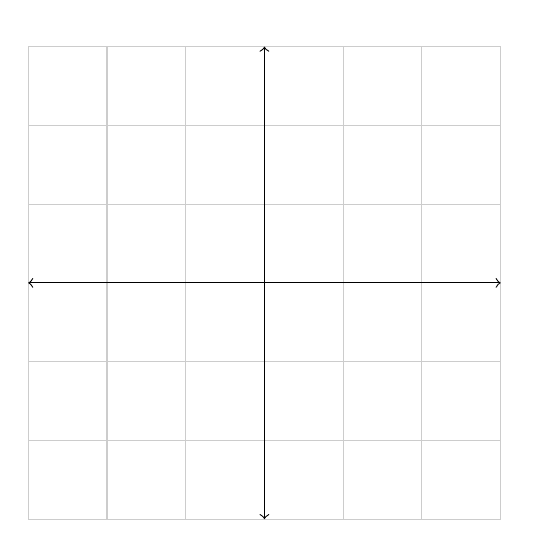
\begin{tikzpicture}
        \draw[thin,gray!40] (-3,-3) grid (3,3);
        \draw[<->] (-3,0)--(3,0) node[right]{$\RE$};
        \draw[<->] (0,-3)--(0,3) node[above]{$\IM$};
        \end{tikzpicture}
        \end{center}
        
        So, for example, let us plot a few points in the complex plane. We'll take
        \[
        z_1=1+i \qquad z_2=-1+i \qquad z_3=2-2i \qquad z_4=-2-i
        \]
        
        \begin{center}
        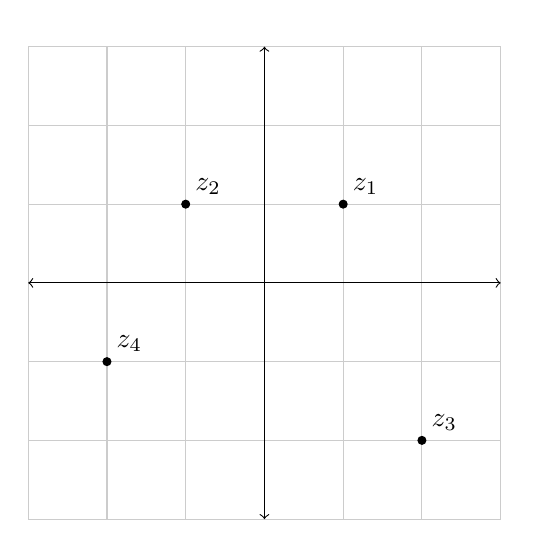
\begin{tikzpicture}
        \draw[thin,gray!40] (-3,-3) grid (3,3);
        \draw[<->] (-3,0)--(3,0) node[right]{$\RE$};
        \draw[<->] (0,-3)--(0,3) node[above]{$\IM$};
       %\addplot+[only marks] coordinates {(1,1) (-1,1) (2,-2) (-2,-1)};
        \foreach \Point/\PointLabel in {(1,1)/z_1, (-1,1)/z_2, (2,-2)/z_3, (-2,-1)/z_4}
        \draw[fill=black] \Point circle (0.05) node[above right] {$\PointLabel$};
        \end{tikzpicture}
        \end{center}
        
        Let us investigate what our algebra was doing geometrically!
        
        \noindent\textbf{Addition of complex numbers:} Recall that if we have $z_1=a_1+b_1 i$ and $z_2=a_2+b_2 i$ then
        \[
        z_1+z_2 = a_1+a_2 + (b_1 +b_2)i.
        \]
        With an explicit example, let us take
        \[
        z_1 = 1+i \qquad z_2=1-2i
        \]
        Then
        \[
        z_3=z_1+z_2=2-i.
        \]
        
        \begin{center}
        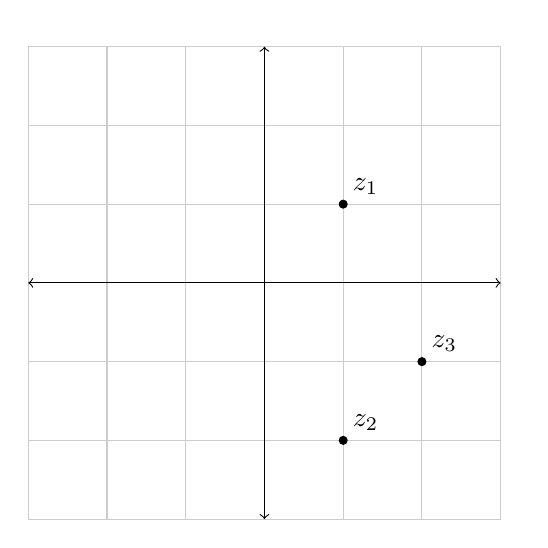
\begin{tikzpicture}
        \draw[thin,gray!40] (-3,-3) grid (3,3);
        \draw[<->] (-3,0)--(3,0) node[right]{$\RE$};
        \draw[<->] (0,-3)--(0,3) node[above]{$\IM$};
       %\addplot+[only marks] coordinates {(1,1) (-1,1) (2,-2) (-2,-1)};
        \foreach \Point/\PointLabel in {(1,1)/z_1, (1,-2)/z_2, (2,-1)/z_3}
        \draw[fill=black] \Point circle (0.05) node[above right] {$\PointLabel$};
        \end{tikzpicture}
        \quad
        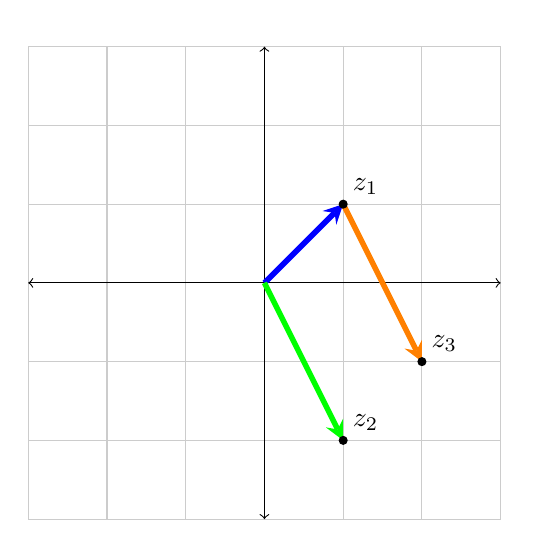
\begin{tikzpicture}
        \draw[thin,gray!40] (-3,-3) grid (3,3);
        \draw[<->] (-3,0)--(3,0) node[right]{$\RE$};
        \draw[<->] (0,-3)--(0,3) node[above]{$\IM$};
        \draw[line width=2pt,blue,-stealth](0,0)--(1,1) node[anchor=east] at (1,1){};
        \draw[line width=2pt,green,-stealth](0,0)--(1,-2) node[anchor=east] at (1,-2){};
        \draw[line width=2pt,orange,-stealth](1,1)--(2,-1) node[anchor=east] at (2,-1){};
        \foreach \Point/\PointLabel in {(1,1)/z_1, (1,-2)/z_2, (2,-1)/z_3}
        \draw[fill=black] \Point circle (0.05) node[above right] {$\PointLabel$};
        \end{tikzpicture}
        \end{center}   
        Geometrically, we arrive at $z_3$ the same way we would do vector addition in the plane $\R^2$.
        
        How about the complex conjugate? What was this doing? Given a complex number $z=a+bi$, we know that $z^*=a-bi$.  So, take the example
        \[
        z=2+2i \qquad z^*=2-2i.
        \]
        \begin{center}
        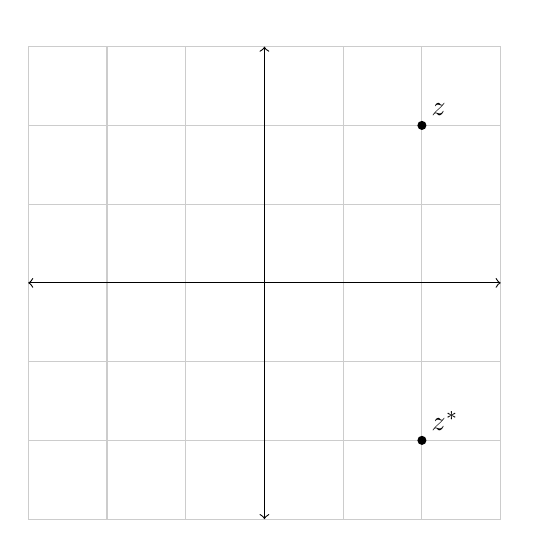
\begin{tikzpicture}
        \draw[thin,gray!40] (-3,-3) grid (3,3);
        \draw[<->] (-3,0)--(3,0) node[right]{$\RE$};
        \draw[<->] (0,-3)--(0,3) node[above]{$\IM$};
       %\addplot+[only marks] coordinates {(1,1) (-1,1) (2,-2) (-2,-1)};
        \foreach \Point/\PointLabel in {(2,2)/z, (2,-2)/z^*}
        \draw[fill=black] \Point circle (0.05) node[above right] {$\PointLabel$};
        \end{tikzpicture}
        \end{center}
        Notice that complex conjugation is just reflection about the real axis!  
        
        \section{Polar coordinates}
        An extremely important notion in planar geometry is that of \emph{polar coordinates}. Usually, we are happy to reference a point in the plane by giving the $x$-coordinates and $y$-coordinates.  In the complex case, we can give the $\RE$ and $\IM$ parts of the complex number to specify its location in the complex plane $\C$.
        
        There are many different ways you could choose to represent points in the plane, but almost all of them are rather silly to a human.  However, one that provides a great bit of intuition is polar coordinates. The idea is as follows:
        
        \begin{df}{Polar Coordinates}{pol_coord}
        \textbf{Polar coordinates} are the a coordinate system that uses $r$, the distance from the origin, and $\theta$, the counter-clockwise angle measured from the $\RE$ axis in the complex plane $\C$ (or $x$-axis in $\R^2$).
        \end{df}
        
        The following image may prove to be helpful.  
        
        \begin{center}
  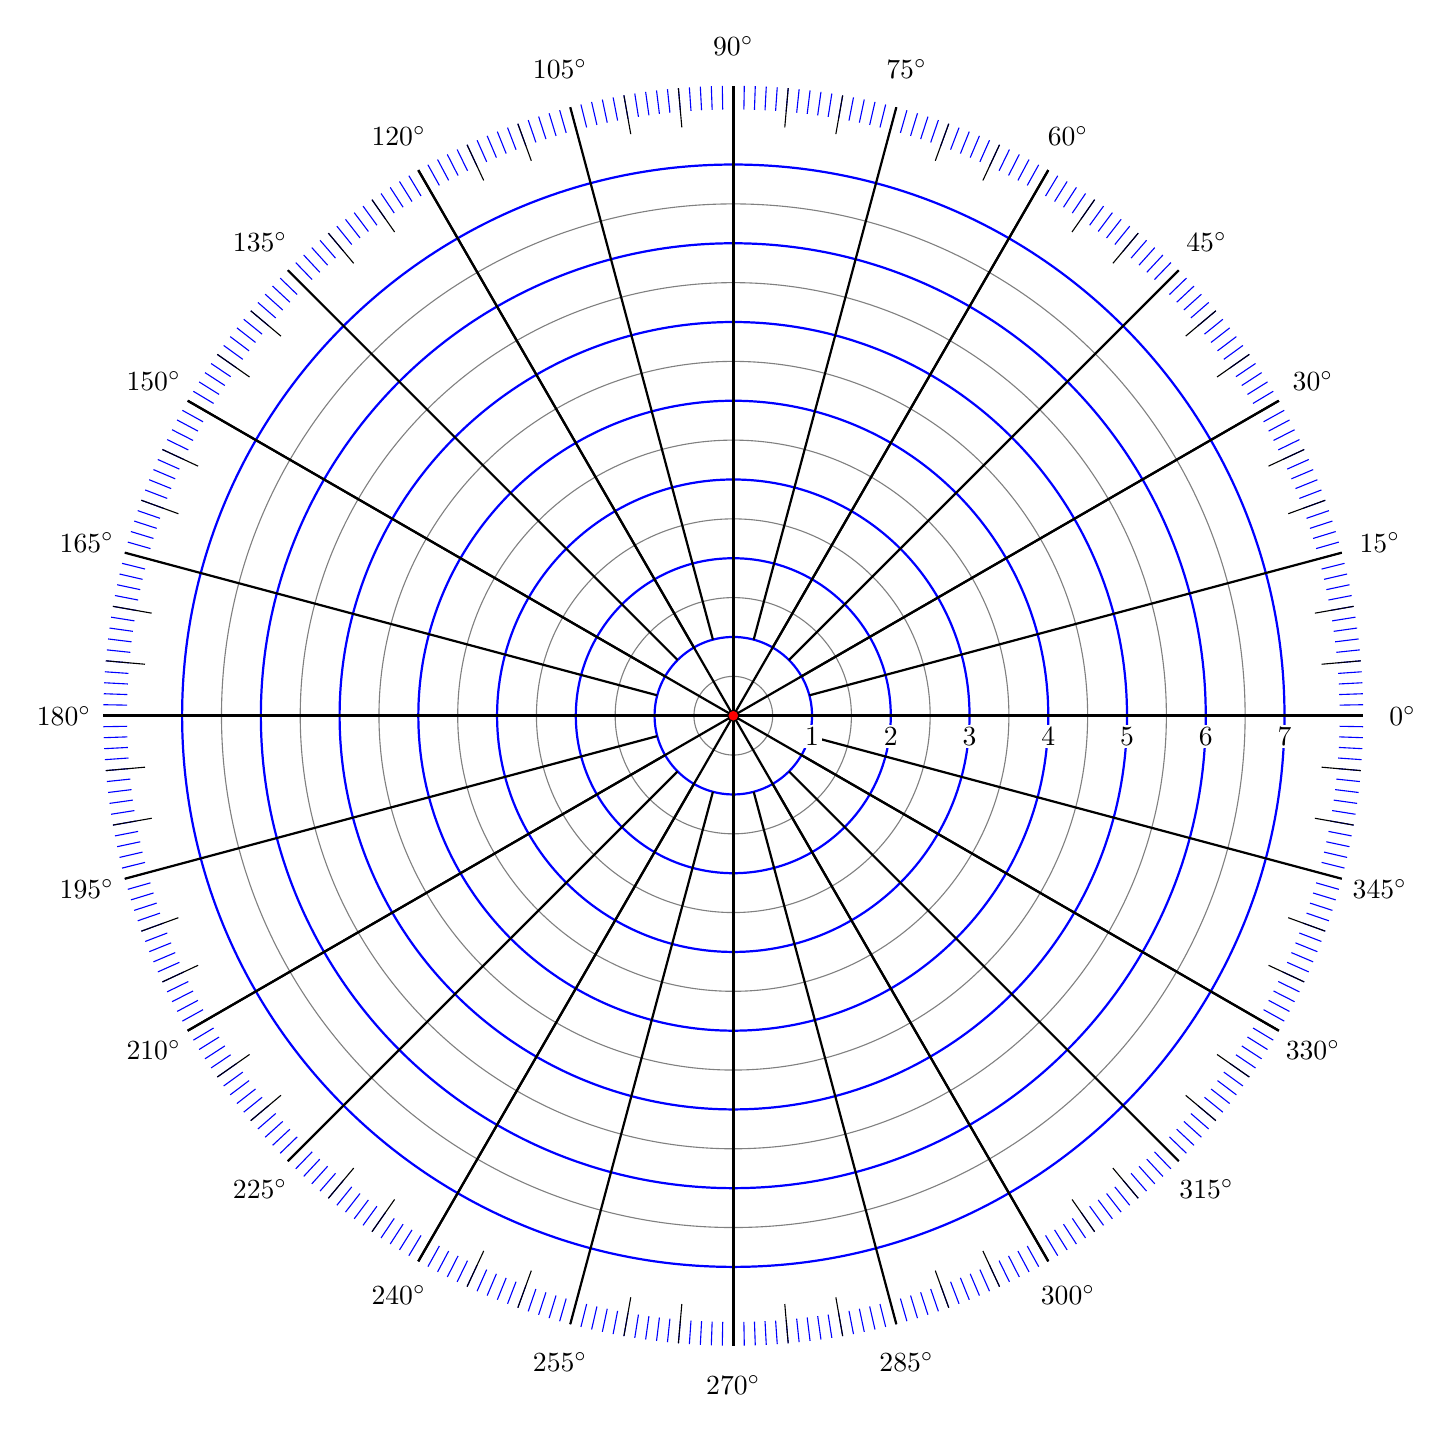
\begin{tikzpicture}
    %Circles 
    \foreach \r in {1, 2,...,7}
      \draw[blue, thick] (0,0) circle (\r);    
    \foreach \r in {0.5, 1.5,...,7}
      \draw[gray, thin] (0,0) circle (\r);
    %1° Rays
    \foreach \a in {0, 1,...,359}
      \draw[blue] (\a:7.7) -- (\a:8);
    %5° Rays
    \foreach \a in {0, 5,...,359}
      \draw[black] (\a:7.5) -- (\a:8);      
    %15° Rays
    \foreach \a in {0, 15,...,359}
      \draw[thick,black] (\a:1) -- (\a:8); 
    %30° Rays
    \foreach \a in {0, 30,...,359}
      \draw[thick,black] (0, 0) -- (\a:8);
    %Radius labels (background filled white)
    \foreach \r in {1, 2,...,7}
      \draw (\r,0) node[inner sep=1pt,below=3pt,rectangle,fill=white] {$\r$};
    %Main rays
    \foreach \a in {0, 90,...,359}
      \draw[very thick] (0, 0) -- (\a:8);
    %Angle labels  
    \foreach \a in {0, 15,...,359}
      \draw (\a: 8.5) node {$\a^\circ$};
    %Central point
    \draw[fill=red] (0,0) circle(0.7mm);
  \end{tikzpicture}
\end{center}
In this picture you can see that coordinates are given by a distance from the origin and an angle.  Of course, we remember that we tend to prefer radians, so in this case we would have
\[
0^\circ = 0 \quad 45^\circ = \frac{\pi}{4} \quad 90^\circ = \frac{\pi}{2} \quad 180^\circ = \pi.
\]

\begin{question}
        If we are given a point in cartesian coordinates (specifying a $\RE$ and $\IM$ part in $\C$ (or $(x,y)$ in $\R^2$), how can we find the polar coordinates $(r, theta)$? How about vice-versa?
\end{question}
        
        We will answer this question, but we need a bit more structure before we can get to it efficiently.
        
        \subsubsection{Taylor Series*}
        $*$ This section is not part of the class but is an extremely important concept.  Fundamentally, functions we care about can be approximated by their derivatives at a single point. For example, take the function $e^x$.  It turns out, we can write this function in a new way.  That is in the form of a \emph{power series}. In fact, we have 
        \[
        e^x = \sum_{n=0}^\infty \frac{x^n}{n!}.
        \]
        More generally, for other functions (with some sufficient conditions I don't care to get into) we can write:
        \[
        f(x)=\sum_{n=0}^\infty \frac{f^{(n)}(c)}{n!}(x-c)^n.
        \]
        The latter is known as the \textbf{Taylor series for $f$ centered at $x=c$}.
        
        You really may wonder why in the world I've just introduced this rather abstract concept, but it plays a fundamental role in the complex world.
        
        \subsubsection{Euler's Formula}
        Using the above Taylor series for $e^x$, we can plug in the following:
        \[
        e^{i\theta}=\sum_{n=0}^\infty \frac{(i\theta)^n}{n!}.
        \]
        It turns out that we find
        \[
        e^{i\theta} = \cos \theta + i \sin \theta.
        \]
        This result is known as \textbf{Euler's formula}. 
        
        \subsubsection{Polar Coordinates in $\C$}
        It turns out that Euler's formula gives us all the necessary tools to represent numbers in the complex plane in a cartesian or polar way.  
        
        \begin{df}{Modulus}{modulus}
        Given a complex number $z$, the \textbf{modulus} $\|z\|$ (think \emph{length}) of a complex number is given by
        \[
        \|z\|=\sqrt{zz^*}.
        \]
        Letting $z=a+bi$ we find
        \[
        \|z\|=\sqrt{a^2+b^2},
        \]
        which is not entirely shocking.  Just like the lengths of vectors in the plane, the ``length" of a complex number follows suit.
        \end{df}
        
        \begin{question}
                Given any $\theta$, what is the modulus of $z=e^{i\theta}$?
        \end{question}
        
        \begin{answer}
        We take
        \[
        z=e^{i\theta}=\cos \theta + i \sin \theta.
        \]
        Then
        \[
        zz^*=\cos^2 \theta + \sin^2 \theta = 1.
        \]
        So
        \[
        \|z\|=\sqrt{1}=1.
        \]
        \end{answer}
        
        It turns out that there is a fundamental relationship underlying the complex numbers.  The moral of the story is that imaginary parts of complex numbers cause rotations while the real parts cause scaling. This isn't entirely the case, but it's an alright analogy. We'll be able to uncover this as we explore polar coordinates in more depth.
        
        \subsubsection{Coordinate systems}
        \begin{remark}
        Something should be said here about the idea of coordinates in general.  Points in a plane are just that -- points.  Where they are located relative to each other is the fundamental structure whereas how we choose to measure this distance is not.  
        
        Polar coordinates are just another way of specifying where a point is located.  This choice of coordinates should not change the behavior of the algebra we have developed or any of the geometry.  Does choosing to measure an object in inches versus centimeters change the length of the object? Of course not.
        \end{remark}
        
        \section{Euler's formula and polar coordinate transformations}
        The fact that we can write
        \[
        e^{i\theta}= \cos \theta + i \sin \theta
        \]
        means that we can control the angle of a line that the complex number lives on.  Since the above function lies on the unit circle in $\C$, we can scale this with a real number to reach any point in $\C$. 
        
        That is, an equivalent way to represent a point in $\C$ is to specify its \textbf{argument} (angle, denoted $\arg(z)$) $\theta$ and its \textbf{modulus} (distance from the origin, denoted $r$ or $\|z\|$) $r$ and write
        \[
        z=re^{i\theta}.
        \]
        Before, we had always written this in a cartesian way, like
        \[
        z=a+bi.
        \]
        But we also have Euler's formula, which means that
        \[
        a+bi = re^{i\theta} = r\cos \theta + i r \sin \theta.
        \]
        This means that
        \[
        a=r\cos \theta
        \]
        and 
        \[
        b = r \sin \theta.
        \]
        You can also see that this is really nothing more than the pythagorean theorem and trigonometry the following figure.
        \begin{figure}[H]
            \centering
            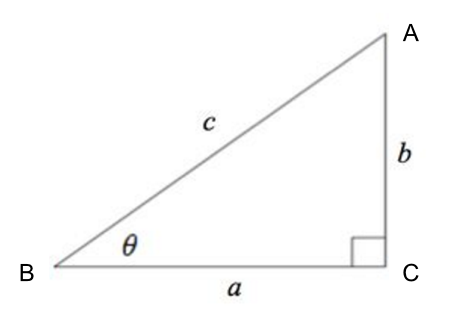
\includegraphics[width=.4\textwidth]{Figures/triangle_theta.png}
        \end{figure}
        In this case, the length of the hypotenuse ($c$ in the figure) is given by $r$. 
        
        \noindent \textbf{\textbf{Conversion from polar to cartesian:}} If you're given a point in $\C$ in polar coordinates,
        \[
        z=re^{i\theta},
        \]
        then in cartesian coordinates it will read
        \[
        z=r\cos \theta + ir\sin \theta.
        \]
        This is
        \[
        a=r\cos \theta \qquad b=r\sin \theta.
        \]
        
        \noindent \textbf{\textbf{Conversion from cartesian to polar:}} If you're given a point in $\C$ is cartesian coordinates,
        \[
        z=a+bi,
        \]
        then in polar coordinates it will read
        \[
        z=\|z\|e^{i\arctan(b/a)}.
        \]
        That is that the modulus and argument follow
        \[
        r = \|z\|=\sqrt{zz^*} \qquad \theta = \arctan\left( \frac{b}{a}\right)
        \]
        respectively. We defined $\|z\|$ to be the distance $z$ is from the origin, so this is clear.  The $\arctan(b/a)$ can be realized from the trigonometric fact that
        \[
        \tan \theta = \frac{b}{a}
        \]
        and inverting.
        
        
        \section{Multiplication of complex numbers}
        
        While we were perfectly happy to multiply complex numbers in cartesian form, it is more illuminating to multiply them in polar form.  Let us take two complex numbers
        \[
        z_1 = r_1 e^{i\theta_1} \qquad z_2 = r_2 e^{i\theta_2}.
        \]
        Then we can write the product:
        \[
        z=z_1 z_2 = (r_1 e^{i\theta_1})(r_2 e^{i\theta_2})= r_1r_2 e^{i(\theta_1+\theta_2)}.
        \]
        The thing to notice here is that the modulus of a product follows
        \[
        \|z\|=\|z_1\|\|z_2\|=r_1r_2
        \]
        and the argument of a product follows
        \[
        \arg(z)=\arg(z_1)+\arg(z_2).
        \]
        All of this is to say to the following: Multiplication of complex numbers is decomposed into rotation and scaling.
    
    
        \subsubsection{Multiplicative inverse in polar form}
        We found before that given a complex number $z$, we can find the multiplicative inverse $z^{-1}=1/z$ in cartesian form.  But this was a bit of a headache.  In polar form, however, it is much easier.  Recall that if we have
        \[
        z_1 z_2 = \left(r_1e^{i\theta_1}\right)\left(r_2e^{i\theta_2}\right)=r_1r_2e^{i(\theta_1+\theta_2)}.
        \]
        
        Now, given $z=re^{i\theta}$ we can find fairly quickly that $z^{-1}$ must be
        \[
        z^{-1}=\frac{1}{r}e^{-i\theta}.
        \]
        
        \begin{exercise}
        Show that this is indeed the multiplicative inverse.
        \end{exercise}
        
        \section{Complex functions}
        Up until now we have just looked at complex numbers themselves.  But, just having the number structure is not so interesting.  We want to investigate a bit of functions of complex numbers.  That is, functions of the form
        \[
        f\colon \C \to \C.
        \]
        These are functions that have a complex number as an input and a complex number as an output. 
        
        \begin{remark}
        Since both the input for $f$ are (essentially) 2-dimensional, we lose the ability to easily visualize these functions as we do in the case of real numbers.  We are then forced to rely more on the algebra.
        \end{remark}
        
        Let us investigate a few complex functions.  
        
        \begin{ex}{Identity Function}{id_func}
        Consider the function $f\colon \C \to \C$ given by $f(z)=z$.  This function takes in a complex number and outputs the same complex number.  So, points in the plane do not move with this function.
        \end{ex}
        
        \begin{ex}{Square Function}{square_func}
        Consider now $g\colon \C \to \C$ given by $g(z)=z^2.$ It's more englightening to write $z$ in polar form with this function.  Let us see why.
        
        Take $z=re^{i\theta}$.  Then
        \[
        g(z)=z^2=\left( re^{i\theta}\right)^2=r^2e^{2i\theta}.
        \]
        We can see that the modulus of the output grows by the square of the modulus of the input.  The argument is simply doubled.  
        \end{ex}
        
        \begin{exercise}
        Take
        \[
        z_1=1+1i \qquad z_2=e^{2\pi/3} \qquad z_3=4 \qquad z_4=-3+2i 
        \]
        as inputs to the squaring function $g$ above.  Find where $g$ outputs these inputs.
        \end{exercise}
        
        There is a lot more to say about complex functions, but it takes far more tools and time than we have to spare.
        
        \section{Contours}
        One specific example of complex functions we can visualize are \textbf{contours} (or curves).  These are also very useful and we will extend the notion of contours to curves in space.
        
        What is a contour?  It is a function of the form
        \[
        \gamma \colon \R \to \C.
        \]
        That is, $\gamma$ takes in a real number input, and outputs a complex number.  These functions look like curves in the plane.  Let's visit an example.
        
        \begin{ex}{Line Contour}{line_cont}
        Let us consider the contour
        \[
        \gamma(t)=t+it.
        \]
        Then we find that $\gamma$ looks like the $y=x$ line we write in the plane.
        
        \begin{center}
            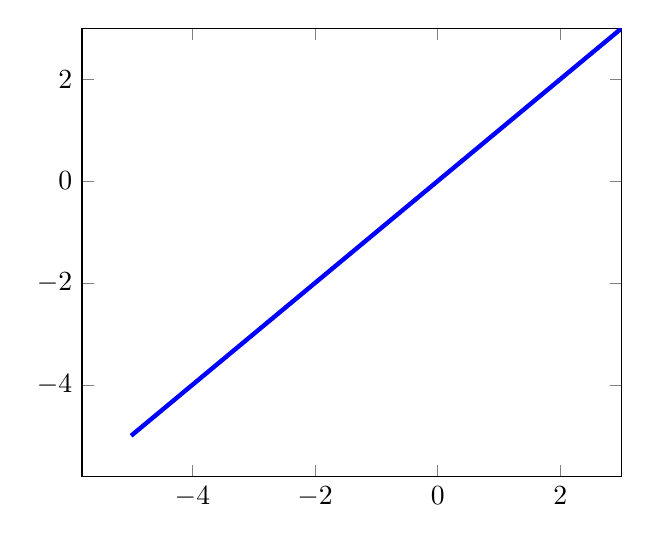
\begin{tikzpicture}
\begin{axis}[xmax=3,ymax=3, samples=50]
  \addplot[blue, ultra thick] (x,x);
\end{axis}
\end{tikzpicture}
        \end{center}
        \end{ex}
        
        \begin{ex}{Circle Contour}{circ_cont}
        Consider the contour given by
        \[
        \gamma(t)=2e^{2\pi i t}.
        \]
        Then we find that the contour is a circle with radius 2 centered at the origin.
        \begin{figure}[H]
            \centering
            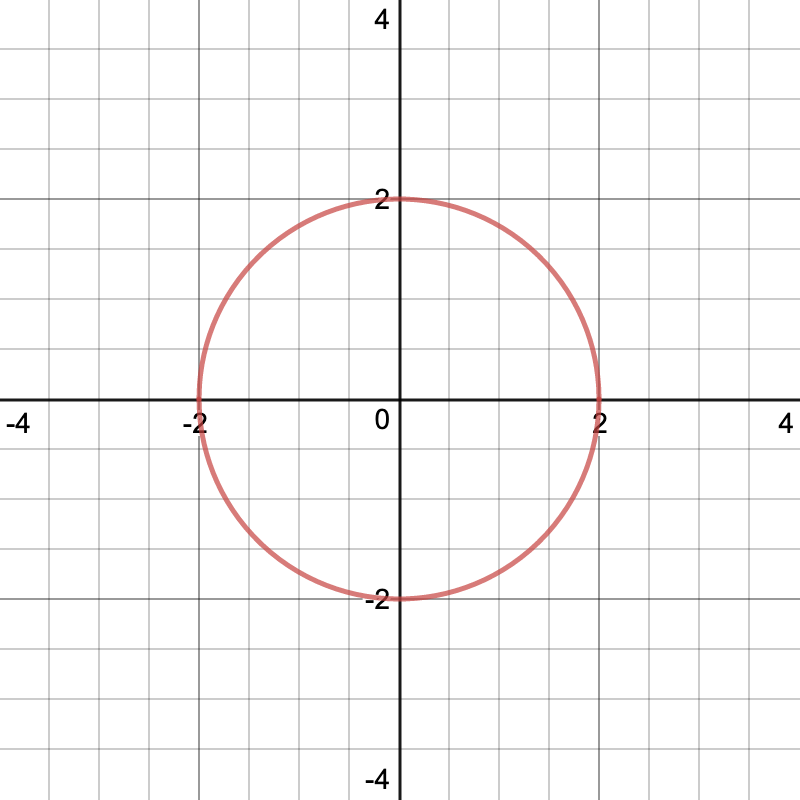
\includegraphics[width=.4\textwidth]{Figures/circle_r2.png}
        \end{figure}
        \end{ex}
        
        Up to this point, we have not really done any calculus.  But this will change now! We can ask a few questions about contours.  One in particular is the \textbf{velocity} $\gamma'(t)$ at a point in time $t$.  The other question we will look at has to do with adding up function values along a contour in the form of a \textbf{contour integral}.  These ideas will extend to higher dimensions nicely.  
        
        \section{Derivatives of contours}
        
        \begin{df}{Velocity of a Contour}{vel_cont}
        The \textbf{velocity} (or \textbf{tangent}) at time $t$ to a contour $\gamma \colon [a,b] \to \C$ is $\gamma'(t)$. That is,
        \[
        \gamma'(t)=\frac{d\gamma}{dt}=\lim_{\delta\to 0} \frac{\gamma(t+\delta)-\gamma(t)}{\delta}.
        \]
        \end{df}
        
        \begin{ex}{Velocity on a Line}{vel_on_line}
        If we take $\gamma \colon \R \to \C$ given by
        \[
        \gamma(t)=t+it,
        \]
        then the tangent is
        \begin{align*}
        \gamma'(t)&=\lim_{\delta \to 0} \frac{\gamma(t+\delta)-\gamma(t)}{\delta}\\
        &=\lim_{\delta \to 0} \frac{(t+\delta)+(t+\delta)i-t-it}{\delta}\\
        &= \lim_{\delta \to 0} \frac{\delta + i\delta}{\delta}\\
        &= 1+i.
        \end{align*}
        Doing this limit isn't necessary each time.  Instead, you should use the derivative rules you already know to do this.  You just have to do this in two parts and use the \emph{sum rule} and \emph{constant multiple rule} for derivatives in this case. 
        
        Take
        \[
        \frac{d}{dt}(t+it)=\frac{d}{dt}(t)+i\frac{d}{dt}(t)=1+i.
        \]
        \end{ex}
        
        \begin{ex}{Velocity on a Circle}{vel_on_circ}
        Consider the contour $\gamma \colon [0,1] \to \C$ given by
        \[
        \gamma(t)=2e^{2\pi i t}.
        \]
        You can imagine this as a particle orbiting a mass placed at the origin.  Then the velocity at a time $t$ is
        \[
        \gamma'(t)=4\pi i e^{2\pi i t}. 
        \]
        We can in fact find the \emph{acceleration} if we'd like.  Just take
        \[
        \gamma''(t)=-8\pi^2 e^{2\pi i t}.
        \]
        Just as a sanity check, you can check this against the centripetal acceleration magnitude you see in a physics course which is
        \[
        a=\frac{v^2}{r}.
        \]
        Here we find
        \[
        \frac{v^2}{r}=\frac{(4\pi i )^2}{2}=-8\pi^2=a.
        \]
        \end{ex}
        
        \begin{exercise}
        Draw the circle contour and draw the velocity and acceleration at the points $t=0$, $t=1/4$, $t=1/2$, and $t=3/4$. 
        \end{exercise}
        
        \section{Integration of contours}
        Many times we choose contours since we only care about a particle traveling through a region.  We just saw how we can find the velocity of the particle, but if we want to ``add up" the values of a complex valued function $f\colon \C \to \C$ we need to have some notion of integration.
        
        \begin{df}{Contour Integral}{cont_int}
        Given a complex function $f\colon \C \to \C$ and a contour $\gamma \colon [a,b] \to \C$, the \textbf{contour integral of $f$} is
        \[
        \int_\gamma f(\gamma)d\gamma.
        \]
        Now, $\gamma$ is a function of $t$, and we can write using a change of variables
        \[
        \int_\gamma f(\gamma)d\gamma = \int_a^b f(\gamma(t))\gamma'(t)dt.
        \]
        This is now something we know how to integrate.
        \end{df}
        
        \begin{ex}{Contour Integral on a Line}{cont_int_on_line}
        Let $f(z)=2+i$ and $\gamma(t)=t+it$.  Then we can integrate this contour from $t=0$ to $t=1$ by
        \begin{align*}
        \int_\gamma f(\gamma)d\gamma &= \int_0^1 f(t+it)(1+i)dt\\
        &= \int_0^1 (2+i)(1+i)dt\\
        &=(1+3i)\int_0^1 dt\\
        &=(1+3i).
        \end{align*}
        \end{ex}
        
        \begin{ex}{Contour Integral on a Circle}{cont_int_on_circ}
        Let $f(z)=z^2$ and $\gamma(t)=e^{2\pi i t}$. Then we can integrate this contour from $t=0$ to $t=1$ by
        \begin{align*}
            \int_\gamma f(\gamma)d\gamma &= \int_0^1 f\left(e^{2\pi i t}\right) (2\pi i)dt\\
            &= 2\pi i \int_0^1 \left(e^{2\pi i t}\right)^2 dt\\
            &= 2\pi i \int_0^1 e^{4\pi i t} dt.
        \end{align*}
        Here we need to use a substitution that $u=4\pi i t$ and $du=4\pi i dt$ which gives us that $u=0$ when $t=0$ and $u=4\pi i$ when $t=1$
        \begin{align*}
            \int_\gamma f(\gamma)d\gamma &= \frac{1}{2}\int_0^{4\pi i} e^u du\\
            &= \frac{1}{2} \left[ e^u \right]_0^{4\pi i}=0.
        \end{align*}
        This is zero since
        \[
        e^{4\pi i t}=e^0=1.
        \]
        \end{ex}
        
        \begin{exercise}
        Let $f(z)=z^2$ and $\gamma(t)=1+it^2$.  Then evaluate the contour integral from $t=0$ to $t=1$.
        \end{exercise}
        
        
        \chapter{Multivariable Functions}
        
        \section{Overview of multivariate functions}
        Now that we have covered enough of the complex numbers, we will move back into the vector space $\R^n$ and analyze the types of functions we can have with this space.  Specifically, we will concentrate on $\R^3$ (or $\R^2$) and functions of the form:
        \begin{align}
            &\gamma\colon \R \to \R^3\\
            &f\colon \R^3 \to \R\\
            &\mathbf{v}\colon \R^3 \to \R^3.
        \end{align}
        Abstractly, I could call each one of these functions a \emph{field} (in the physics sense).  However, I'll refrain from this (and let the mathematicians breathe a sigh of relief).
        
        
        \begin{enumerate}[(1)]
        \item Functions of the form
        \[
        \gamma \colon \R\to \R^3
        \]
        are \textbf{curves}.  Often times, we will have 
        \[
        \gamma \colon [a,b]\to \R^3
        \]
        when we want curves with specific endpoints. We will concentrate first on curves, so I'll save the extra detail for a bit later.
        
        \item Functions of the form
        \[
        f\colon \R^3 \to \R
        \]
        are \textbf{scalar fields} or \textbf{scalar functions}.   These functions are useful in describing quantities like temperature in space.  At each point in space $\R^3$, we can assign a single number $\R$ that tells us this temperature.  One may ask how this function changes from point to point.  Asking this question sends you immediately to investigating the \emph{gradient}.  It turns out, using our temperature example, that we can understand heat flow by understanding temperature gradients.
        
        \item Functions of the form
        \[
        \mathbf{v}\colon \R^3 \to \R^3
        \]
        are called \textbf{vector fields}.  Roughly speaking, at each point in space $\R^3$, we can place a vector that is also in $\R^3$.  These fields are very important in describing systems that have flow.  For example, fluid flow or electromagnetism are vector field theories.  What will it mean to find the change in a vector field?  This will lead us to the notion of the \emph{total derivative}.  This concept is a bit abstract at first but will really tell us the proper notion of the derivative.
        \end{enumerate}
        
        \section{Curves in space}
        
        We will begin these multivariate functions by considering functions that are not multivariate!  Why? Because curves are very much useful tools and this will help us visualize results for the other types of functions.
        
        Let us consider a curve
        \[
        \gamma \colon \R \to \R^3.
        \]
        We will specify a specific curve by supplying three functions $f_1(t)$, $f_2(t)$, and $f_3(t)$. Specifically, each of these functions $f_i$ is a function $f_i\colon \R \to \R$. Then, we can say that
        \[
        \gamma(t)=(f_1(t),f_2(t),f_3(t))=\begin{bmatrix} f_1(t)\\ f_2(t)\\ f_3(t)\end{bmatrix}.
        \]
        \emph{Note, I will likely use these above notations for vectors interchangeably.} 
        
        Each $f_i(t)$ (for the values $i=1,2,3$) is called a \textbf{coordinate function}.  Intuitively, the coordinate function tells us where the curve is at a time $t$. That is
        \begin{align*}
            &f_1(t) \quad \textrm{the $x$-position of $\gamma$ at time $t$,}\\
            &f_2(t) \quad \textrm{the $y$-position of $\gamma$ at time $t$,}\\
            &f_3(t) \quad \textrm{the $z$-position of $\gamma$ at time $t$.}
        \end{align*}
        The nice thing about these coordinate functions is we entirely know how to deal with their calculus since each is a function $f_i\colon \R \to \R$.
        
        Now, we can find the \textbf{tangent vector} or \textbf{velocity vector} to the curve $\gamma$ at a time $t$.  We covered this in the complex case, and the idea here is arguably more straightforward. 
        
        Imagine that $\gamma(t)$ is the position of a small particle at the time $t$.  Then the velocity is the time rate of change of this position.  Specifically, we see how each of the coordinate functions changes, and this will tell us how the position changes! So, we have the following.
        
        \begin{df}{Tangent Vector to a Curve}{tang_to_curve}
        Given a curve $\gamma$, the \textbf{tangent vector to $\gamma$ at the time $t$} is
        \[
        \gamma'(t)=\lim_{\delta \to 0} \frac{\gamma(t+\delta)-\gamma(t)}{\delta}.
        \]
        It turns out that we find $\gamma'$ is
        \[
        \gamma'(t)=(f_1'(t),f_2'(t),f_3'(t))=\begin{bmatrix} f_1'(t)\\ f_2'(t)\\ f_3'(t)\end{bmatrix}.
        \]
        \end{df}
        
        \begin{ex}{Graph of a Quadratic Function}{graph_quad}
        Consider the curve $\gamma\colon \R \to \R^2$ given by
        \[
        \gamma(t)=(t,t^2).
        \]
        This curve looks exactly like the graph of the function $f(x)=x^2$ that we have drawn many times before. 
        \begin{figure}[H]
            \centering
            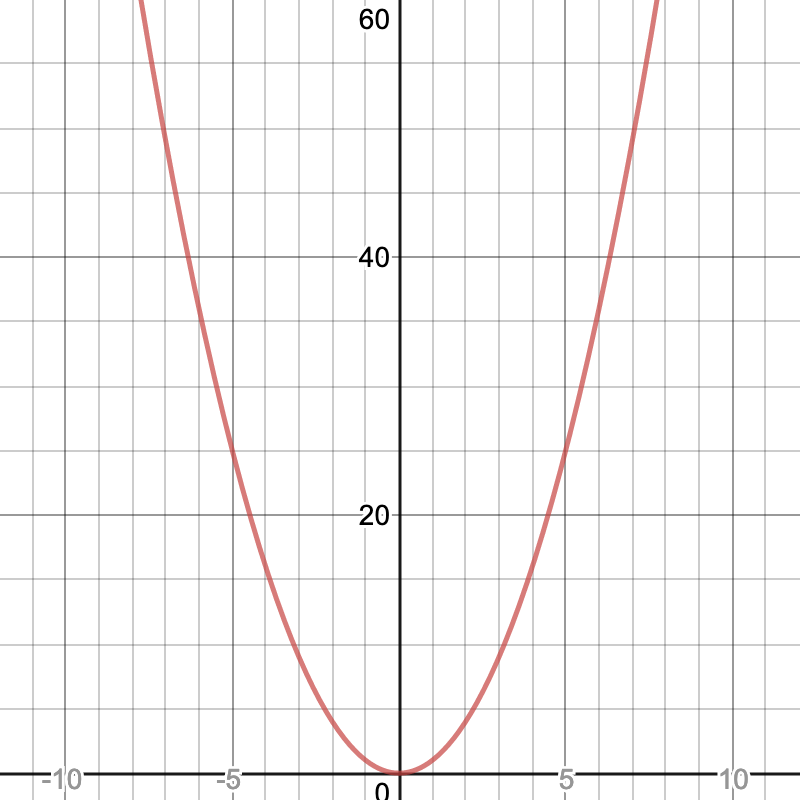
\includegraphics[width=.4\textwidth]{Figures/quadratic_curve.png}
        \end{figure}
        
        What is the tangent vector at time $t$? We have
        \[
        \gamma'(t)=(1,2t).
        \]
        If we take this $y$-value over the $x$-value we arrive at the same conclusion for the derivative to $f(x)=x^2$ (i.e., $f'(x)=2x$).
        \end{ex}
        
        \begin{ex}{Circle Curve}{circ_curve}
        Consider the curve $\gamma \colon [0,1] \to \R^2$ given by
        \[
        \gamma(t)=(\cos (2\pi t),\sin (2\pi t)).
        \]
        This curve is a circle of radius $1$ centered at $(0,0)$.  We can find the tangent vector at a time $t$ by
        \[
        \gamma'(t)=(-2\pi \sin(2\pi t), 2\pi \cos(2\pi t)).
        \]
        See the following graphs
        
    \begin{figure}[H]
    \centering
    \begin{subfigure}[h]{0.45\textwidth}
        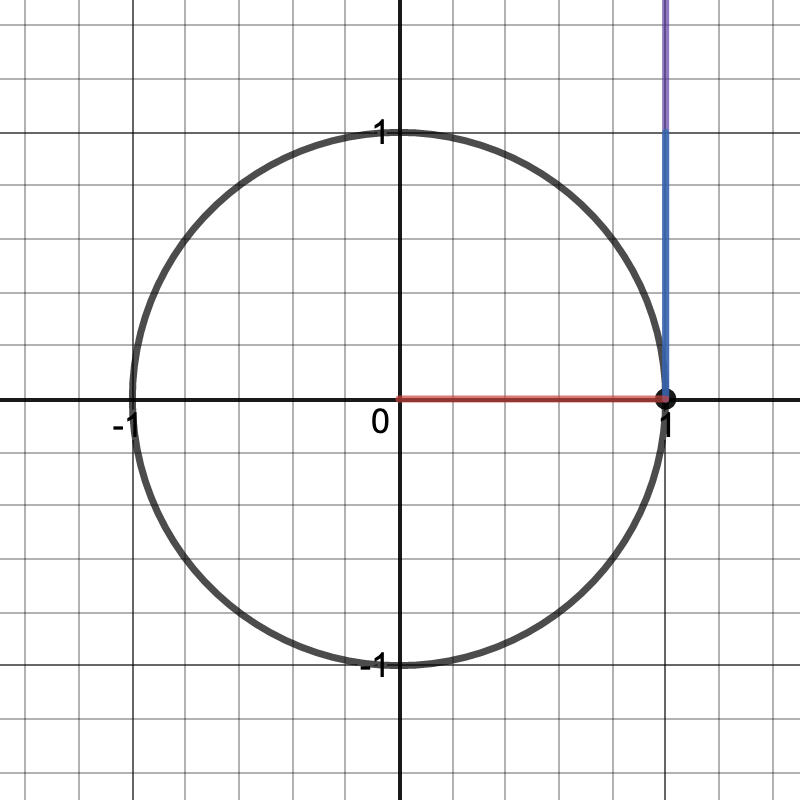
\includegraphics[width=\textwidth]{Figures/circ_tang_1.png}
        \caption{Tangent vector at $t=0$.}
    \end{subfigure}
    ~ 
    \begin{subfigure}[h]{0.45\textwidth}
        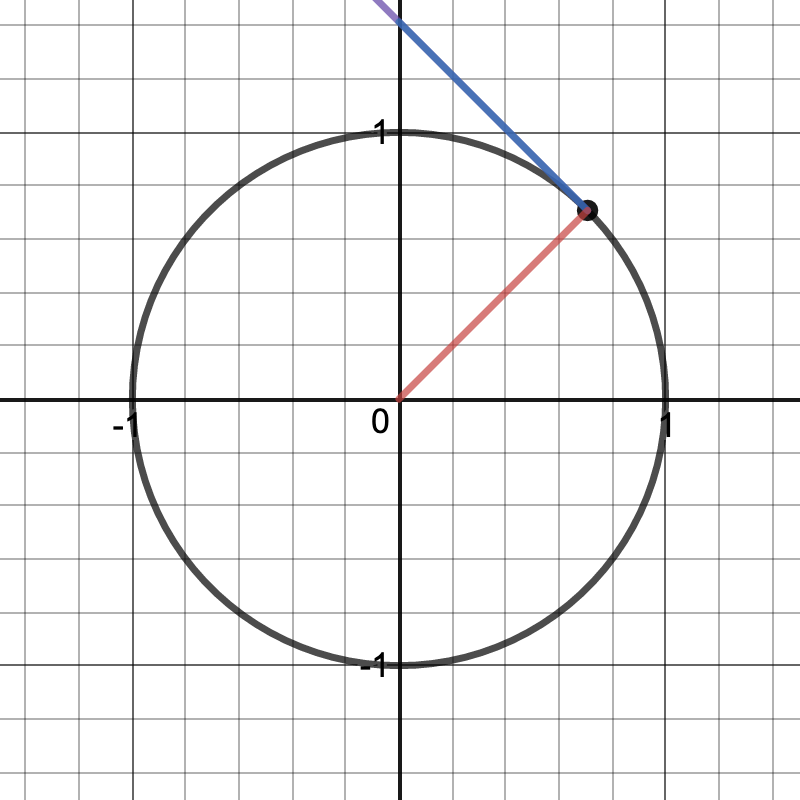
\includegraphics[width=\textwidth]{Figures/circ_tang_2.png}
        \caption{Tangent vector at $t=\frac{1}{8}$.}
    \end{subfigure}
    
    \begin{subfigure}[h]{0.45\textwidth}
        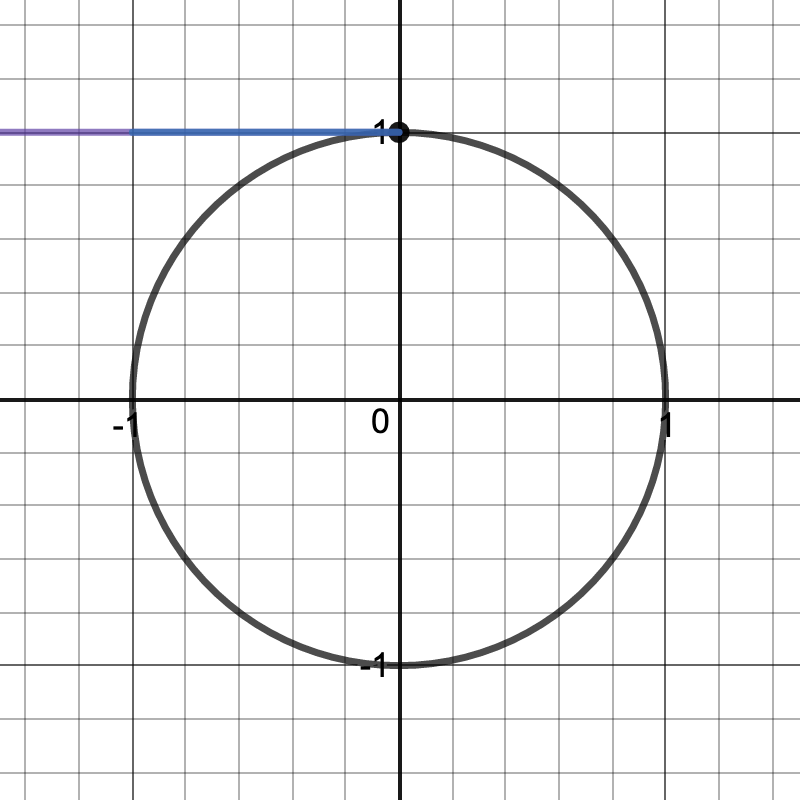
\includegraphics[width=\textwidth]{Figures/circ_tang_3.png}
        \caption{Tangent vector at $t=\frac{1}{4}$.}
    \end{subfigure}
    ~
    \begin{subfigure}[h]{0.45\textwidth}
        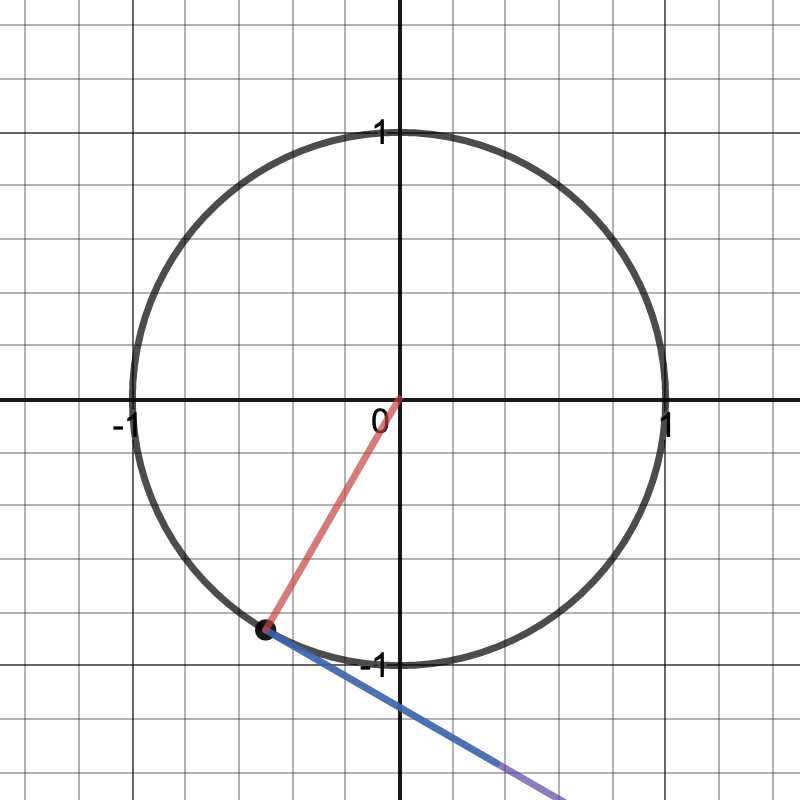
\includegraphics[width=\textwidth]{Figures/circ_tang_4.png}
        \caption{Tangent vector at $t=\frac{2}{3}$.}
    \end{subfigure}
        \end{figure}
        
        We can also compute the \textbf{normal vector} or \textbf{acceleration vector} to a curve by taking another derivative.  We write
        \[
        \gamma''(t)=(-4\pi^2 \cos(2\pi t),-4\pi^2 \sin(2\pi t)).
        \]
        \end{ex}
        
        \subsubsection{Line integrals}
        
        In reality, we like to add up function values along curves.  We have already done this before in the complex case with contours.  You also did this in a calculus I course via the Riemann integral.  We will get to this, but we need to know the correct functions to add up along a curve first. These will be the vector and scalar fields fields.
        
        
        
        \section{Scalar fields}
        The next major class of functions we will consider are the scalar fields.  That is, functions that take the form
        \[
        f\colon \R^3 \to \R.
        \]
        Often, it will be helpful to visualize functions by considering instead
        \[
        f\colon \R^2 \to \R
        \]
        and looking at the \emph{graph} of $f$.  
        
        \begin{ex}{Graph of a function}{graph_of_func}
        Whenever we talk of a function of the form
        \[
        f\colon \R \to \R
        \]
        we inherently tend to draw the graph of the function $f$.  By graph, I mean that given $f$, we usually just draw $(x,f(x))$ in the plane.
        
        Take for example, $f\colon \R \to \R$ given by $f(x)=x^2$.  We usually draw the plane $\R^2$ and graph the curve $(x,f(x))$ which looks like
        \begin{figure}[H]
            \centering
            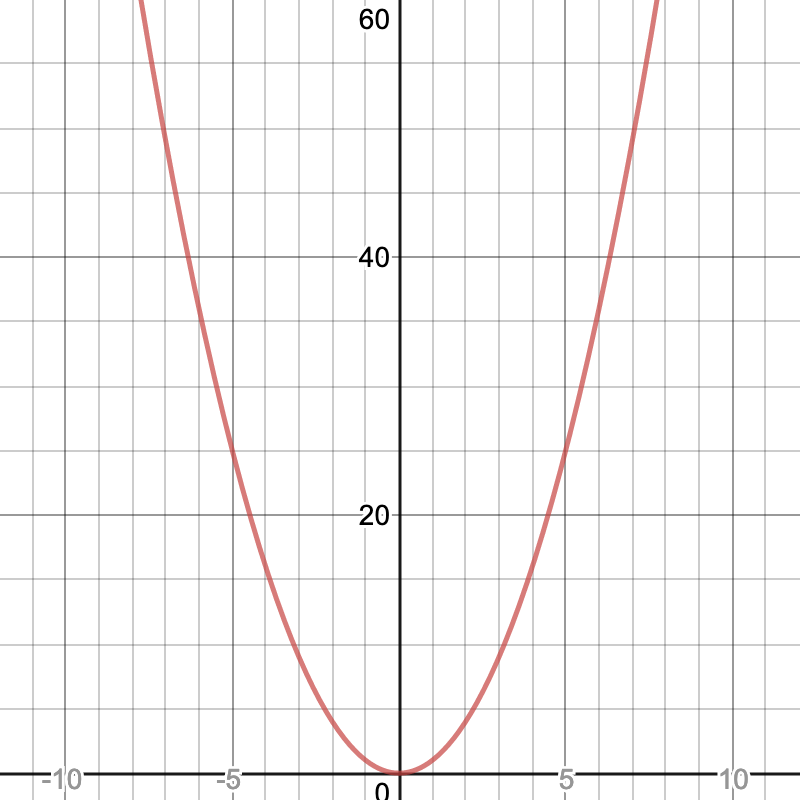
\includegraphics[width=.5\textwidth]{Figures/quadratic_curve.png}           
        \end{figure}
        All of this is to say that graphs of these types of functions are special kinds of curves.  In other words, they are curves that pass the vertical line test.
        \end{ex}
        
        \begin{ex}{The Paraboloid}{paraboloid}
        Let $f\colon \R^2 \to \R$ be given by
        \[
        f(x,y)=x^2+y^2.
        \]
        We can plot the graph of the function by plotting $(x,y, f(x,y))$ in $\R^3$.  This will look like:
        \begin{figure}[H]
            \centering
            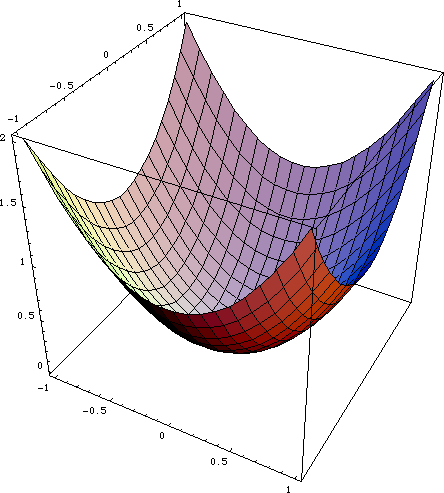
\includegraphics[width=.4\textwidth]{Figures/paraboloid.png}
        \end{figure}
        Then we can analyze this function in a few nice ways.  
        
        If we fix a value for $x$ or $y$, then we will be able to look at $f$ as a function of just a single variable.  
        \begin{itemize}
        \item So we can, for example, fix $y=0$ and then we have
        \[
        f(x,0)=x^2.
        \]
        So along the $y=0$ line, the function is just the parabola we are used to! 
        
        \item Similarly, we can force $x=0$ and arrive at
        \[
        f(0,y)=y^2
        \]
        is also a parabola.  
        
        \item But we are not limited to these choices.  We could have chosen $y=5$ and we would have
        \[
        f(x,5)=x^2+25
        \]
        which is a parabola shifted upwards by 25 units.
        
        \item  Again, we could also choose yet another ``slice" of this function and let $x=y$ which would give us
        \[
        f(x,x)=x^2+x^2=2x^2.
        \]
        So, along the $x=y$ line, the parabola is scaled by 2.
        
        \item One other method of analyzing this function would be to find what the \textbf{level curves} of this function are.  What are the points $(x,y)$ that satisfy $f(x,y)=c$?  We call these level curves much in the way that a topographical map plots curves along the areas with equal height.  For this example, consider the set of points $(x,y)$ so that $f(x,y)=1.$ This means
        \[
        f(x,y)=1=x^2+y^2.
        \]
        Since we have
        \[
        x^2+y^2=1
        \]
        that means each level curve is a circle!
        \item Here is a ``topographical map" for this function (i.e., a plot of the level curves for this paraboloid.)
        \begin{figure}[H]
            \centering
            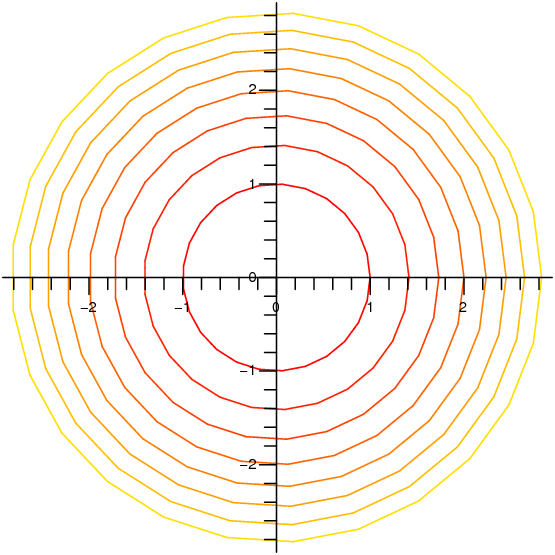
\includegraphics[width=.4\textwidth]{Figures/parabolic_level_curves.png}
        \end{figure}
        Here, each circle represents $f(x,y)=c$ for different values of $c$.  This really \emph{is} a topographical map!
        \end{itemize}
        \end{ex}
        
        \begin{exercise}[Plane]
        Repeat this analysis for yourself for the following function:
        \[
        f(x,y)=x+y.
        \]
        \end{exercise}
        
        \section{Level surfaces}
        In the planar case, we would often have to specify a set of points like
        \[
        x^2+y^2=1
        \]
        which is the circle.  
        
        In higher dimensions, we can do the same in order to visualize functions of the form $f\colon \R^3\to \R$ written as $f(x,y,z)$.  If we pick some constant $c$ and write
        \[
        f(x,y,z)=c
        \]
        then we will get the \textbf{level surfaces} for the function $f(x,y,z)$.  Visualizing functions of three variables (or more) $f(x,y,z)$ requires us to visualize in four or more dimensions. So we often reduce the problem to visualizing level surfaces.
        
        \begin{ex}{A Sphere as a Level Surface}{sphere_lev_surf}
        We can consider the following function
        \[
        f(x,y,z)=x^2+y^2+z^2.
        \]
        If we take the one level set, that is the points $(x,y,z)$ that satisfy
        \[
        x^2+y^2+z^2=1
        \]
        then we get the \emph{2-sphere}.  These are the set of points that are all a distance one from the origin.  Here is a picture:
        \begin{figure}[H]
            \centering
            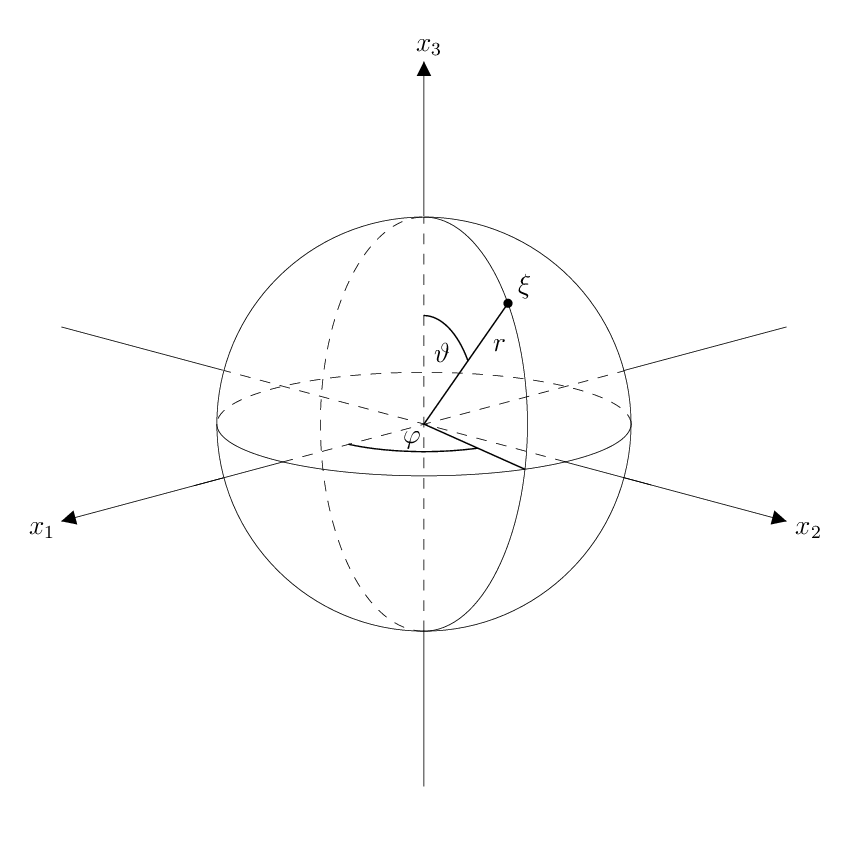
\includegraphics[width=.4\textwidth]{Figures/sphere.png}
        \end{figure}
        \end{ex}
        
        \begin{ex}{The Hyperboloids}{hyperboloids}
        Consider a family of surfaces given by the level surfaces of
        \[
        f(x,y,z)=x^2+y^2-z^2.
        \]
        \begin{itemize}
            \item If we take $c=0$ and set
            \[
            x^2+y^2-z^2=0.
            \]
            then we find the 0 level surface. In this case, we can do a bit of work to find
            \[
            z=\pm \sqrt{x^2+y^2}.
            \]
            Notice, if we pick any value for $z$, that we get a circle at that level!  When $z=0$, we get a single point.  It turns out that we get the \emph{(double) cone} surface which looks like
            \begin{figure}[H]
                \centering
             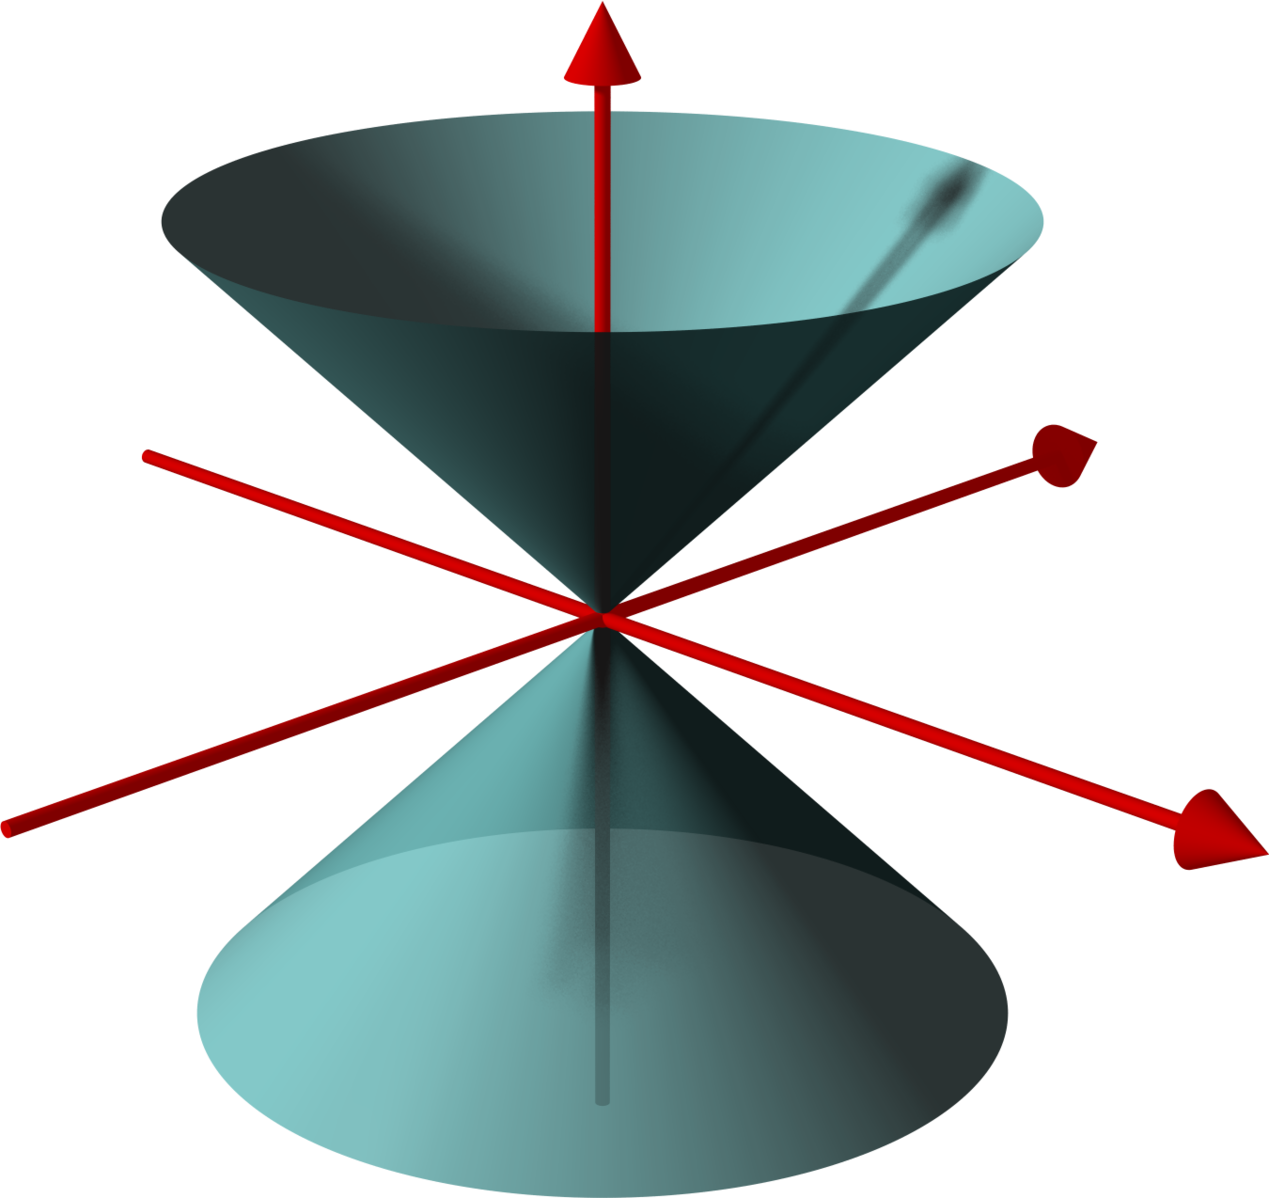
\includegraphics[width=.4\textwidth]{Figures/cone_surface.png}
            \end{figure}
            
            \item If we take $c=1$ and set
            \[
            x^2+y^2-z^2=1
            \]
            we get the \emph{hyperboloid of one sheet}.  This looks like
            \begin{figure}[H]
                \centering
                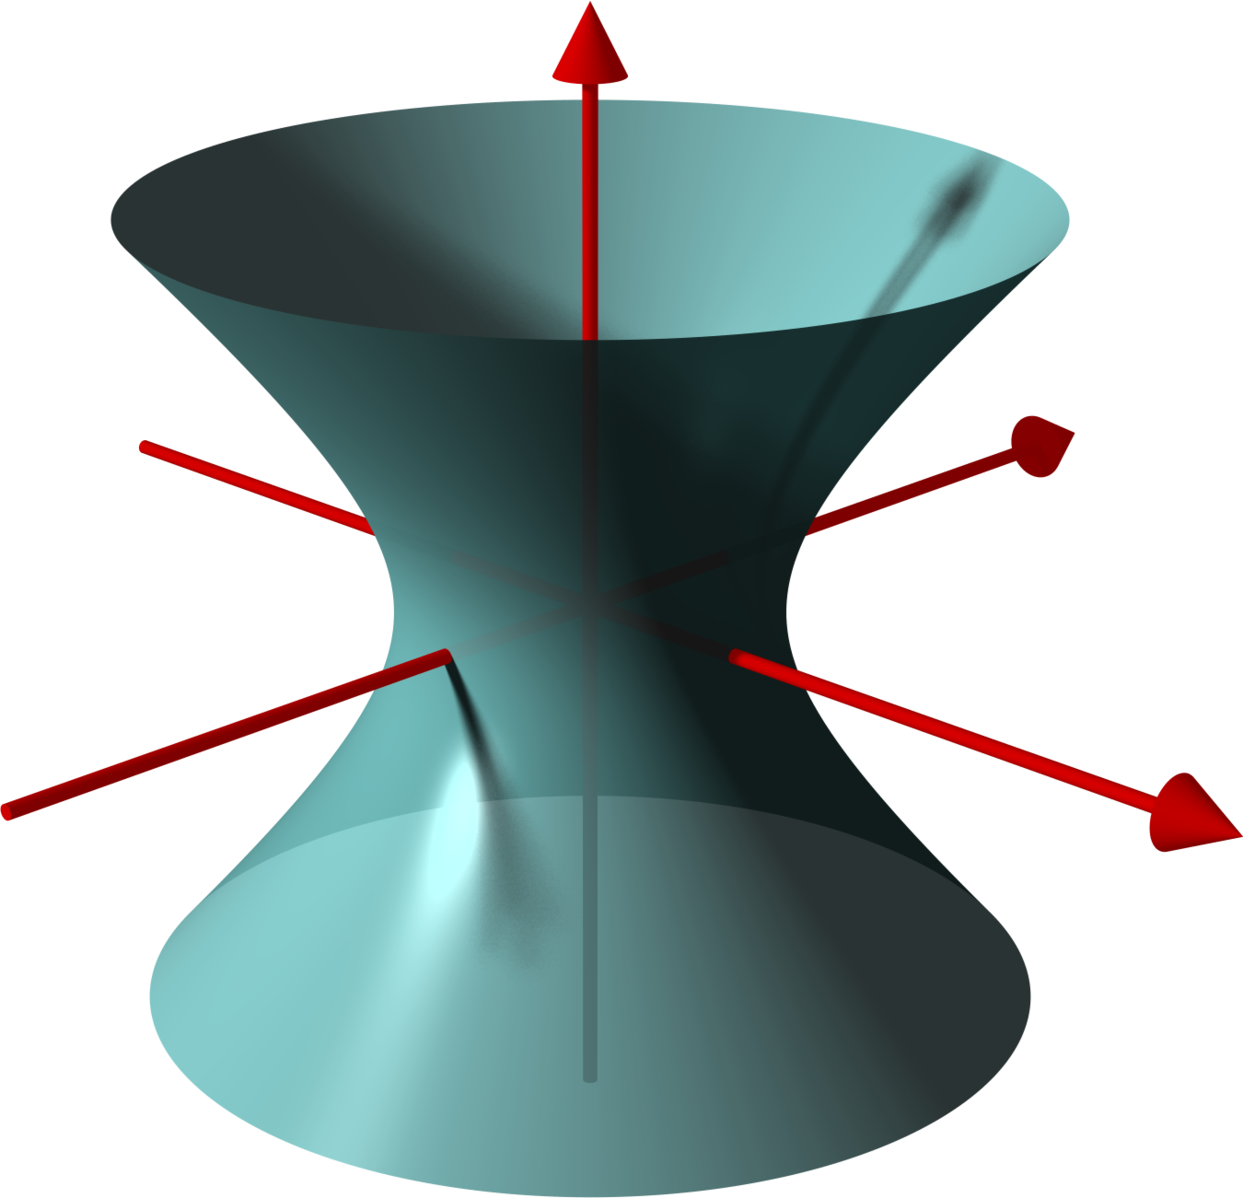
\includegraphics[width=.4\textwidth]{Figures/hyperboloid_1_sheet.png}
            \end{figure}
            
            \item If we take $c=-1$ and set
            \[
            x^2+y^2-z^2=-1
            \]
            we get the \emph{hyperboloid of two sheets}.  This looks like
            \begin{figure}[H]
                \centering
                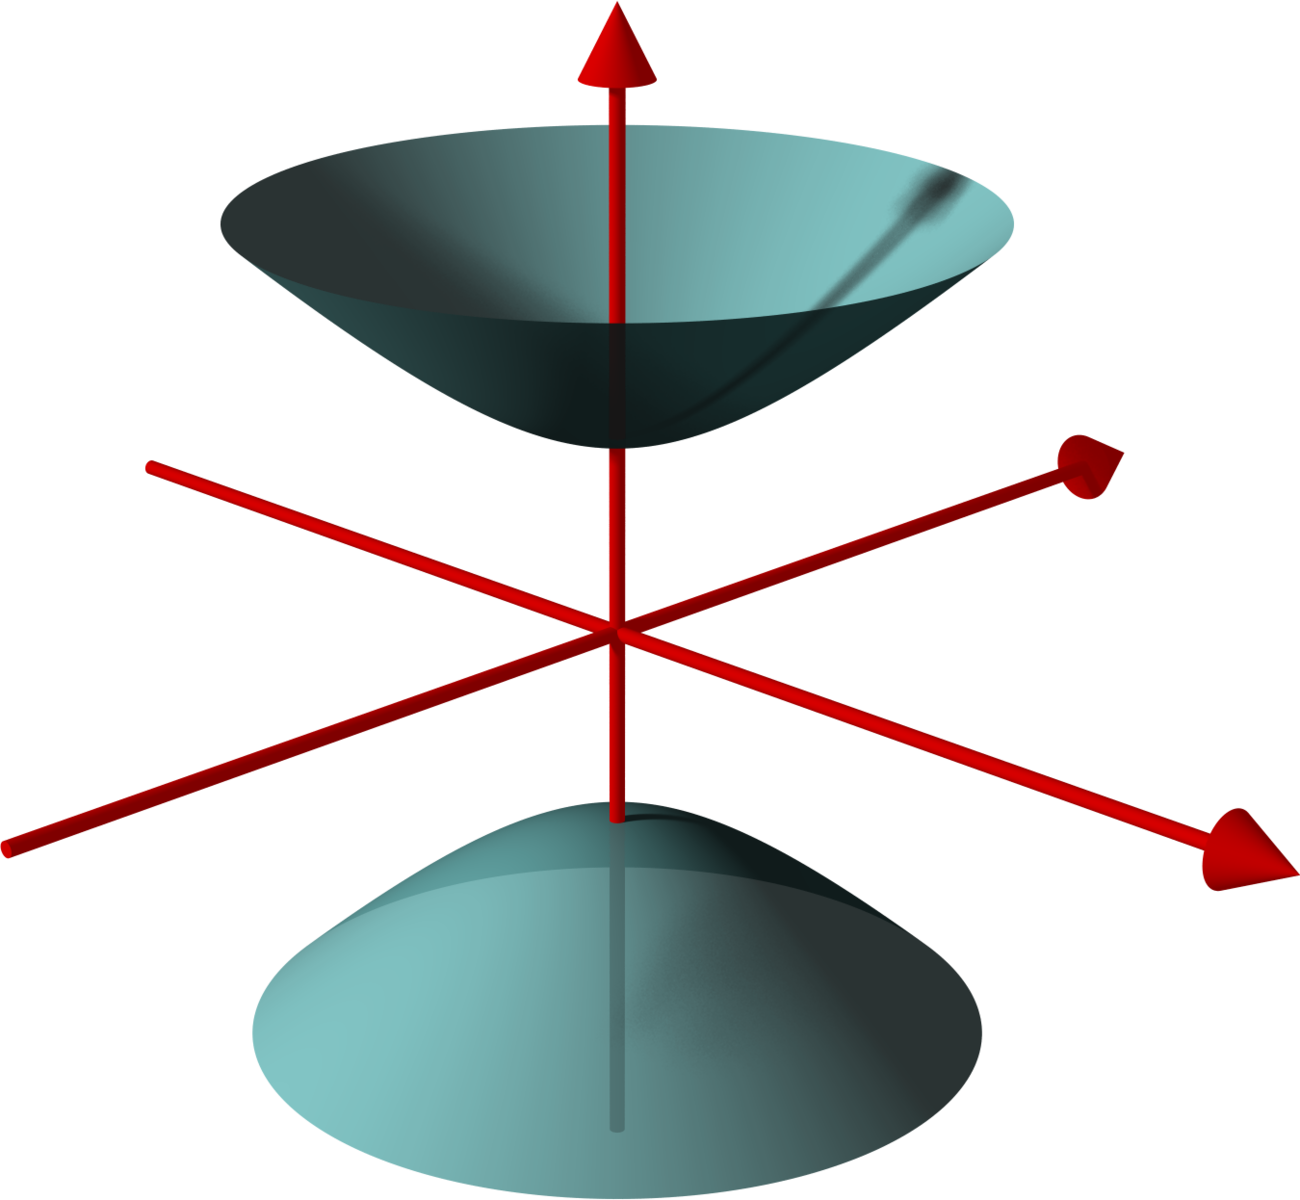
\includegraphics[width=.4\textwidth]{Figures/hyperboloid_2_sheet.png}
            \end{figure}
        \end{itemize}
        \end{ex}
        
        \begin{ex}{The Torus}{torus}
        For this example, I will choose specific nice numbers, but this is a yet another case of a level surface.  Take
        \[
        \left(5-\sqrt{x^2+y^2}\right)^2+z^2=2.
        \]
        This gives us the \emph{torus} with inner radius (the radius from the center of the donut hole to the center of the tube) $5=R$ and tube radius $2=r$. This looks like
        \begin{figure}[H]
            \centering
            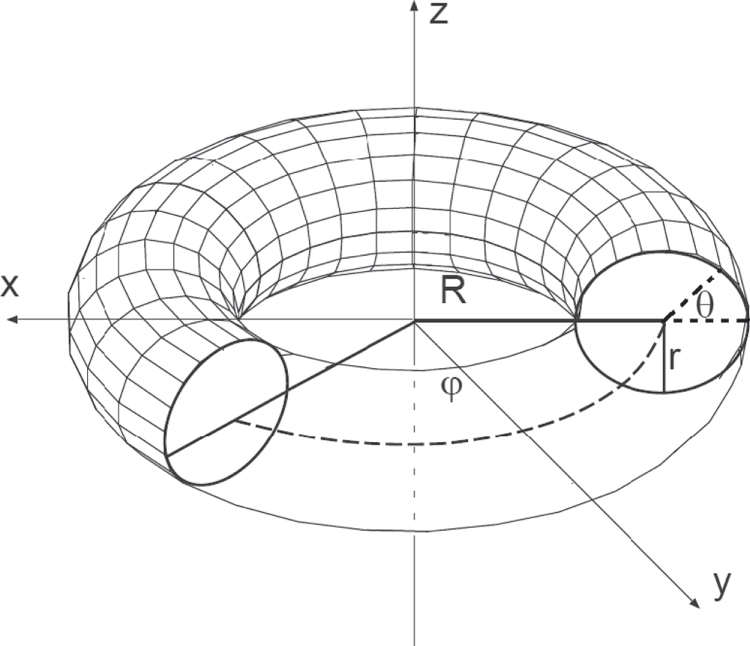
\includegraphics[width=.4\textwidth]{Figures/torus.png}
        \end{figure}
        \end{ex}
        
        
        We have given ourselves ways of understanding the scalar functions and curves, but still need to develop a manner to understand vector fields.  We will not only need to understand vector fields in their own right, but we will need them in order to investigate how the scalar fields change from point to point.  Roughly speaking, the ``derivative" of a scalar field will be a vector field.
        
        \section{Vector Fields}
        
        A vector field is a function that inputs a vector and outputs a vector. Specifically, we can write
        \[
        \mathbf{v}(x,y,z)=(f_1(x,y,z),f_2(x,y,z),f_3(x,y,z))=\begin{bmatrix} f_1(x,y,z)\\ f_2(x,y,z) \\ f_3(x,y,z)\end{bmatrix}.
        \]
        Notice the differences and similarities between vector fields, scalar fields, and curves.  Just as before, it will be nice to visualize many vector fields in the $xy$-plane to avoid drawing in 3-dimensions. Of course, we can use technology to make nice plots in space.
        
        Intuitively, a vector field is an assignment of a vector at each point in space.  To match this intuition we tend to just draw a collection of arrows in space.
        
        \begin{ex}{Eastward Wind}{east_wind}
        Consider the vector field
        \[
        \mathbf{v}\colon \R^2 \to \R^2
        \]
        given by
        \[
        \mathbf{v}(x,y)=(1,0).
        \]
        At each point $(x,y)$, we are assigning a vector that points a distance 1 in the $x$-direction. See the following figure.
        \begin{figure}[H]
            \centering
            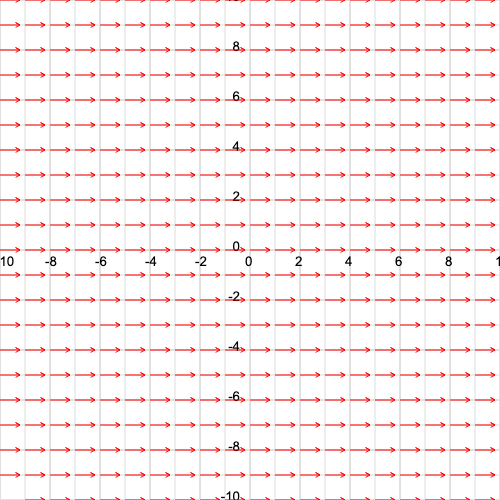
\includegraphics[width=.6\textwidth]{Figures/wind_field.png}
        \end{figure}
        \end{ex}
        
        \begin{ex}{Line Source}{line_source}
        Consider the vector field in the plane given by
        \[
        \mathbf{v}(x,y)=(x+y,x+y).
        \]
        See the following figure.
        \begin{figure}[H]
            \centering
            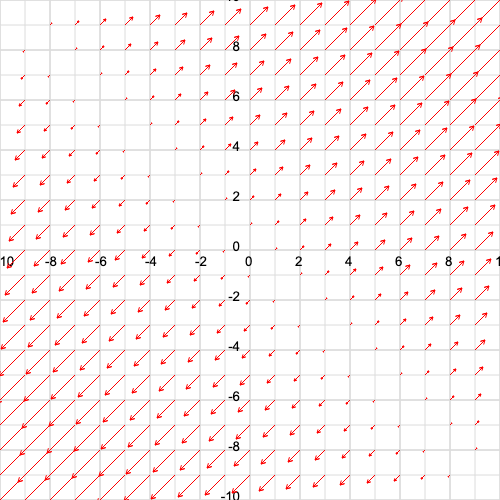
\includegraphics[width=.6\textwidth]{Figures/v_field_1.png}
        \end{figure}
        \end{ex}
        
        \begin{ex}{Whirlpool}{whirlpool}
        Consider the vector field in the plane given by
        \[
        \mathbf{v}(x,y)=(y,-x).
        \]
        See the following figure.
        \begin{figure}[H]
            \centering
            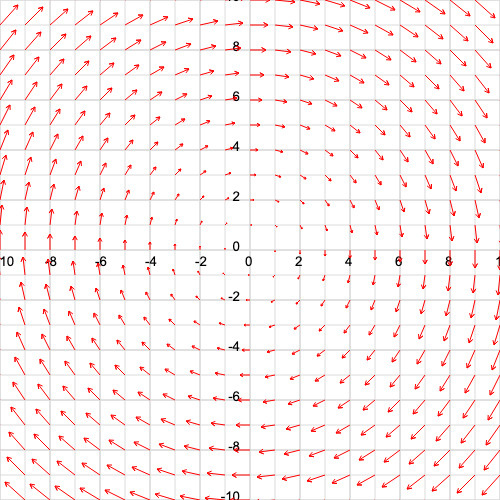
\includegraphics[width=.6\textwidth]{Figures/v_field_3.png}
        \end{figure}
        \end{ex}
        
    \chapter{Calculus with Multivariate Functions}
        
        \section{Differentiation of fields}
        One may now wonder where the calculus comes in.  We are almost there, but we should know what it means intuitively to use the calculus tools with these more general fields.
        
        Curves will prove to be a great tool in the analysis of these scalar fields.  We will also need to understand how vectors transform from point to point which will require us to recall the knowledge we gained on linear transformations.
        
        Roughly speaking, we will have:
        \begin{itemize}
            \item \textbf{Curves:} Derivatives of curves $\gamma(t)$ are vectors. Specifically, we have already seen the tangent vector $\gamma'(t)$ and acceleration vector $\gamma''(t)$.
            \item \textbf{Scalar Fields:} Derivatives of scalar fields $f(x,y,z)$ will depend on which input of the function we change.  We can collect the partial derivatives corresponding to finding derivatives in one input into a vector called the \emph{gradient}.
            \item \textbf{Vector Fields:} Derivatives of vector fields $\mathbf{v}(x,y,z)$ will require us to see how each component of $\mathbf{v}$ changes based on how each individual input changes.  In this case, this collection of derivatives will be put into a matrix known as the \emph{total derivative}.
        \end{itemize}
        
        \begin{remark}
        The important notion that we need to understand is the following.
        
        \emph{The derivative of a function at a point is the best linear approximation to the function.} 
        
        Based on this wording, it is intuitive to imagine derivatives as vectors or matrices.
        \end{remark}
        
        \section{Functions of Fields}
        In our world, we often care about combining different fields together.  For example, we can take the electric field created by a single charged particle and add this field to another field created by a different charged particle. What I mean, is we can write
        \[
        \mathbf{v}(x,y,z)+\mathbf{u}(x,y,z)
        \]
        and make sense of this.  Just as we did with vectors, we add the components together! That is if we have
        \begin{align*}
        \mathbf{v}(x,y,z)&=(f_1(x,y,z),f_2(x,y,z),f_3(x,y,z))\\ \mathbf{u}(x,y,z)&=(g_1(x,y,z),g_2(x,y,z),g_3(x,y,z)),
        \end{align*}
        then
        \[
        \mathbf{v}(x,y,z)+\mathbf{u}(x,y,z)=(f_1+g_1,f_2+g_2,f_3+g_3).
        \]
        Intuitively, this just adds together the vectors at each point!
        
        \begin{ex}{Addition of vector fields}{add_vect_fields}
        Consider the following vector fields
        \begin{align*}
            \mathbf{v}(x,y)&=(x,x)\\
            \mathbf{u}(x,y)&=(y,y).
        \end{align*}
        These look like:
        \begin{figure}[H]
            \centering
            \begin{subfigure}[h]{.45\textwidth}
            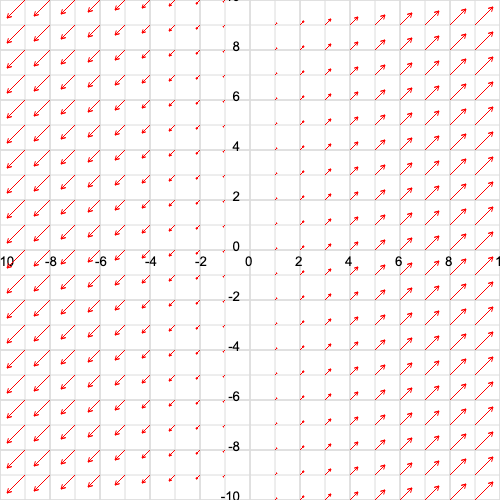
\includegraphics[width=\textwidth]{Figures/vec_v.png}
            \caption{Vector field $\mathbf{v}$.}
            \end{subfigure}
            ~
            \begin{subfigure}[h]{.45\textwidth}
            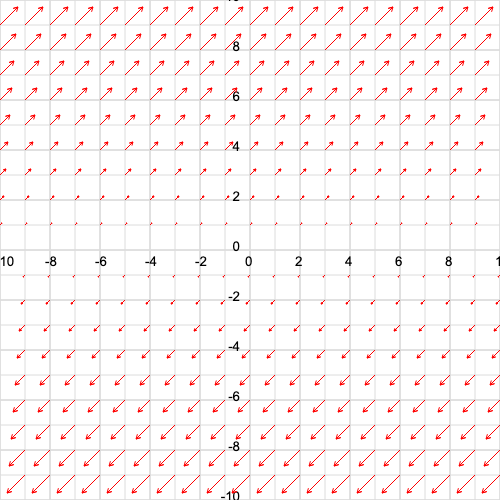
\includegraphics[width=\textwidth]{Figures/vec_u.png}
            \caption{Vector field $\mathbf{u}$.}
            \end{subfigure}
        \end{figure}
        Adding these results in the field
        \begin{figure}[H]
            \centering
            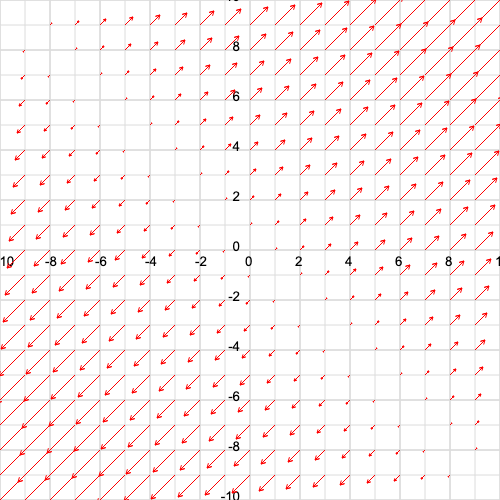
\includegraphics[width=.45\textwidth]{Figures/v_field_1.png}
            \caption{Caption}
            \label{fig:vec_field_1}
        \end{figure}
        \end{ex}
%        
        \begin{remark}
        If we do this all for vector fields, we can take curves and scalar fields as special cases.
        \begin{itemize}
            \item Adding together scalar fields is the same as adding functions.  They just have more inputs to think about!
            \item Adding together curves is done in the same componentwise manner that we have shown here for vector fields.
        \end{itemize}
        \end{remark}
        
        We can also scale a field by a real number.  This will stretch vectors at each point.
        
        \begin{ex}{Scaling of Vector Fields}{scale_vect_field}
        Just take the vector field
        \[
        \mathbf{v}(x,y,z)=(f_1(x,y,z),f_2(x,y,z),f_3(x,y,z))
        \]
        then we can take
        \[
        \lambda \mathbf{v}=(\lambda f_1, \lambda f_2, \lambda f_3).
        \]
        \end{ex}
        
        \begin{remark}
        There is many reasons why the above is important.  It seems our physical world plays nicely with the above concept, for one.
        
        One thing we can actually do, and will do a bit later, is find that there are two main types of vector fields in $\R^3$.  These will be the curl fields and divergence fields!  This is important in electromagnetism.
        \end{remark}
        
        When we were working with complex numbers, we considered integrating a complex function $f(z)$ over a contour $\gamma(t)$ from $t=a$ to $t=b$.  This involved computing
        \[
        \int_\gamma f(\gamma)d\gamma = \int_a^b f(\gamma(t))\gamma'(t)dt.
        \]
        I introduced this concept since it appears in the context of multivariate functions.  However, in the multivariate case, we needed some more tools.
        
        Now, the idea is as follows.  We will be given a scalar field, $f(x,y,z)$ or a vector field $\mathbf{F}(x,y,z)$ and a curve $\gamma(t)$.  
        
        \section{Line integrals of scalar fields}
        For the purpose of visualization, we will look at scalar fields of two variables and curves in the plane.  Our set up will have $f(x,y)$ and $\gamma(t)$ over the time $t=a$ to $t=b$.
        
        We want to understand the following:
        \[
        \int_\gamma f(\gamma)d\gamma \coloneqq \int_a^b f(\gamma(t))\|\gamma'(t)\|dt.
        \]
        Intuitively speaking, this integral finds the area under the curve $\gamma$ along the graph of $f$.  This is analogous to what we did in one dimension! See the following figure.
        \begin{figure}[H]
            \centering
            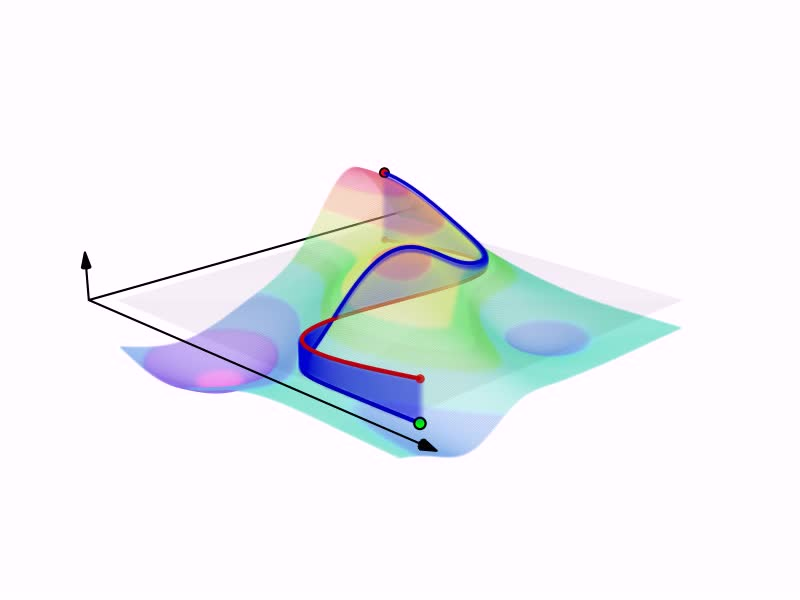
\includegraphics[width=.5\textwidth]{Figures/Line_integral_of_scalar_field.jpg}
        \end{figure}
        
        \begin{ex}{Length of a curve}{length_of_curve}
        Let $f(x,y,z)=1$ and $\gamma(t)$ be a curve over $t=a$ to $t=b$.  Then the line integral
        \[
        \int_\gamma f(\gamma)d\gamma = \int_a^b \|\gamma'(t)\|dt
        \]
        is known as the \emph{length} (sometimes \emph{arclength} of the curve $\gamma$.
        \end{ex}
        
        \begin{ex}{Line Integral on a Paraboloid}{line_int_parabooid}
        Consider the function $f(x,y)=x^2+y^2$ and $\gamma(t)=(t,t)$ over $t=0$ to $t=1$.  Then the line integral
        \[
        \int_\gamma f(\gamma)d\gamma = \int_0^1 f(\gamma(t))\|\gamma'(t)\|dt.
        \]
        We have
        \begin{itemize}
            \item $f(\gamma(t))=t^2+t^2=2t^2.$
            \item $\|\gamma'(t)\|=\|(1,1)\|=\sqrt{2}.$
        \end{itemize}
        So we have
        \[
        \int_\gamma f(\gamma)d\gamma = \int_0^1 2\sqrt{2}t^2dt.
        \]
        This evaluates to $\frac{2\sqrt{2}}{3}$.
        \end{ex}
        
        \begin{exercise}
        Integrate $f(x,y)=x+y$ along the curve $\gamma(t)=(t,0)$ from $t=0$ to $t=1$. What do you notice about this? Can we tie this to one-dimensional integration?
        \end{exercise}
        
        \section{Line integrals of vector fields}
        
        There is also a type of line integral that works alongside vector fields.  Roughly, the idea is to add up how much a vector field is pointing along the curve throughout the length of the curve.  
        
        Here we are given $\mathbf{F}(x,y,z)$ is a vector field, $\gamma(t)$ is a curve over the time $t=a$ to $t=b$.  Then we can write
        \[
        \int_\gamma \mathbf{F}(\gamma)\cdot d\gamma =\int_a^b \mathbf{F}(\gamma(t))\cdot \gamma'(t) dt.
        \]
        
        \begin{ex}{Work Done on a Particle}{work_on_particle}
        The work done on a particle (or change in energy) is written as a line integral of this form.  
        
        Take for example, $\mathbf{F}(x,y)=(2x,3y)$ and $\gamma(t)=(t,t^2)$ over the time $t=0$ to $t=1$.  Then
        \begin{align*}
        \int_\gamma \mathbf{F}(\gamma)\cdot d\gamma &= \int_0^1 \mathbf{F}(t,t^2)\cdot (t,t^2)dt\\
        &= \int_0^1 (2t,2t^2)\cdot(t,t^2)dt\\
        &=\int_0^1 2t^2+2t^4dt.
        \end{align*}
        Which I'll leave to you to evaluate if you'd like.
        \end{ex}
        
        \begin{remark}
        This notion is extremely important in defining something called the \emph{potential} of a vector field.  This will show up in electrodynamics.
        
        If the force in the example above is \emph{conservative}, we will have a potential.  This will correspond nicely to the vector field having no \emph{curl}.
        \end{remark}
        
        \section{Derivatives}
        Having done some integral calculus, it's time to head back to differential calculus.  We should say the following. This is far more abstract than we need, but it is an important realization.  
        
        \begin{df}{The Derivative}{derivative}
        Given a function $f\colon \R^n \to \R^m$, the \textbf{derivative of $f$ at the point $\mathbf{x}_0$} is the best \emph{linear approximation} to $f$ at the point $\mathbf{x}_0$.
        
        What this means is the following: If we zoom in to the point $\mathbf{x}_0$ and see what $f$ does in this region, we'll notice that $f$ is approximately a linear transformation.
        \end{df}
        
        Now, let us review the one-dimensional derivative that we are familiar with.
        
        \begin{df}{Derivative on $\R$}{der_on_R}
        Given $f\colon \R \to \R$, we define the \textbf{derivative $f'$ of $f$ at the point $x_0$} by
        \[
        f'(x_0)\coloneqq \lim_{\delta \to 0} \frac{f(x_0+\delta)-f(x_0)}{\delta}.
        \]
        This value $f'(x_0)$ is a number, and moreover is a $1\times 1$-matrix!  We often hide this idea at first.
        \end{df}
        
        It's a bit silly to say $f'(x_0)$ is a $1\times 1$-matrix, but in the end it will help us to remember this.
        
        \subsubsection{Derivatives of scalar fields}
        We can investigate functions of multiple variables in more ways than the single variable case.  Let us start with scalar fields.
        
        \begin{df}{Partial Derivatives}{partial_derivs}
        Let $f\colon \R^3 \to \R$ be a scalar field.  Then we can consider derivatives with respect to changing each input.  For example, we define the \textbf{partial derivative with respect to $x$} \textbf{at the point $(x_0,y_0,z_0)$}, denoted $\frac{\partial f}{\partial x}$, and put
        \[
        \frac{\partial f}{\partial x}(x_0,y_0,z_0)\coloneqq \lim_{\delta \to 0} \frac{f(x_0+\delta,y_0,z_0)-f(x_0,y_0,z_0)}{\delta}
        \]
        \end{df}
        
        \begin{remark}
        For partial derivatives, all but one variable are being held constant.  So, when you are computing these, be sure to treat the proper variables as constant when necessary.
        \end{remark}
        
        \begin{exercise}
        Define $\frac{\partial f}{\partial y}$ and $\frac{\partial f}{\partial z}$ in a similar way to the above definition.
        \end{exercise}
        
        \begin{exercise}
        Compute $\partialx$, $\partialy$, and $\partialz$ for the function 
        \[
        f(x,y,z)=\sin(xyz)+x+2y^2+3x^2z.
        \]
        \end{exercise}
        
        It turns out that collecting the partial derivatives as a vector is the best linear approximation to a scalar function.  We call this vector the gradient vector.
        
        \begin{df}{The Gradient}{gradient}
        Given a scalar field $f(x,y,z)$, the \textbf{gradient of $f$ at the point $(x_0,y_0,z_0)$}, denoted $\nabla f(x_0,y_0,z_0)$ is given by
        \[
        \nabla f(x_0,y_0,z_0)=\begin{bmatrix} \partialx(x_0,y_0,z_0)\\ \partialy(x_0,y_0,z_0)\\ \partialz(x_0,y_0,z_0)\end{bmatrix}.
        \]
        \end{df}
        
        \begin{exercise}
        Compute the gradient for the function
        \[
        f(x,y,z)=\sin(xyz)+x+2y^2+3x^2z.
        \]
        \end{exercise}
        
        \subsubsection{Properties of partial derivatives and the gradient}
        
        As with the one-dimensional derivative, we have some properties that will be helpful.\\
        
        \noindent\textbf{Partial Derivatives:}
        \begin{enumerate}[(i)]
            \item \textbf{Sum Rule:} Given $f(x,y,z)$ and $g(x,y,z)$, we have that
            \[
            \frac{\partial}{\partial x} (f(x,y,z)+g(x,y,z))=\partialx + \frac{\partial g}{\partial x}.
            \]
            Of course, this holds for any partial derivative.
            \item \textbf{Constant Multiple:} Given $\lambda \in \R$ and $f(x,y,z)$, we have that
            \[
            \frac{\partial}{\partial x}(\lambda f(x,y,z))=\lambda \partialx.
            \]
            Again, this holds for any partial derivative.
            \item \textbf{Product Rule:} Given $f(x,y,z)$ and $g(x,y,z)$ we have that
            \[
            \frac{\partial }{\partial x}(f(x,y,z)g(x,y,z))=\partialx g + f \frac{\partial g}{\partial x}.
            \]
            Ths holds for all partial derivatives.
        \end{enumerate}
        
        \begin{remark}
        The chain rule will show up eventually, but not yet.  As for the quotient rule, this also holds, but I don't show it here.
        \end{remark}
        
        \noindent\textbf{The Gradient:}
        \begin{enumerate}[(i)]
            \item \textbf{Sum Rule:} Given $f(x,y,z)$ and $g(x,y,z)$, we have that
            \[
            \nabla(f(x,y,z)+g(x,y,z))=\nabla f(x,y,z)+\nabla g(x,y,z).
            \]
            \item \textbf{Constant Multiple:} Given $\lambda \in \R$ and $f(x,y,z)$, we have that
            \[
            \nabla(\lambda f(x,y,z))=\lambda \nabla f(x,y,z).
            \]
            \item \textbf{Product Rule:} Given $f(x,y,z)$ and $g(x,y,z)$ we have that
            \[
            \nabla(f(x,y,z)g(x,y,z))=(\nabla f(x,y,z))g(x,y,z)+f(x,y,z)(\nabla g(x,y,z))
            \]
            
        \end{enumerate}
        
        We've learned how to compute partial derivatives and the gradient, but what are they really telling us? Remember that the derivative $\frac{d}{dx}$ of a function $f(x)$ tells us the rate of change of $f$ as we move in the $x$-direction.  This is very similar to what $\frac{\partial}{\partial x}$ tells us about a function $f(x,y,z)$.  So we can say the following.
        \begin{itemize}
            \item $\frac{\partial f}{\partial x}$ tells us how $f$ changes as we move in the $x$-direction.
            \item $\frac{\partial f}{\partial y}$ tells us how $f$ changes as we move in the $y$-direction.
            \item $\frac{\partial f}{\partial z}$ tells us how $f$ changes as we move in the $z$-direction.
        \end{itemize}
        
        We can put these together into the gradient $\nabla f$ and know how $f$ changes in each possible direction. Let's see how the gradient acts then. 
        
        \begin{ex}{Gradients on the Paraboloid}
        Let us start with $f(x,y)=x^2+y^2$.  Then
        \[
        \nabla f(x,y) = (2x,2y).
        \]
        Let us plot the level curves of this surface.
        \begin{figure}[H]
            \centering
            \begin{subfigure}[h]{.45\textwidth}
            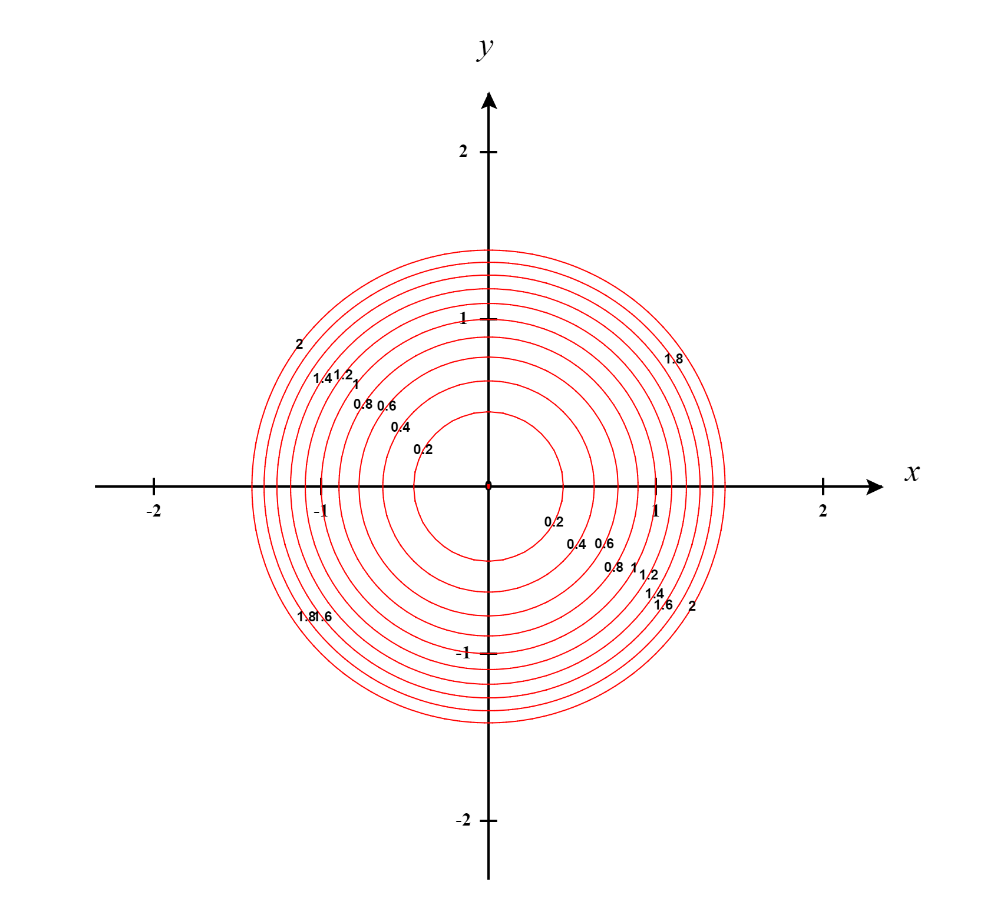
\includegraphics[width=\textwidth]{Figures/level_curves_gradient.png}
            \caption{Level curves of $f(x,y)$.}
            \end{subfigure}
            ~
            \begin{subfigure}[h]{.45\textwidth}
            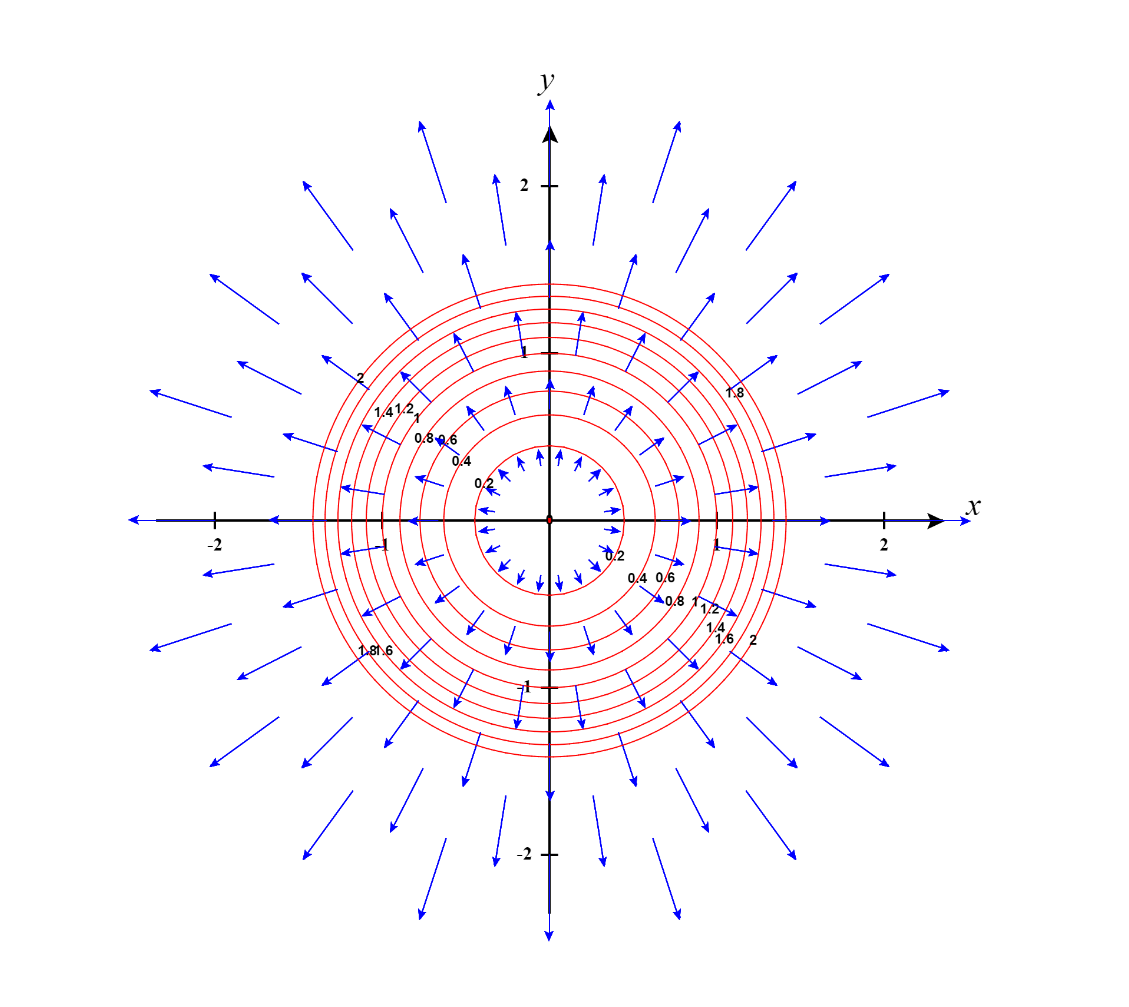
\includegraphics[width=\textwidth]{Figures/level_curves_gradient_vectors.png}
            \caption{Gradient vectors shown in blue.}
            \end{subfigure}
        \end{figure}
        \begin{itemize}
            \item Notice that the gradient vectors point in a direction perpendicular to the level curves and the length corresponds to how close the nearest level curve is.
            \item The gradient is zero at the bottom of this surface.  
        \end{itemize}
        \end{ex}
        
        \begin{prop}{Gradient Points Uphill}{gradient_prop}
        The gradient $\nabla f(x,y,z)$ is the vector that points in the direction of greatest increase for a function $f(x,y,z)$.
        \end{prop}
        
        How about second partial derivatives? What can we say here. We have each of the following for a function $f(x,y)$:
        \begin{itemize}
            \item $\frac{\partial^2 f}{\partial x^2}$
            \item $\frac{\partial^2 f}{\partial y^2}$
            \item $\frac{\partial}{\partial y}\frac{\partial f}{\partial x}$
            \item $\frac{\partial}{\partial x}\frac{\partial f}{\partial y}$
        \end{itemize}
        
        Recall what $\frac{d^2 f}{dx^2}$ meant for a function $f(x)$.  This told us how $f$ was curving (or what concavity $f$ had). The story is similar for these partial derivatives.
        
        \begin{itemize}
            \item $\frac{\partial^2 f}{\partial x^2}$ tells us about the concavity (or curvature) of $f$ as we move in the $x$ direction.
            \item $\frac{\partial^2 f}{\partial y^2}$ tells us about the concavity (or curvature) of $f$ as we move in the $y$ direction.
            \item We actually have that $\frac{\partial}{\partial y}\frac{\partial f}{\partial x}=\frac{\partial}{\partial x}\frac{\partial f}{\partial y}$.  This interpretation is a bit hard to deal with.  Let's not worry too much about it.
        \end{itemize}
        
        \begin{prop}{Partial Derivatives Commute}{partials_commute}
        We have that
        \[
        \frac{\partial}{\partial y}\frac{\partial f}{\partial x}=\frac{\partial}{\partial x}\frac{\partial f}{\partial y}.
        \]
        Moreover, for functions of more variables, we can say that the order we take derivatives does not matter.
        \end{prop}
        
        \begin{exercise}
        Given $f(x,y)=x^2+y^2$, compute
        \[
        \frac{\partial^2 f}{\partial x^2}, ~ \frac{\partial^2 f}{\partial y^2}, ~ \frac{\partial}{\partial y}\frac{\partial f}{\partial x},~ \frac{\partial}{\partial x}\frac{\partial f}{\partial y}.
        \]
        What can we say about the curvature of $f$ in the two directions? Does this make sense?
        \end{exercise}
        
        \section{Optimization}
        In single variable calculus, we optimized functions $f(x)$ by finding the point $x_0$ where 
        \[
        f'(x_0)=0.
        \]
        We called this a \emph{critical point}. We found if this optimizer $x_0$ was a maximizer or minimizer by checking the sign of second derivative $f''(x_0)$. We had
        \begin{align*}
            \textrm{Maximum: }& f''(x_0)<0\\
            \textrm{Minimum: }& f''(x_0)>0.
        \end{align*}
        
        In higher dimensions, this idea works similarly. We just have more to check. 
        
        \begin{df}{Stationary Points}{stationary_points}
        Given a function $f(x,y)$, we call a point $(x_0,y_0)$ a \textbf{stationary point} if 
        \[
        \nabla f(x_0,y_0) = \mathbf{0}.
        \]
        \end{df}
        
        As before, we will use second derivatives to find out whether this is a maximum or a minimum.
        
        \begin{prop}{Maximizers and Minimizers}{max_min}
        A stationary point $(x_0,y_0)$ is a 
        \begin{align*}
            \textrm{Maximizer if~ }& \frac{\partial^2 f}{\partial x^2} <0 \textrm{ ~and~ } \frac{\partial^2 f}{\partial y^2}<0,\\
            \textrm{Minimizer if~ }& \frac{\partial^2 f}{\partial x^2} >0 \textrm{ ~and~ } \frac{\partial^2 f}{\partial y^2}>0,\\
            \textrm{Saddle if otherwise.}
        \end{align*}
        \end{prop}
        
        \begin{exercise}
        Let
        \[
        f(x,y) = \frac{xy}{e^{x^2+y^2}}.
        \]
        \begin{enumerate}[(a)]
            \item Find all stationary points for $f$.
            \item Determine whether these points are minimizers or maximizers.
        \end{enumerate}
        \end{exercise}
        
        \begin{exercise}
        Show that $f(x,y)=xy$ has a saddle point at $(0,0)$.
        \end{exercise}
        
        \subsubsection{Lagrange Multipliers}
        Often times we are given a situation that we wish to find an optimum solution to, but we are somehow constrained.  A biological example would be fixing a given volume for a red blood cell, and finding the optimum shape so that oxygen diffusion is maximized.  A physical example would be finding the fastest path between two points when moving through a medium with varying viscosity.
        
        The idea is relatively tame. We are given the function to optimize
        \[
        f(x,y,z)
        \]
        and the constraining function
        \[
        g(x,y,z)=k.
        \]
        Then we must solve the equation
        \[
        \nabla f(x,y,z) = \lambda \nabla g (x,y,z)
        \]
        where $\lambda$ is called the \textbf{Lagrange multiplier}. Let's work through an example of solving this.
        
        \begin{ex}{Largest Box}{largest_box}
        Let's find the dimensions of the box with the largest volume if the total surface area is $64 cm^2$.  We must determine our function to optimize, which is the volume function
        \[
        V(x,y,z) = xyz.
        \]
        Our constraint is the surface area function $A(x,y,z)$ must be
        \[
        g(x,y,z)=2xy+2xz+2yz=64,
        \]
        which we will simplify as
        \[
        xy+xz+yz = 32.
        \]
        \begin{enumerate}
            \item We first take
            \[
            \nabla f(x,y,z) = \begin{bmatrix} yz \\ xz \\ xy \end{bmatrix}
            \]
            and
            \[
            \nabla g(x,y,z) = \begin{bmatrix} 2y+2z \\ 2x+2z \\ 2x+2y\end{bmatrix}.
            \]
            \item This gives us four equations to solve. Three are from the equation $\nabla f(x,y,z) =\nabla g(x,y,z)$
            \begin{align}
                yz &= \lambda (y+z)\\
                xz &= \lambda (x+z)\\
                xy &= \lambda (x+y),
            \end{align}
            and one is from the constraint $g(x,y,z)=64$
            \[
            xy+xz+yz = 32.
            \]
            \item Working through solving these can be nontrivial.  In this case, we can do the following: Multiply (1) by $x$, (2) by $y$, and $(3)$ by $z$.  Which gives us
            \begin{align*}
                xyz &= \lambda x(y+z)\\
                xyz &= \lambda y(x+z)\\
                xyz &= \lambda z(x+y)
            \end{align*}
            Now we can set the first two equal to find
            \[
            \lambda x(y+z)=\lambda y(x+z)
            \]
            which simplifies to 
            \[
            \lambda (xz-yz)=0
            \]
            meaning that $\lambda =0$ or $xz=yz$. Note that $\lambda =0$ is not possible since that will end up giving us zero surface area and we won't satisfy the constraint.
            
            Now $xz-yz=0$ means that $x=y$, which we can substitute back into the equations later. 
            
            We can set the last two equal to find
            \[
            \lambda y (x+z)=\lambda z(x+y)
            \]
            which with similar work tells us $z=y$.  So now we make note of $x=y$ and we have $x=y=z$.  
            
            So now we use the constraint equation with $x=y=z$ and find that we have
            \[
            x^2+y^2+z^2 = 3x^2 = 32
            \]
            which means that $x\approx 3.266$.  Thus
            \[
            V(3.266,3.266,3.266)\approx 34.8376
            \]
            is the largest volume.  \emph{This means our ideal solution is a cube!} 
            
        \end{enumerate}
        \end{ex}
        
        \section{Approximation and the Tangent Space}
        Sometimes it is helpful to know what a surface looks like up close.  In this case, the surface is best approximated by a plane.  This is analogous to how you can approximate functions of a single variable by a line.
        
        \begin{exercise}
        Compute the tangent line to $f(x)=2x^2+5$ at the point $x_0=3$.
        \end{exercise}
        
        \subsubsection{Equation for a Plane}
        
        We haven't worked much with planes in space yet, but we have seen surfaces.  In some sense, planes are the easiest surfaces.  They are, after all, linear objects.
        
        \begin{ex}{Plane and Normal}{plane_normal}
        The equation for a plane is given by
        \[
        ax+by+cz+ d = 0.
        \]
        Notice that this is a linear equation.
        
        Then the \emph{normal vector} to the plane is given by 
        \[
        \mathbf{n} = \begin{bmatrix} a \\ b \\ c\end{bmatrix}.
        \]
        We can see a diagram of this here.
        \begin{figure}[H]
            \centering
            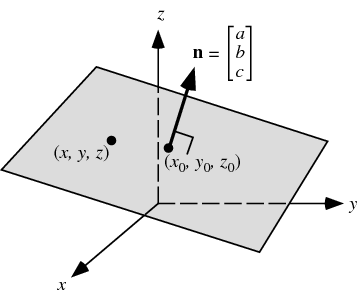
\includegraphics[width=.4\textwidth]{Figures/plane_n.png}
        \end{figure}
        \end{ex}
        
        Now, if we are given a surface (defined as a level surface or as the graph of a function), we can compute an approximation at a point called the \emph{tangent plane}.
        
        \begin{ex}{Tangent Plane to Paraboloid}
        Consider the function 
        \[
        f(x,y)=-x^2-y^2.
        \]
        Then the graph of the function is given by plotting the points
        \[
        (x,y,f(x,y)).
        \]
        We compute the tangent plane by computing partial derivatives. We take
        \begin{align*}
        \frac{\partial f}{\partial x} &= -2x\\    
        \frac{\partial f}{\partial y} &= -2y.
        \end{align*}
        Then the equation for a tangent plane at the point $(x_0,y_0,f(x_0,y_0))$ is given by
        \[
        z-f(x_0,y_0)=\partialx (x-x_0)+\partialy (y-y_0).
        \]
        So in our case, we have
        \[
        z-(-x_0^2-y_0^2)=-2x_0(x-x_0)-2y_0(y-y_0).
        \]
        Pictorially, it looks as follows (letting $p=(x_0,y_0,f(x_0,y_0))$):
        \begin{figure}[H]
            \centering
            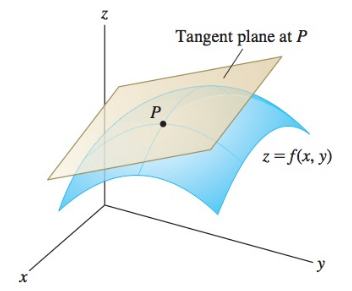
\includegraphics[width=.4\textwidth]{Figures/tangent-planes-1.png}
        \end{figure}
                
        \end{ex}
        
        \begin{ex}{Tangent Vectors}{tangent_vectors}
        Another way to understand this is to compute the \emph{tangent vectors} at a point. Take the same function $f(x,y)=-x^2-y^2$ and compute
        \begin{align*}
            \frac{\partial}{\partial x}\begin{bmatrix} x \\ y \\ f(x,y)\end{bmatrix} &= \begin{bmatrix} 1\\ 0 \\ -2x\end{bmatrix}\\
            \frac{\partial}{\partial y}\begin{bmatrix} x \\ y \\ f(x,y)\end{bmatrix} &= \begin{bmatrix} 0\\ 1 \\ -2y\end{bmatrix}.
        \end{align*}
        Then take the cross product of these two vectors to get the normal vector to the tangent plane
        \[
        \begin{bmatrix} 1 \\ 0 \\-2x\end{bmatrix} \times \begin{bmatrix} 0 \\ 1 \\ -2y\end{bmatrix} = \begin{bmatrix} 2x \\ 2y \\ 1\end{bmatrix}.
        \]
        Pick a point $(x_0,y_0)$ and the normal to tangent plane is given by
        \[
        \mathbf{n}=\begin{bmatrix} 2x_0 \\ 2y_0 \\ 1 \end{bmatrix}.
        \]
        Which leads us to the following equation of a plane (but not exactly the tangent plane)
        \[
        2x_0 x + 2y_0y+z=0.
        \]
        This plane is parallel to the tangent plane and is often a nicer tool.
        \end{ex}
        
        \begin{exercise}
        Take the two equations for the planes above and simplify each to having a zero right hand side.  Then subtract each of these equations from each other and see what the difference is.
        \end{exercise}
        
        
    \chapter{Calculus with Vector Fields}
        \section{The Jacobian of a Vector Field}
        Recall we can define a three dimensional vector field $\mathbf{v}(x,y,z)$ by
        \[
        \mathbf{v}(x,y,z)=(v_1(x,y,z),v_2(x,y,z),v_3(x,y,z)) = \begin{bmatrix} v_1(x,y,z) \\ v_2(x,y,z) \\ v_3(x,y,z) \end{bmatrix}
        \]
        where we call each $v_1$, $v_2$, and $v_3$ the component functions.  Notice that each component function is a scalar function!
        
        Since each component function is a scalar function, we know how to compute the derivative of each by computing the gradient.  This gives us a way to then talk about the derivative of the vector field as a whole
        
        \begin{df}{Jacobian}{jacobian}
        The \textbf{Jacobian} of a vector field $\mathbf{v}(x,y,z)$ is a matrix
        \[
        J(x,y,z)\coloneqq \begin{bmatrix} \nabla v_1^T \\ \nabla v_2^T \\ \nabla v_3^T \end{bmatrix},
        \]
        where the gradients are transposed (the superscript $T$) so they are are written as row vectors and placed in a matrix. More specifically, we can write this matrix as 
        \[
        J(x,y,z) = \begin{bmatrix} \frac{\partial v_1}{\partial x} & \frac{\partial v_1}{\partial y} & \frac{\partial v_1}{\partial z}\\ \frac{\partial v_2}{\partial x} & \frac{\partial v_2}{\partial y} & \frac{\partial v_2}{\partial z} \\ \frac{\partial v_3}{\partial x} & \frac{\partial v_3}{\partial y} & \frac{\partial v_3}{\partial z} \end{bmatrix}.
        \]
        \end{df}
        
        The Jacobian contains a lot of information. Intuitively, it tells us how each component of the vector field changes in each direction.  
        
        \begin{ex}{Computing the Jacobian, 1}{computing_jacobian}
        Let us consider the vector field
        \[
        \mathbf{v}(x,y,z) = (x^2+y^2,z,x+y+z).
        \]
        Then we can write
        \begin{align*}
            v_1(x,y,z)&= x^2+y^2\\
            v_2(x,y,z)&= z\\
            v_3(x,y,z)&= x+y+z.
        \end{align*}
        So we compute the gradients of each
        \begin{align*}
            \nabla v_1 &= \begin{bmatrix} 2x \\ 2y \\ 0 \end{bmatrix}\\
            \nabla v_2 &= \begin{bmatrix} 0 \\ 0 \\ 1 \end{bmatrix}\\
            \nabla v_3 &= \begin{bmatrix} 1 \\ 1 \\ 1 \end{bmatrix}.
        \end{align*}
        So then the Jacobian is
        \[as
        J(x,y,z) = \begin{bmatrix} 2x & 2y & 0 \\ 0 & 0 & 1\\ 1 & 1 & 1 \end{bmatrix}.
        \]
        \end{ex}
        
        A related and important quantity comes in the form of the determinant of the Jacobian.  We've previously talked about the determinant of a matrix as telling us the (signed) scaling of volume of a linear transformation.  That is, for example, if we have
        \[
        A = \begin{bmatrix} 2 & 0 & 0\\ 0 & 2 & 0\\ 0 & 0 & 2 \end{bmatrix}
        \]
        then $\det(A)=8$ and we say that volumes of parallelopipeds are increased by a factor of $8$ in this case.  
        
        When you are given a vector field, you can think of different regions of space being stretched differently.  This is why we have that the Jacobian is a matrix that depends on the position $(x,y,z)$.  In this case, the volumes that are being stretched are very very tiny parallelopipeds.  You can think of cubes with side lengths $dx$, $dy$, and $dz$. 
        
        \begin{ex}{Computing the Jacobian, 2}
        We found that given
        \[
        \mathbf{v}(x,y,z) = (x^2+y^2,z,x+y+z)
        \]
        that
        \[
        J(x,y,z) = \begin{bmatrix} 2x & 2y & 0 \\ 0 & 0 & 1 \\ 1 & 1 & 1 \end{bmatrix}
        \]
        As we can see, this matrix depends on position.  Let's compute the determinant
        \[
        |J(x,y,z)|=\det(J(x,y,z))=2(y-x). 
        \]
        Something weird seems to happen with $y=x$ as the determinant $|J(x,y,z)|$ will be zero in this case. Otherwise, things are fine.
        \end{ex}
        
        \section{Divergence and Curl}
        Often we do not need to use the whole Jacobian.  We will find it to be necessary for integration, however.  
        
        For analysis of vector fields, we often wish to break them into their smaller pieces.  Fundamentally, we can break vector fields into two parts:
        \begin{itemize}
            \item Sources and sinks,
            \item Rotations.
        \end{itemize}
        
        \subsubsection{Sources, Sinks, and Divergence Fields}
        With some vector fields, we can make the analogy that some quantity (think air or water) is being added or removed from the system.  We call these \emph{sources} and \emph{sinks} respectively.  We want to quantify how much of some quantity is being added. This quantity is called the \emph{divergence}.
        
        Recall, we can write
        \[
        \nabla = \begin{bmatrix} \frac{\partial}{\partial x} \\ \frac{\partial}{\partial y} \\ \frac{\partial}{\partial z} \end{bmatrix}.
        \]
        If we are also given a vector field
        \[
        \mathbf{v}(x,y,z) = \begin{bmatrix} v_1(x,y,z) \\ v_2(x,y,z) \\ v_3(x,y,z) \end{bmatrix},
        \]
        we can compute the \textbf{divergence} of $\mathbf{v}$ by
        \[
        \nabla \cdot \mathbf{v}(x,y,z) = \frac{\partial v_1}{\partial x} + \frac{\partial v_2}{\partial y} + \frac{\partial v_3}{\partial z}.
        \]
        Notice that this quantity is a scalar!  This scalar value, the divergence, tells us how much the vector field is diverging at a point $(x,y,z)$. In other words, it tells us how much of a quanitity is being added or removed there.
        
        \begin{ex}{Source Field}{source_field}
        Consider
        \[
        \mathbf{v}(x,y,z) = \begin{bmatrix} x \\ y \\ z \end{bmatrix}.
        \]
        Then the divergence is
        \[
        \nabla \cdot \mathbf{v}(x,y,z) = \frac{\partial v_1}{\partial x} + \frac{\partial v_2}{\partial y} + \frac{\partial v_3}{\partial z} = 1 + 1 + 1 = 3.
        \]
        We can think of a source of air being placed at each point that pumps in $3$ units of air per second, or specifically being pumped in at the origin. The vector field looks like:
        \begin{figure}[H]
            \centering
            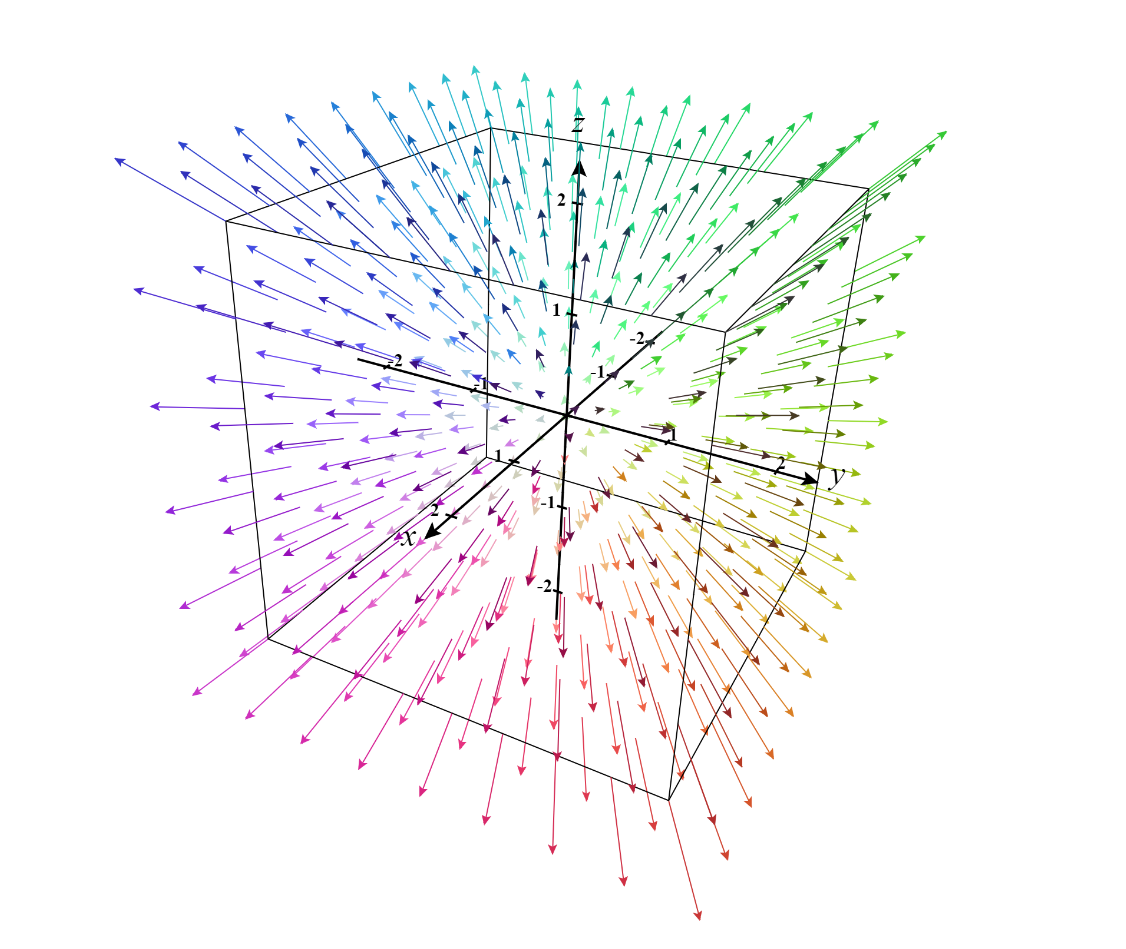
\includegraphics[width=.6\textwidth]{Figures/divergence_field.png}
        \end{figure}
        \end{ex}
        
        \subsubsection{Rotation Fields}
        The divergence was the quantity that measured the outflow from a point for a vector field.  The other quantity we can measure is the rotation of a vector field at a point.
        
        We define the \textbf{curl} of a vector field $\mathbf{v}(x,y,z)$ to be
        \[
        \nabla \times \mathbf{v}(x,y,z) = \begin{bmatrix} \frac{\partial v_3}{\partial y} - \frac{\partial v_2}{\partial z} \\ \frac{\partial v_1}{\partial z} - \frac{\partial v_3}{\partial x} \\ \frac{\partial v_2}{\partial x} - \frac{\partial v_1}{\partial y} \end{bmatrix}.
        \]
        \emph{Note that the curl is a vector!} The curl is a vector that points orthogonally to the plane where rotation occurs and has magnitude relative to how quickly the field swirls.
        
        It's a bit involved to go through the work and see exactly why this is the correct quantity for seeing rotation of a vector field.  However, you can recall that the cross product was useful in describing rotational motion of rigid bodies (that is, it showed up in angular velocity/momentum).
        
        \begin{ex}{A Rotation Field}{rot_field}
        Consider the vector field
        \[
        \mathbf{v}(x,y,z) = (-y,x,z)
        \]
        which looks like
        \begin{figure}[H]
            \centering
            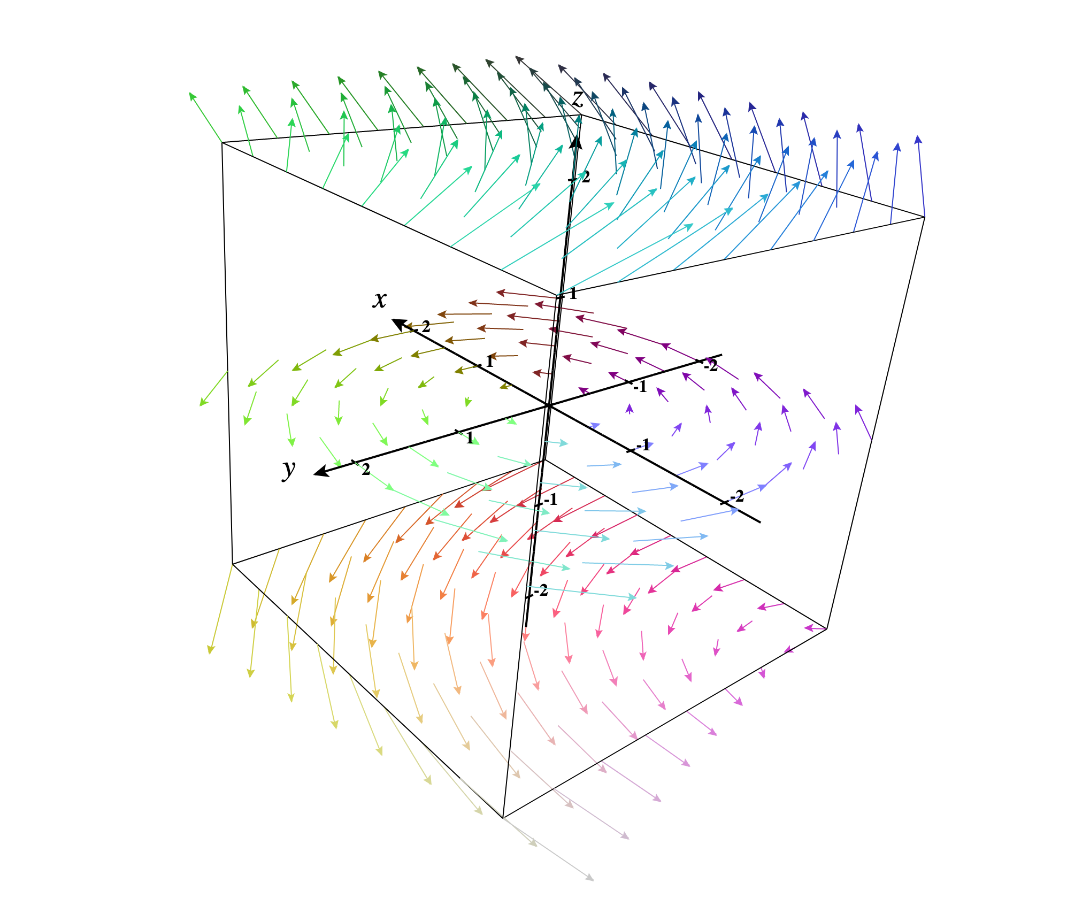
\includegraphics[width=.6\textwidth]{Figures/curl_field.png}
        \end{figure}
        We let
        \begin{align*}
            v_1(x,y,z) &= -y\\
            v_2(x,y,z) &= x\\
            v_3(x,y,z) &= z.
        \end{align*}
        If we look in this figure where $z=0$, we can clearly see that this field swirls around the origin.  If the curl is to measure rotation, we should see it nonzero here.
        
        Let us compute the curl of this field.  For this, we will all the other partial derivatives not contained in the divergence. That is, we need
        \begin{align*}
            \frac{\partial v_1}{\partial y} &= -1 & \frac{\partial v_1}{\partial z} &= 0\\
            \frac{\partial v_2}{\partial x} &= 1& \frac{\partial v_2}{\partial z} &= 0\\
            \frac{\partial v_3}{\partial x} &= 0 &  \frac{\partial v_3}{\partial y} &=0.
        \end{align*}
        Then we have
        \[
        \nabla \times \mathbf{v}(x,y,z) = \begin{bmatrix} 0-0\\ 0-0 \\ 1-(-1)\end{bmatrix} = \begin{bmatrix} 0\\ 0 \\ 2\end{bmatrix}.
        \]
        
        We can decipher the meaning here by saying that the swirling occurs in planes parallel to the $xy$-plane since the direction of the curl is only in the $z$-direction.  That is, curl is pointing perpendicularly to the plane of rotation.  How quickly the field swirls is given by the magnitude of the curl which is $2$ in this case.  Using the right hand rule we discussed previously this tells us the direction of swirling as well.  We have swirling counter-clockwise in the planes parallel to the $xy$-plane, and so we expect the curl to point in the positive $z$-direction.
        
        Take a moment to analyze this using the figure provided or by plotting this yourself.
        \end{ex}
        
        \begin{ex}{Divergence of the Rotation Field}
        One may also consider the divergent nature of the field 
        \[
        \mathbf{v}(x,y,z) = (-y,x,z)
        \]
        from the previous example and find that 
        \[
        \nabla \cdot \mathbf{v}(x,y,z) = 1.
        \]
        So, there is in some way divergence as well.  This leads us to breaking the vector field into a part that swirls and a part that diverges as follows:
        \begin{align*}
            \mathbf{v}_\textrm{swirl}(x,y,z) &= (-y,x,0)\\
            \mathbf{v}_\textrm{div}(x,y,z) &= (0,0,z).
        \end{align*}
        This type of analysis can be very helpful when considering real world problems.  It is especially important in electromagnetism.
        \end{ex}
        
        \subsubsection{Constant Vector Fields}
        Most of the understanding of vector fields was just covered by understanding the the part that diverges and the part that curls.  However, you can always add constants to these vector fields and these constants will not change the divergence or curl. Why? Take the following example.
        
        \begin{ex}{Constant Fields}{const_field}
        Let 
        \[
        \mathbf{v}(x,y,z) = (c_1,c_2,c_3)
        \]
        where $c_1,c_2,$ and $c_3$ are constants.  Then we can compute the Jacobian of $\mathbf{v}$
        \[
        J(x,y,z) = \begin{bmatrix} 0 & 0 & 0 \\ 0 & 0 & 0\\ 0 & 0 &0 \end{bmatrix}.
        \]
        Since the Jacobian holds all the partial derivative information, we can know from this that 
        \begin{align*}
            \nabla \cdot \mathbf{v} &= 0\\
            \nabla \times \mathbf{v} &= \mathbf{0}.
        \end{align*}
        \end{ex}
        
        \begin{exercise}
        Specifically show that the divergence and curl of a constant vector field (as in the previous example) are zero.  
        \end{exercise}
        
        All of this is to say that aside from the addition of a constant vector field, we understand the behavior by looking at divergence and curl.
        
        \section{The Laplacian of a Scalar Field}
        In the study of partial differential equations (PDEs), we are often asked to find a function $u(x,y,z)$ that satisfies the following equation
        \[
        \nabla \cdot \nabla u(x,y,z) = f(x,y,z)
        \]
        for some given function $f(x,y,z)$.  We will revisit this Part III, but for now we should see exactly what we mean by
        \[
        \nabla \cdot \nabla u(x,y,z).
        \]
        
        \begin{exercise}
        Show that
        \[
        \nabla \cdot \nabla u(x,y,z) = \frac{\partial^2 u}{\partial x^2} + \frac{\partial^2 u}{\partial y^2} + \frac{\partial^2 u}{\partial z^2}.
        \]
        \end{exercise}
        
        \begin{df}{Laplacian}{laplacian}
        We define the quantity
        \[
        \nabla \cdot \nabla u(x,y,z)
        \]
        to be the \textbf{Laplacian of $u(x,y,z)$} and we often write
        \[
        \Delta \coloneqq \nabla \cdot \nabla
        \]
        and call this the \textbf{Laplacian operator}.
        \end{df}
        
        Intuitively, the Laplacian can be summed up in a few ways. 
        \begin{itemize}
            \item The Laplacian is the \emph{divergence} of the \emph{gradient} of a scalar function.
            \item The Laplacian is the sum of ``curvatures" in each direction.
        \end{itemize}
        
        \begin{ex}{Computing the Laplacian}{compute_laplacian}
        Let us consider the functions
        \[
        f(x,y) = x^2+y^2
        \]
        and
        \[
        g(x,y) = x^2-y^2.
        \]
        Then we can compute the gradients of each function to get
        \begin{align*}
            \nabla f(x,y) &= \begin{bmatrix} 2x \\ 2y \end{bmatrix}\\
            \nabla g(x,y) &= \begin{bmatrix} 2x \\ -2y \end{bmatrix}.
        \end{align*}
        We can then compute the divergence of each of these and find
        \begin{align*}
            \nabla \cdot \nabla f(x,y) &= 2+2 = 4\\
            \nabla \cdot \nabla g(x,y) &= 2-2 =0.
        \end{align*}
        Let us see what these two functions look like to get a bit of an intuitive feel.
        \begin{figure}[H]
            \centering
            \begin{subfigure}[h]{.45\textwidth}
            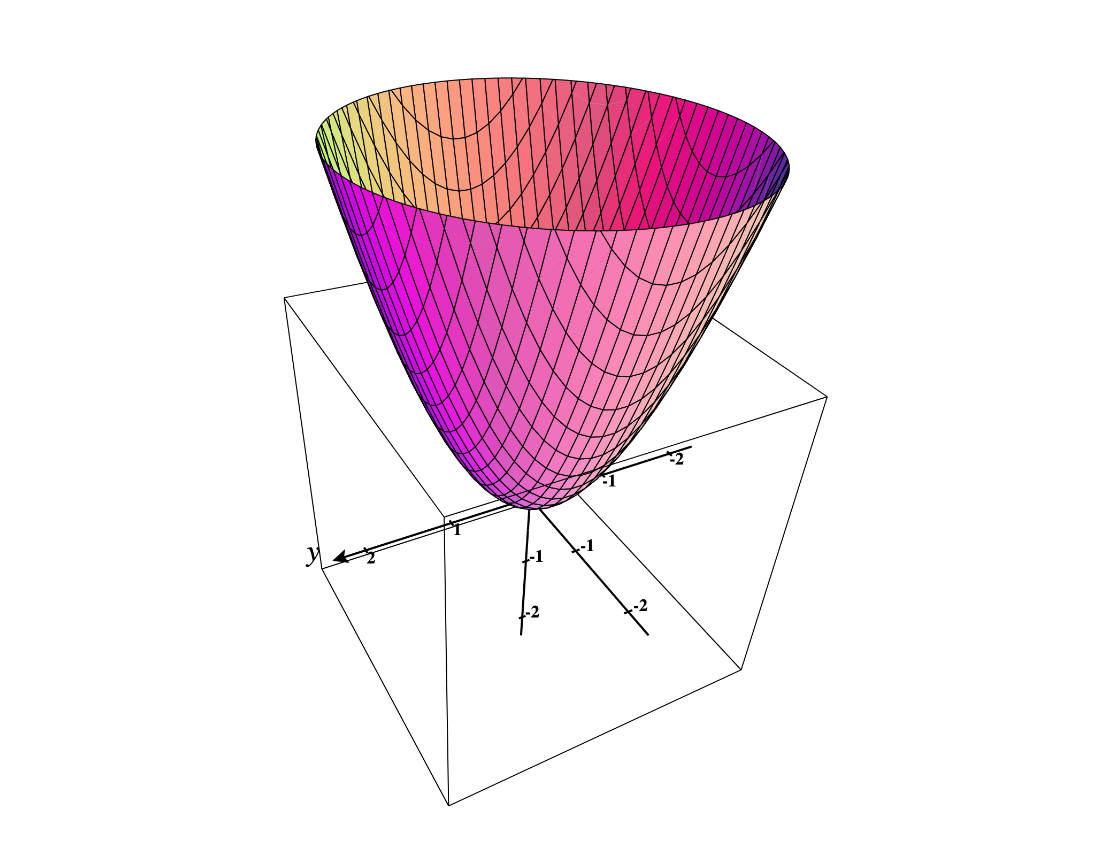
\includegraphics[width=\textwidth]{Figures/pos_laplace.png}
            \caption{A plot of $f(x,y).$}
            \end{subfigure}
            ~
            \begin{subfigure}[h]{.45\textwidth}
            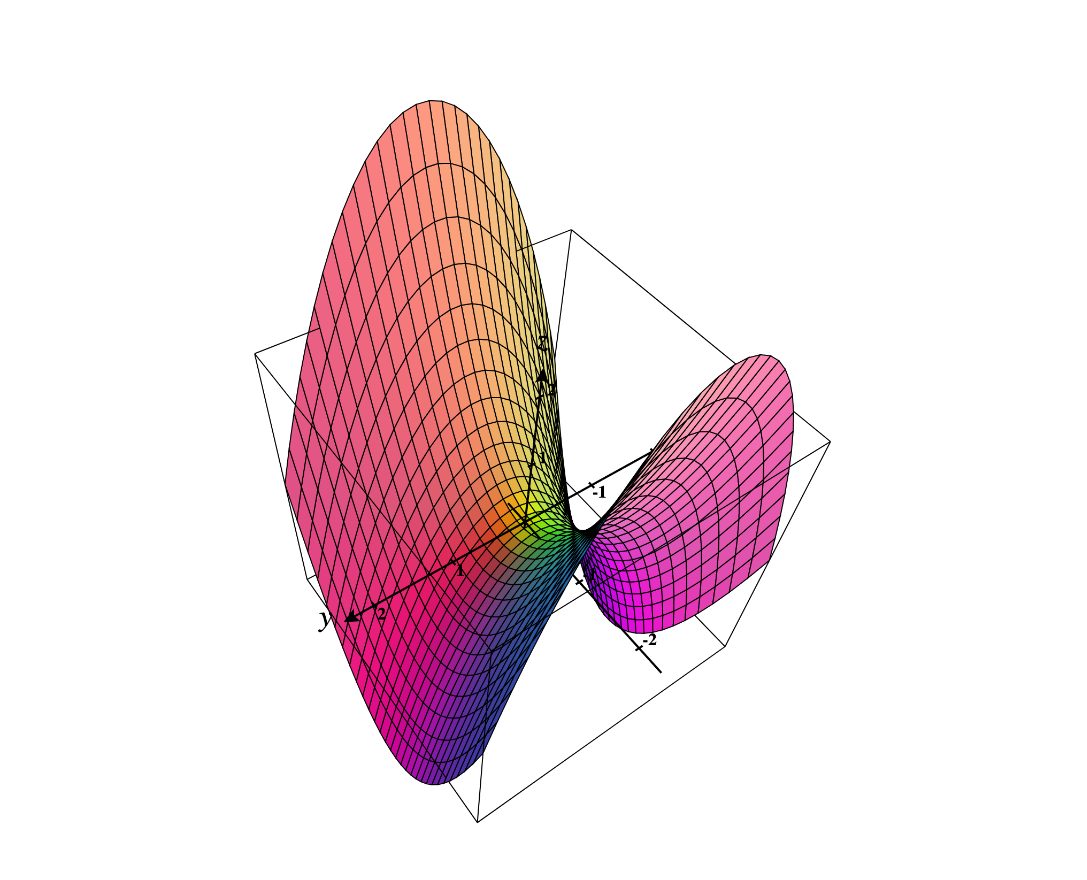
\includegraphics[width=\textwidth]{Figures/0_laplace.png}
            \caption{A plot of $g(x,y).$}
            \end{subfigure}
        \end{figure}
        Fundamentally we can see that these two functions are different.  It seems that for $f(x,y)$ we are curving upward in both the $x$ and $y$ direction which is what allows the Laplacian to be positive. However, for $g(x,y)$ one direction curves the opposite direction as the other which cancels out and gives us that the Laplacian is zero.  
        
        It turns out that the Laplacian describes many phenomenon. Two examples would be soap films and temperature flow.
        \end{ex}

        
        We have covered all of the differential calculus of multivariate functions that we need.  That does not mean it won't show up again, but the material won't be new.  We now move onto integration in multiple dimensions.
        
        \chapter{Integration in Multiple Dimensions}
        
        \section{Integration of Scalar Fields}
        
        \subsubsection{One Dimensional Case}
        In the case of one dimensional functions, we integrated to find the area under a curve.  That is, we were given a function $f(x)$ and asked to find
        \[
        \int_a^b f(x)dx
        \]
        which gave us the \emph{net} area under the curve.  Let's briefly review this with an example.
        
        \begin{ex}{One-Dimensional Integral}
        Let $f(x) = x^2+2$, $a=1,$ and $b=2$. Then we want to find
        \[
        \int_a^b f(x)dx = \int_1^2 x^2+2dx.
        \]
        Then we use the \emph{Fundamental Theorem of Calculus}. So, we find the antiderivative of the integrand and evaluate at the endpoints as follows
        \begin{align*}
            \int_1^2 x^2+2dx &= \left[ \frac{x^3}{3}+2x\right]_1^2\\
            &= \left(\frac{2^3}{3}+2(2)\right) - \left( \frac{1^3}{3}+2(1)\right)\\
            &= \frac{13}{3}.
        \end{align*}
        \end{ex}
        
        \subsubsection{Two Dimensional Case}
        
        Say we are now given a function $f(x,y)$ and bounds on both the $x$ and $y$ by
        $x_0 \leq x \leq x_1$ and $y_0 \leq y \leq y_1$.  We then wish to evaluate
        \[
        \int_{y_0}^{y_1} \int_{x_0}^{x_1} f(x,y)dxdy.
        \]
        You can think of this integral as being the \emph{net} volume under the surface given by $f(x,y)$.  
        
        How do we compute such an integral? The answer is iteratively.  Let's see how we do this with a concrete example.
        
        \begin{ex}{Two-Dimensional Integral}{2d_int}
        Let $f(x,y)=xy$, $x_0=1$, $x_1=2$, $y_0=3$ and $y_1=4$.  So, we want to evaluate
        \[
        \int_{y_0}^{y_1}\int_{x_0}^{x_1} f(x,y)dxdy = \int_3^4 \int_1^2 xy dxdy.
        \]
        The way we do this is by first evaluating the integral with respect to $x$ (holding $y$ constant) and then integrate with respect to $y$ ($x$ will not appear here). So, we integrate from the inside out.  
        
        Let's start by integrating with respect to $x$. We take
        \begin{align*}
            \int_1^2 xy dx &= \left[ \frac{x^2y}{2}\right]_1^2\\
            &= \left( y\frac{2^2}{2}\right) - \left(y\frac{1^2}{2}\right)\\
            &=\frac{3}{2}y.
        \end{align*}
        Now we take this function of $y$, and we integrate this with the bounds we are given.  
        \begin{align*}
            \int_3^4 \frac{3}{2}y dy &= \left[ \frac{3y^2}{4} \right]_3^4\\
            &= \frac{21}{4}.
        \end{align*}
        So we say that
        \[
        \int_3^4 \int_1^2 xy dxdy = \frac{21}{4}.
        \]
        
        Let's walk through the steps again. We did
        \begin{align*}
            \int_{y_0}^{y_1} \int_{x_0}^{x_1} f(x,y)dxdy&= \int_3^4\int_1^2 xy dxdy\\
            &= \int_3^4 \frac{3}{2}ydy \\
            &= \frac{21}{4}.
        \end{align*}
        \end{ex}
        
        \subsubsection{Three Dimensional Case}
        
        Integration here is performed in the same way.  We are given a function $f(x,y,z)$ and bounds on $x$, $y$, and $z$ such as $x_0\leq x \leq x_1$, $y_0\leq y\leq y_1$, and $z_0\leq z \leq z_1$. Then we evaluate
        \[
        \int_{z_0}^{z_1}\int_{y_0}^{y_1}\int_{x_0}^{x_1} f(x,y,z)dxdydz.
        \]
        Let's work through an example.
        
        \begin{ex}{Three-Dimensional Integral}{3d_int}
        Let
        \[
        f(x,y,z)=2x + 8xyz + 3,
        \]
        $x_0 = 0$, $x_1=1$, $y_0=2$, $y_1=3$, $z_0 =4$, $z_1=5$.  Then we want to find
        \[
        \int_{z_0}^{z_1}\int_{y_0}^{y_1}\int_{x_0}^{x_1} f(x,y,z)dxdydz = \int_4^5 \int_2^3 \int_0^1 2x+8xyz+3dxdydz.
        \]
        We do this iteratively.  So we first evaluate the $x$ integral holding the other variables constant for now.
        \begin{align*}
            \int_0^1 2x+8xyz+3 dx &= \left[ x^2 + 4x^2yz+3x\right]_0^1\\
            &= \left( 1^2 + 4(1)^2yz+3(1)\right) - \left( 0^2+4(0)^2yz+3(0)\right)\\
            &= 4yz+4.
        \end{align*}
        We then take this, and integrate with respect to $y$.
        \begin{align*}
            \int_2^3 4yz + 4 dy &= \left[ 2y^2z+4y\right]_2^3\\
            &= (4(3)^2z+4(3))-(4(2)^2z+4(2))\\
            &= 10z+4.
        \end{align*}
        Lastly, we integrate with respect to $z$
        \begin{align*}
            \int_4^5 10z+4 dz &= \left[ 5z^2+4z\right]_4^5\\
            &= (5(5)^2+4(5))-(5(4)^2+4(4))\\
            &=49.
        \end{align*}
        So we say that
        \[
        \int_4^5 \int_2^3 \int_0^1 2x+8xyz+3dxdydz = 49.
        \]
        Again, let's walk through the steps a bit
        \begin{align*}
            \int_{z_0}^{z_1}\int_{y_0}^{y_1}\int_{x_0}^{x_1} f(x,y,z)dxdydz &= \int_4^5 \int_2^3 \int_0^1 2x+8xyz+3dxdydz\\
            &= \int_4^5 \int_3^4 4yz+4dydz\\
            &= \int_4^5 10z+4dz\\
            &= 49.
        \end{align*}
        \end{ex}
        
        \section{Antiderivatives}
        In one variable calculus, we found that there is a relationship between the derivative and the indefinite integral.  In fact, this led us to call the indefinite integral the antiderivative.  This relationship was that
        \[
        \frac{d}{dx}\int f(x)dx = f(x)
        \]
        and
        \[
        \int \frac{df}{dx} = f(x) + C.
        \]
        From this, we realized that the indefinite integral is almost an inverse operation of the derivative.  It's just that in the case where we integrate a derivative, we only determine the function up to an additive constant. 
        
        \subsubsection{Potential Functions}
        The higher dimensional analog happens to be a bit more nuanced but the idea remains the same. Let's say we are given a function $f(x,y,z)$ and we compute, for example,
        \[
        \partialx.
        \]
        The issue now becomes this.  Let's say that we let
        \[
        f(x,y,z) = x+yz.
        \]
        Then we have that
        \[
        \partialx = 1.
        \]
        The terms with just a $y,z$ dependence disappear.  So if we were to try to undo this with an integral, we find that 
        \[
        \int \partialx dx = \int 1 dx = x + g(y,z).
        \]
        That is to say, when we take an indefinite integral a multivariate function with respect to one variable, there could be a function of the residual variables that we cannot determine!
        
        \subsubsection{Integrating the Gradient}
        
        Let's say that we are given $\mathbf{v}(x,y,z)=\nabla f(x,y,z)$ and are asked to find the original function $f(x,y,z)$.  This problem is called finding the \textbf{potential function} for $\mathbf{v}$.  Remember that
        \[
        \nabla f(x,y,z) = \begin{bmatrix} \partialx \\ \partialy \\ \partialz \end{bmatrix}.
        \]
        What we do is the following.
        \begin{enumerate}[1.]
            \item We integrate $\partialx$ with respect to $x$ and determine $f(x,y,z)$ up to adding a function of only $y$ and $z$.  That is we are able to recover what is essentially a third of the potential function $f(x,y,z)$.
            \item We integrate $\partialy$ with respect to $y$ and determine $f(x,y,z)$ up to adding a function of only $x$ and $z$.  
            \item We integrate $\partialz$ with respect to $z$ and determine $f(x,y,z)$ up to adding a function of only $x$ and $z$.
            \item Combine our knowledge from those three integrals we have determined $f(x,y,z)$ up to some additive constant!
        \end{enumerate}
        Let's work through an example.
        
        \begin{ex}{Finding a Potential Function}{find_potential}
        Let's say that we are given the gradient of some function
        \[
        \nabla f(x,y,z) = \begin{bmatrix} y+z \\ x+z \\ x+y \end{bmatrix}.
        \]
        Then we follow the steps above
        \begin{enumerate}[1.]
            \item We integrate $\partialx$ with respect to $x$.  So we have
            \begin{align*}
                \int y+z dx &= xy+xz + g(y,z).
            \end{align*}
            Here, $g(y,z)$ is a function of just $y$ and $z$ that we cannot determine yet.
            \item We integrate $\partialy$ with respect to $y$. So we have
            \begin{align*}
                \int x+z dy &= xy+yz + h(x,z).
            \end{align*}
            \item We integrate $\partialz$ with respect to $z$. So we have
            \begin{align*}
                \int x+y dz &= xz+yz + r(x,y).
            \end{align*}
            \item Now we know that all of these functions should be equal (up to a constant).  That is
            \[
            xy+xz+g(y,z)=xy+yz+h(x,z)=xz+yz+r(x,y).
            \]
            Here, we can see that $g(y,z)=yz$, $h(x,z)=xz$, and $r(x,y)=xy$.  So we have found that 
            \[
            f(x,y,z) = xy + xz + yz + C
            \]
            where the additive constant is there and is not something we can determine without a bit more information.
        \end{enumerate}
        \end{ex}
        
        \subsubsection{Requirements for Potentials}
        
        The main result here is the following.
        
        \begin{prop}{Curl of Gradient is Zero}{curl_of_gradient}
        We have that
        \[
        \nabla \times \nabla f(x,y,z) = \mathbf{0}
        \]
        for all $f(x,y,z)$.
        \end{prop}
        
        Then with a bit more work, one can show this follows.
       
       	\begin{thm}{Potential $\iff$ Curl Free}{potential_curl_free}
        Let $\mathbf{v}(x,y,z)$ be a vector field.  Then if 
        \[
        \nabla \times \mathbf{v} = \mathbf{0},
        \]
        then $\mathbf{v}(x,y,z) = \nabla f(x,y,z)$.  That is, a curl-free vector field $\mathbf{v}$ is really the gradient of some scalar function $f(x,y,z)$.  We call this scalar function $f$ the \textbf{potential} for $\mathbf{v}$.
        \end{thm}
        
        This is what allows one to define the \emph{voltage} in electrostatics.  When charges are not moving, we ave that the electric field $\mathbf{E}$ satisfies
        \[
        \nabla \times \mathbf{E} = \mathbf{0}
        \]
        and so it follows that
        \[
        \nabla V(x,y,z) = \mathbf{E}
        \]
        where $V$ is the potential.  We often call this electrostatic potential the voltage.

\part{Differential Equations}
    \chapter{Introduction to Differential Equations}
    
        Roughly stated, differential equations is the study of a system that undergoes change.  This change can depend on time, space, or both.  The history of differential equations begins with Newton's study of classical mechanics.  Newton was investigating the motion of objects in space and derived the first examples of differential equations.  The field quickly grew with the once other scientists noticed the wide scope of applicability of differential equations.  
        
        In the time of Newton's classical mechanics, we saw the advent of celestial, fluid, and continuum mechanics. Examples include the diffusion, advection, and wave equations.  Other fields of science began to use these ideas from physics to model population dynamics and chemical reaction.  As time moved forward, more complicated physical interactions brought even more uses of differential equations to the forefront.  These were the dyanamical theories of electromagnetism and thermodynamics.  All of this happened before the turn of the 20$^\textrm{th}$ century.
        
        As we moved into the 1900s, there was the boom of modern physics with work from Einstein and many other scientists.  Einstein described the motion of atoms in a probabalistic manner that was also deeply related to differential equations of classical mechanics.  Soon after, he then  considered how spacetime itself behaves as a coupled dyanamical continuum, much like the head of a drum that vibrates.  It was shortly after this discovery that Sch\"odinger and Heisenberg independently developed the theories of quantum mechanics.  Both stated the problem in different (but equivalent) ways.  This study brought together the notion of motion of particles with that of waves.
        
        Time passed, and in the mid 1900s computers were developed.  This forever changed the study of differential equations.  The problem was, we were finding that (other than very specific nice examples) most differential equations were extremely hard to solve.  In fact, many are so wild that the dynamics we see is volatile to the point of the so called ``butterfly effect."  These volatile systems are known as chaotic and are abundant in nature.  Weather, population, and chemical reaction are all areas where chaos can show up.  However, the ability to approximate solutions with computers allows us to make reasonable predictions and essentially solve problems that were previously deemed impossible.
        
        The goal for us is not to learn to solve many differential equations with a handbook of techniques.  These techniques can be readily found online and are very formulaic.  If you do them once, you can do them again.  Instead, our goal is to understand what differential equations model and what they say about systems.  Of course, we will explicitly solve some and see a few techniques, but that is not the emphasis.  If one pursues mathematical modelling, one will almost surely be working with computers to solve problems rather than by hand. It is with this mentality that we carry on to uncovering this structure of differential equations.
        
        \section{Ordinary Differential Equations}
        
        The first stop on the study of differential equations are the Ordinary Differential Equations (ODE).  ODE are equations that involve a single variable $t$ that we usually think of as time, a function $f(t)$, and derivatives of the function $f'(t)$, $f''(t)$, $f'''(t)$, up to $n$ derivatives $f^{(n)}(t)$.  We will not worry ourselves with the higher order equations yet, as we will find they break down into lower order equations.
        
        Unlike previous problems where we solve for a variable, or compute derivatives, we wish to find a function that satisfies the differential equation.  So, our aim is to find $f(t)$ given our understanding of how $f$ changes over time.
        
        \begin{ex}{First Order ODE}{first_order}
        Suppose we are asked to find a function $f(t)$ that satisfies the following relationship (ODE):
        \[
        f'(t) = g(t,f(t)).
        \]
        This is an example of the most general \emph{first order} ODE. 
        \begin{itemize}
            \item Written in english, this equation says, ``what function $f(t)$ has a derivative that is equal to a function of $t$ and $f(t)$?"
            \item Though confusing at first, this ends up becoming very natural.
        \end{itemize}
        \end{ex}
        
        \begin{df}{Order of an ODE}{order}
        The \textbf{order} of an ODE is the highest derivative that appears in the ODE.
        \end{df}
        
        \begin{ex}{Exponential Growth and Decay}{exp_growth_decay}
        As opposed to a very general set up, let us consider the following problem statement.
        
        \emph{The concentration of Plutonium in a vessel is measured over time.  It's found that the rate of change of this concentration is proportional to the current concentration.  What ODE models this situation?}
        
        The answer to the above question is
        \[
        f'(t)=kf(t).
        \]
        \begin{itemize}
            \item We let $f(t)$ represent the concentration of Plutonium at time $t$.
            \item The rate of change of $f$, $f'(t)$, is related to the current concentration $f$ by a proportion $k$.
        \end{itemize}
        \end{ex}
        
        \begin{ex}{Mechanical Law in $3D$}{mechanical_law}
        Newton's study of the motion of bodies brought him to say the following.
        
        \emph{The change in velocity of a body is proportional to the force applied divided by the inertial mass of the body.}
        
        The equation that models this is
        \[
        \mathbf{v}'(t)=\frac{1}{m} \mathbf{F}(t).
        \]
        \begin{itemize}
            \item The $\mathbf{v}$ represents the body's velocity at the time $t$ and thus $\mathbf{v}'$ is the change in velocity.
            \item The change in velocity should be equal to the applied force, $\mathbf{F}(t)$ but also dependent on the objects mass $m$.
            \item We could also describe this equation by noting the fact that $\mathbf{v}$ is the derivative of the position $\mathbf{x}$. This gives
            \[
            \mathbf{x}''(t)=\frac{1}{m}\mathbf{F}(t).
            \]
        \end{itemize}
        \end{ex}
        
        \begin{ex}{Harmonic Motion in $1D$}{harmonic_motion}
        There are many systems that are not first order.  For example, we might have the following.
        
        \emph{A spring has a rest length $L$. The force on a mass on a spring is proportional to the displacement from this rest length $L$ in the direction opposite the displacement. The force causes an acceleration proportional to the force applied dived by the inertial mass of the body.}
        
        The governing ODE is
        \[
        y''(t) = -\frac{k}{m}(y(t)-L).
        \]
        \end{ex}
        
        \section{Solutions to an ODE}
        
        What do we mean when we say that we want to ``solve an ODE?" This means we want to find a function whose derivatives satisfy our ODE.  Let us see a few examples.
        
        \begin{ex}{Exponential Growth and Decay Solution}{exp_growth_decay_solution}
        Previously, we were given the equation
        \[
        f'(t)=kf(t).
        \]
        I claim that 
        \[
        f(t)=Ae^{kt}
        \]
        is a solution to this ODE for any choice of $A$. 
        
        We take 
        \[
        f'(t)=\frac{d}{dt}(Ae^{kt})=Ake^{kt}=kf(t),
        \]
        so indeed $f(t)$ is a solution.
        \end{ex}
        
        \begin{ex}{Mechanical Law in $3D$ Solution}{mechanical_law_solution}
        Let us suppose that there is no force acting on the object.  We should all believe the object should move in a straight line.  With the condition of no force, the equation reads
        \[
        \mathbf{v}'(t)=\mathbf{0}.
        \]
        I claim that 
        \[
        \mathbf{v}(t)=\begin{bmatrix} c_1 \\ c_2 \\ c_3 \end{bmatrix}
        \]
        with $c_1, c_2$ and $c_3$ constants, is a solution to this equation. 
        
        So we take
        \[
        \mathbf{v}'(t)=\frac{d}{dt} \begin{bmatrix} c_1 \\ c_2 \\ c_3 \end{bmatrix} = \begin{bmatrix} 0 \\ 0 \\ 0 \end{bmatrix} = \mathbf{0}.
        \]
        Indeed, this is a solution.  The solution is that of a straight line in space.  We can see this more easily by noting we also have the ODE
        \[
        \mathbf{x}'(t) = \mathbf{v}(t).
        \]
        Again, I claim that
        \[
        \mathbf{x}(t) = \begin{bmatrix} c_1 t \\ c_2 t \\ c_3 t\end{bmatrix}
        \]
        is a solution that is a straight line in space.
        \end{ex}
        
        \begin{exercise}
        Verify that $\mathbf{x}(t)$ above is indeed a solution to 
        \[
        \mathbf{x}'(t)=\mathbf{v}(t).
        \]
        \end{exercise}
        
        \begin{ex}{Harmonic Motion in $1D$ Solution}{harmonic_motion_solution}
        We were given the following
        \[
        y''(t) = \frac{-k}{m} (y(t)-L).
        \]
        This equation, being second order, is immediately more difficult to solve.  What we can do, however, is make a change of variables to
        \[
        x(t)=y(t)-L
        \]
        and note that
        \[
        x''(t)=y''(t)
        \]
        but the ODE changes to
        \[
        x''(t)=\frac{k}{m}x(t).
        \]
        This is much easier to solve.  The idea of changing variables is extremely helpful.
        
        In these new variables, we can see the following figure.
        \begin{figure}[H]
            \centering
            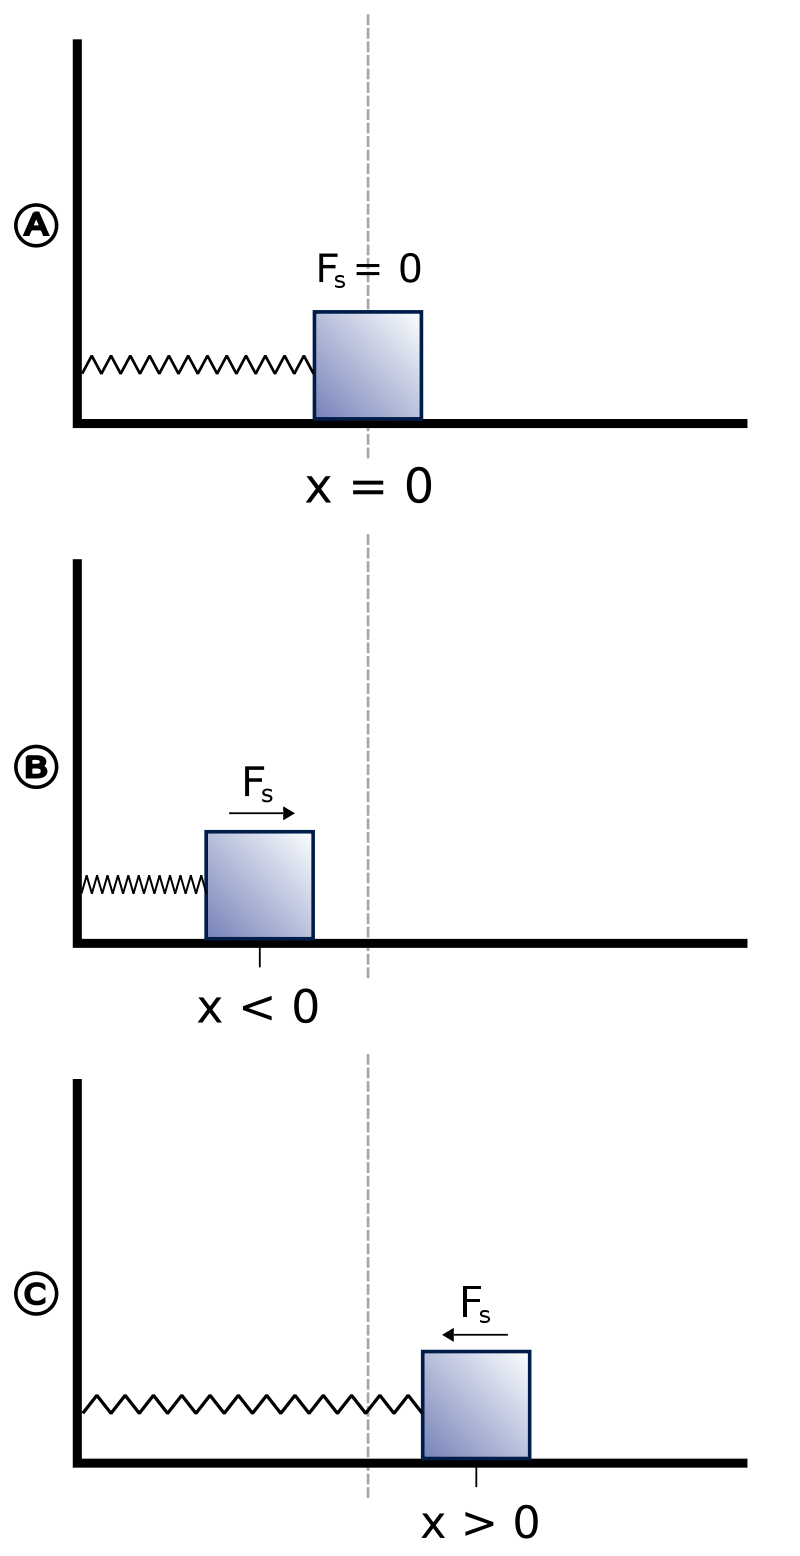
\includegraphics[width=.4\textwidth]{Figures/spring-mass.png}
            \caption{Spring-Mass system in the new variables. The dashed line represents the rest length $L$.}
            \label{fig:my_label}
        \end{figure}
        \end{ex}
        
        \begin{exercise}
        Show that
        \[
        y(t) = A\sin\left(\sqrt{\frac{k}{m}}t\right)+B\cos\left( \sqrt{\frac{k}{m}}t\right)
        \]
        solves the above differential equation.
        \end{exercise}
        
        \section{Separable ODE}
        The nicest possible ODE come from equations that are \emph{separable}.  What this means is that, for example, we have a first order equation like
        \[
        f'(t)=g(t)h(f(t)).
        \]
        Why is this nice? Well, in particular, it means that we can simply integrate this equation to solve it.  Many systems exhibit symmetry that allows for this type of separation, so this technique is crucial.
        
        In general, we have
        \[
        f'(t)=\frac{df}{dt}
        \]
        and we put
        \begin{align*}
            \frac{df}{dt}&=g(t)h(f(t))\\
            \iff \frac{1}{h(f(t))}df &= g(t)dt.
        \end{align*}
        With this, we can integrate both sides, then solve for $f$.  
        
        \begin{ex}{Separable ODE}{separable}
        Consider the following ODE
        \[
        f'(t)=\frac{t}{f(t)}. 
        \]
        Then we can put
        \begin{align*}
            \frac{df}{dt}&= \frac{t}{f}\\
            \iff fdf &= t dt.
        \end{align*}
        Then we can take the antiderivative of both sides and find
        \begin{align*}
            \int fdf &= \int t dt\\
            \iff \frac{1}{2}f^2 &= \frac{1}{2}t^2 + C\\
            \iff f(t)&=\sqrt{t^2+2C}.
        \end{align*}
        So now we can verify that this is in fact a solution to our ODE.  So we take
        \[
        f'(t) = \frac{d}{dt}\sqrt{t^2+2C}= \frac{t}{\sqrt{t^2+2C}} = \frac{t}{f(t)}.
        \]
        \end{ex}
        
        \begin{exercise}
        Solve the following ODE using separation
        \[
        f'(t)=t.
        \]
        Note that there will be an undetermined constant that we will learn how to handle next.
        \end{exercise}
        
        \section{Particular Solutions}
        In all previous examples, there were undetermined constants.  These constants appear since fundamentally an antiderivative is determined up to a constant.  Though not all ODE are solvable by direct integration, the constants are there due to this reason.
        
        How do we determine the constants?  It turns out we need a bit more information.  The extra information is also very intuitive and physical.  Take for example, a simplified version of the harmonic oscillator (spring-mass) system
        \[
        x''(t) = -x(t).
        \]
        Notice, we have just removed the constants.  This is always possible to do by picking the right way to measure the problem! Then I stated that the \emph{general solution} to this ODE is
        \[
        x(t)=A\sin(t) + B \cos (t).
        \]
        But, we don't know $A$ and $B$.  
        
        \begin{df}{General Solution}{gen_soln}
            A \textbf{general solution} to an $n$th order ODE is a solution with $n$  (call these values $c_1,c_2,\dots,c_n$) undetermined constants. A general solution is in fact a whole family of solutions. That is, there is a solution for each different value of the constants $c_1$, $c_2$, $\dots$, $c_n$.
        \end{df}
        
        If we think about the situation, we have just determined the general oscillatory behavior of the system, but not the any particular \emph{trajectory} of the system. What we need to know is where we pulled the mass to at the initial time $t=0$. That is, we need
        \[
        x(0)
        \]
        but we also need to know how fast it was moving at that point 
        \[
        x'(0).
        \]
        The analogy is as follows: If one is throwing a ball, one needs to know where it is released $\mathbf{x}(0)$, and the velocity at which it is released at $\mathbf{x}(0)$ in order to know where the ball will land.
        \begin{figure}[H]
            \centering
            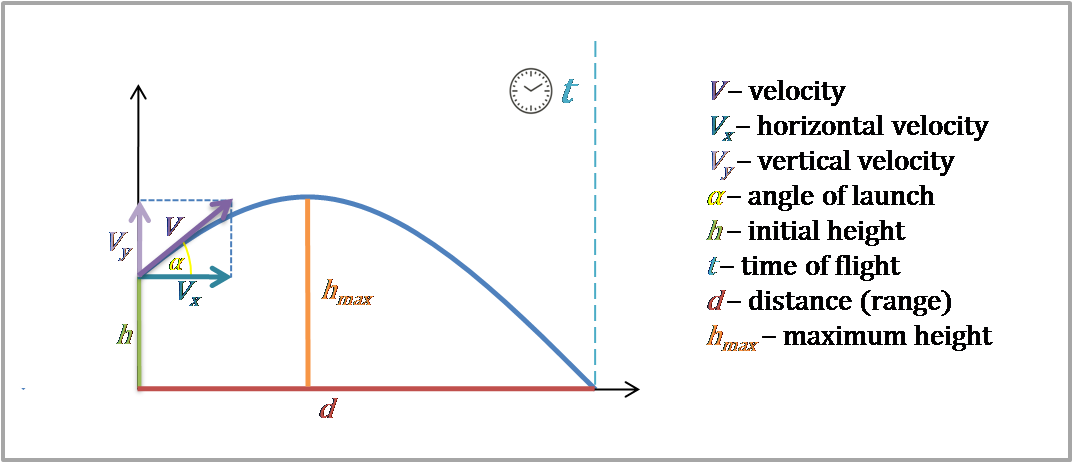
\includegraphics[width=.7\textwidth]{Figures/projectile-motion.png}
            \caption{Throwing a ball as an example of needing initial data.}
            \label{fig:my_label}
        \end{figure}
        We call these values $x(0)$ and $x'(0)$ the \emph{initial data}. 
        
        \begin{df}{Initial Data}{df: initial_data}
            The \textbf{initial data} to an $n$th order ODE are the specific values for
            \[
            x(0),~ x'(0),\dots,~ x^{(n-1)}(0),
            \]
            where $x^{(k)}$ represents the $k$th derivative of $x(t)$.
        \end{df}
        
        \begin{df}{Particular Solution}{particular_solution}
            A \textbf{particular solution} is one member of the family of general solutions.  That is, a solution where the constants $c_1,~c_2,\dots,~c_n$ are all uniquely determined.
        \end{df}
        
        \begin{prop}{Initial Data and Particular Solutions}{initial_data_part_solns}
        In order to find a particular solution to an $n$th order ODE, one needs to know the initial values of the function, its derivative, its second derivative, and all derivatives up to the $(n-1)th$ derivative
        \[
        x(0),~ x'(0),\dots,~ x^{(n-1)}(0).
        \]
        \end{prop}
        
        
        
        \begin{ex}{Particular Solution to Harmonic Oscillator}{part_soln_harm_osc}
        Consider 
        \[
        x''(t)=-x(t)
        \]
        with initial data
        \[
        x(0)=1, ~ x'(0)=0.
        \]
        This has the general solution
        \[
        x(t)=A \sin(t) + B \cos (t).
        \]
        We can find the particular solution by
        noting we have
        \[
        x(0)=A\sin(0)+B\cos(0)=1
        \]
        from our initial data.  Specifically, this gives us that
        \[
        B=1.
        \]
        Then note we also have
        \[
        x'(0)=A\cos (0) - \sin (0)=0
        \]
        which gives us that
        \[
        A=0.
        \]
        So our particular solution is
        \[
        x(t)=\cos (t).
        \]
        \end{ex}
        
        \subsubsection{Determinism}
        The reason why we study these differential systems is to make predictions and models.  Given that, our predictions must be sensible. This means if we are given a differential equation and initial data, there should only be one particular solution.  This is known as \textbf{determinism}.  
        
        Not all systems are deterministic.  But it turns out the non-deterministic systems are either problematic as models or just very hard to deal with.
        
        When solving an ODE, we call a particular solution a \textbf{trajectory}.
        
        
        \section{Projectile Motion}
        Above, we saw the example picture of projectile motion.  We have all thrown a ball, and we know what the motion looks like.  Let us derive exactly the equations of motion of a thrown ball and then a specific trajectory.
        
        \begin{ex}{Projectile Motion in 1D}{1d_proj_motion}
        Here we will start from a physical postulate, create a differential equation model, solve the model in general, then in particular, and lastly plug in exact values and units.
        
        \noindent \textbf{Problem Statement:} \emph{Near Earth, gravity is constantly forcing objects to accelerate downward at a constant rate $g=9.8m/s^2$. What is the trajectory of a ball with mass $5kg$ thrown straight upward from a height of $1m$ with initial velocity $10m/s$?}
        
        Since we only care about the ball moving straight up and down, we need only describe the height.  We let the height be given by $z(t)$ and acceleration is then the second derivative of height $z''(t)$.  We are told that the acceleration is downward at some constant rate, say $g$.  It turns out, the mass does not change this acceleration and we arrive at the equation
        \[
        z''(t)=-g
        \]
        where the minus sign tells us the object accelerates downward.
        
        It turns out this equation is separable, but requires a bit more care.  Note we have
        \[
        \frac{d^2z}{dt^2}=\frac{d}{dt}\frac{dz}{dt}=-g.
        \]
        The fundamental theorem of calculus says that we can take the antiderivative of this equation and get
        \[
        \frac{dz}{dt}=-g+C_1.
        \]
        Now we separate and integrate,
        \[
        \int dz = \int (-gt+C_1)dt
        \]
        and get
        \[
        z= -\frac{1}{2}gt^2+C_1t+C_2.
        \]
        So our general solution is
        \[
        z(t)=-\frac{1}{2}gt^2+C_1t+C_2.
        \]
        
        Then, say we are given initial data
        \[
        z(0)=z_0 \qquad z'(0)=z_1
        \]
        then using our general solution we have
        \[
        z(0)=-\frac{1}{2}g(0)^2+C_1(0)+C_2=z_0
        \]
        so 
        \[
        C_2=z_0.
        \]
        Then we can again use the general solution and get
        \[
        z'(0)=-g(0)+C_1 = z_1
        \]
        so
        \[
        C_1 = z_1.
        \]
        So our particular solution is then
        \[
        z(t) = -\frac{1}{2}gt^2 + z_1 t + z_0.
        \]
        
        Looking again at our problem statement, we are given that our initial height is
        \[
        z(0)=1m=z_0
        \]
        and the initial velocity is
        \[
        z'(0)=10m/s = z_1,
        \]
        So with our specific problem, the \textbf{trajectory} is
        \[
        z(t)=-\frac{1}{2}(9.8)t^2 + 10t+1.
        \]
        Here is the plot of this trajectory.
        \begin{figure}[H]
            \centering
            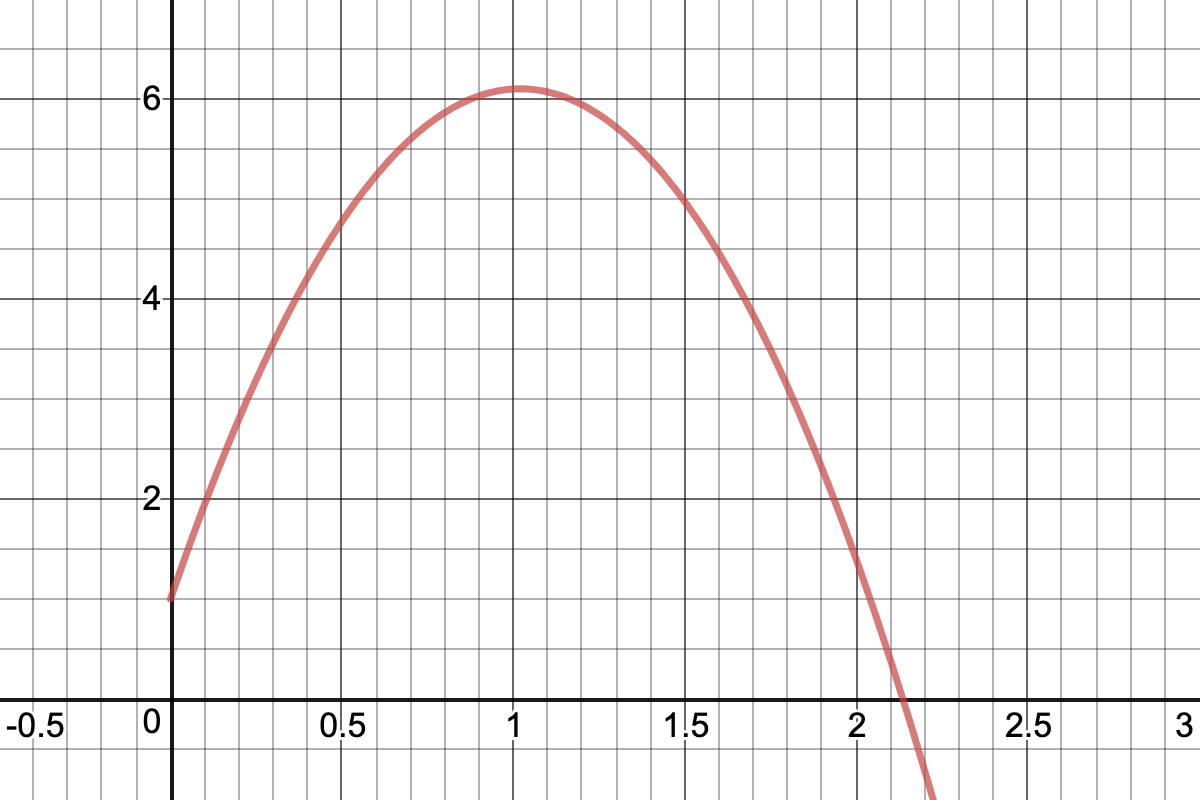
\includegraphics[width=.7\textwidth]{Figures/projectile_example.png}
            \caption{The trajectory of our example ball.}
            \label{fig:my_label}
        \end{figure}
        Notice that at some point this ball would go below the ground!  Our models aren't all knowing.  You would have to impose more information on the problem to say that the ball cannot go through $z=0$!  This goes to show that our models tend to only work over a short span in time. Even for a relatively simple problem like throwing a ball, we still have issues.
        \end{ex}
        
        \section{Exact Equations}
        
        To extend to a slightly larger class of equations, we consider one more type of first order equation.  These are the \emph{exact} equations.  These are differential equations that are much like the potential functions we saw in Part II.  We are given an equation
        \[
        P(x,t)dx + Q(x,t)dt = 0.
        \]
        Note that this is equivalent to a first order differential equation by rearranging
        \begin{align*}
            P(x,t)dx+Q(x,t)dt &= 0 \\
            \iff P(x,t)dx &= - Q(x,t)dt\\
            \iff \frac{dx}{dt} &= \frac{-Q(x,t)}{P(x,t)}\\
            \iff x' &= f(x,t).
        \end{align*}
        Exact equations make their appearance often in thermodynamics (with entropy, for example) but are in fact very far reaching.  One can understand complicated \emph{partial differential equations} by generalizing this concept.
        
        \begin{df}{Exact ODE}{exact}
        A first order equation 
        \[
        P(x,t)dx + Q(x,t)dt = 0
        \]
        is \textbf{exact} if there exists an $F(x,t)$ such that
        \[
        \frac{\partial F}{\partial x}= P(x,t) \quad \textrm{and} \quad \frac{\partial F}{\partial t}= Q(x,t).
        \]
        \end{df}
        
        \begin{prop}{An Equivalent Definition for Exactness}{exactness_equivalent}
        A first order equation
        \[
        P(x,t)dx + Q(x,t)dt = 0
        \]
        is exact if and only if
        \[
        \frac{\partial P}{\partial t}-\frac{\partial Q}{\partial x}=0.
        \]
        \end{prop}
                
        We can solve an exact equation in an analogous way to solving for a potential function.  Let us see where this comes from a bit.
        
        Let's say we have a function $F(x,t)$.  Then, the level curves of this function $F(x,t)=c$ can be thought of as trajectories!  
        
        \begin{ex}{Exact: Forward and Back}{exact_forward_back}
        \noindent \textbf{Forward:}
        Let's consider the function
        \[
        F(x,t) = x^2+t^2.
        \]
        Then a level curve is given by
        \[
        F(x,t)=x^2+t^2 = c
        \]
        which is a circle of radius $\sqrt{c}$.  Often times knowing this is the closed trajectory is enough.  For example, in the case for finding orbits of the planets.
        
        Then we can take what is called the \emph{differential} of both sides
        \begin{align*}
        dF(x,t)&=dc\\
        \implies \frac{\partial F}{\partial x}dx + \frac{\partial F}{\partial t}dt &= 0.
        \end{align*}
        Now, with our particular case we have
        \[
        2xdx+2tdt = 0.
        \]
        Is this equation exact? Yes, by definition, it is.  But we should verify with the proposition.  So we let
        \[
        P(x,t) = 2x \quad \textrm{and} \quad Q(x,t) = 2t
        \]
        and compute the partial derivatives
        \[
        \frac{\partial P}{\partial t} = 0 \quad \textrm{and} \quad \frac{\partial Q}{\partial x} = 0
        \]
        so indeed this proposition holds.
        
        \noindent \textbf{Back:} Say we were given
        \[
        2xdx+2tdt = 0, 
        \]
        how do we recover $F(x,t)$?  Can we recover it exactly?  Let's see.
        
        Here we can integrate the $dx$ term with respect to $x$ and determine a function up to an additional $f(t)$
        \[
        \int 2xdx = x^2 + f(t).
        \]
        Similarly, we can integrate the $dt$ term with respect to $t$ and find
        \[
        \int 2tdt = t^2 + g(x).
        \]
        Combining these two, we find that we have
        \[
        H(x,t) = x^2+t^2+c.
        \]
        However, we cared just about the level curves of this function so really, we recover
        \[
        x^2+t^2=c.
        \]
        \end{ex}
    
        \chapter{Systems of ODE}
        Though ODE consist of a single variable, it's possible that many ODE interact with each other and form a system.  Another case of interest would be finding trajectories as curves in higher dimensions (usually 2 or 3 for physical problems).  In this case we say that we have an \emph{system of ODE}.  
        
        For example, a system of three first order ODEs takes the form
        \begin{align*}
            x' &= f(x,y,z,t),\\
            y' &= g(x,y,z,t),\\
            z' &= h(x,y,z,t).
        \end{align*}
        
        \begin{df}{System of ODE}{system_of_ode}
            A \textbf{system of ODE} is a collection of differential equations of various order.  We call the system \textbf{coupled} if one of the differential equations is dependent on another.
        \end{df}
        
        \begin{ex}{SIR Model in Ecology}{sir_model}
        A biological example of a system of first order equations comes from modeling the spread of disease in a colony.  We let $S(t)$ denote the number of susceptible animals, $I(t)$ denote the number of infected animals, and $R(t)$ denote the animals resistant to the disease.  The model is a system of ODE of the form
        \begin{align*}
            S' &= -\frac{\beta IS}{N},\\
            I' &= \frac{\beta I S}{N} - \gamma I,\\
            R' &= \gamma I.
        \end{align*}
        We let $N=S(t)+I(t)+R(t)$ denote the constant population, and $\beta$ and $\gamma$ are other measured parameters.
        
        This is a coupled system since, for example, the equation $S'$ contains the function $I$.  We also see that the equation for $I'$ contains the function $S$.  Lastly, the equation for $R'$ contains the function $I$.  
        \end{ex}
        
 
        
        \section{Qualitative Analysis}
        The great part about a system of first order ODEs is that we can analyze them pictorially. 
        
        \begin{ex}{Zoo of First Order Linear Systems}{first_order_zoo}
        Let's consider the following systems.
        
        \begin{enumerate}[(I)]
            \item 
            \begin{align*}
                x' = x+y,\\
                y' = x+y.
            \end{align*}
            What we can do is put $x'$ and $y'$ into a vector 
            \[
            \mathbf{v}' = \begin{bmatrix} x' \\ y' \end{bmatrix}.
            \]
            This is actually a vector field $\mathbf{v}'(x,y)$!  We can plot this vector field and analyze from there.
            \begin{figure}[H]
                \centering
                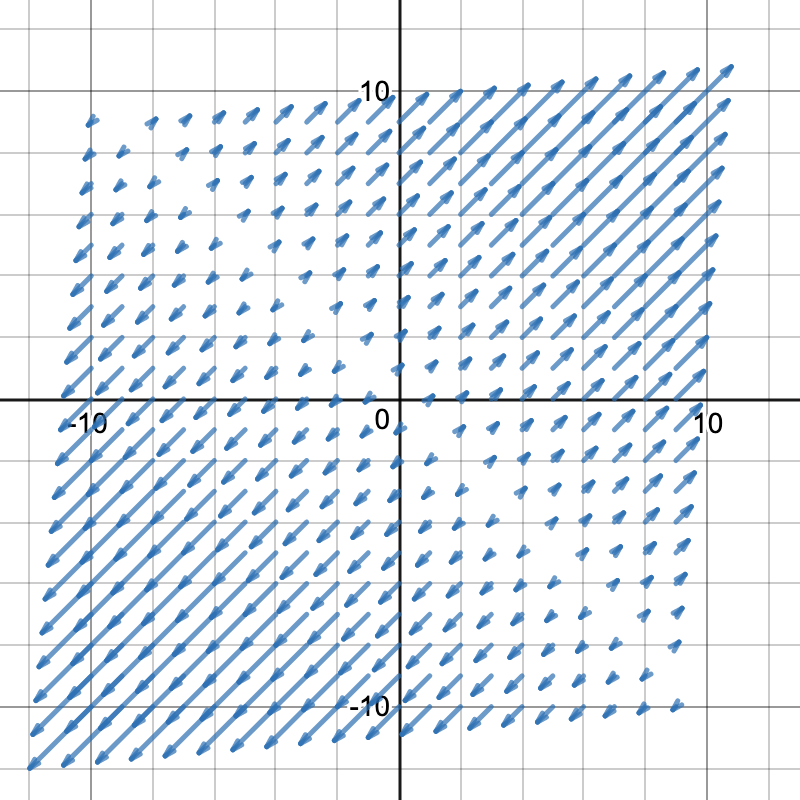
\includegraphics[width=.6\textwidth]{Figures/x+yx+y.png}
                \caption{A plot of the vector field $\mathbf{v}'(x,y)$.}
            \end{figure}
            Our goal is to then find a vector as a function of time given by
            \[
            \mathbf{v}(t) = \begin{bmatrix} x(t) \\ y(t) \end{bmatrix}
            \]
            as this will contain the solutions to our system of ODE.
            
            What we do next is pick an initial condition, $(x_0,y_0)$ and note that our vector field gives us the velocity vector $\mathbf{v}'(x_0,y_0)$ at that point. 
            
            The solution (curve/trajectory) to our system of ODE follows the vector field above since it describes the velocity of our curve at that point. We call this solution curve an \textbf{integral curve} as it is obtained (roughly) through integration of $\mathbf{v}'$.  However, you should know that it is not always possible to explicitly compute this integral.  We will learn techniques for solving certain systems, however.
            
            One should feel comfortable tracing an estimate for a solution curve for a given system as it gives a qualitative answer to the problem. In this case, if we pick a point along the line $y=-x$, the trajectory is stationary.  Otherwise, the solution follows a curve that is parallel to the $y=x$ line and the direction depends on which location it begins.
            \item We can repeat this process for another example
            \begin{align*}
                x' &= x+y,\\
                y' &= -x +y.
            \end{align*}
            This has a vector field plot:
            \begin{figure}[H]
                \centering
                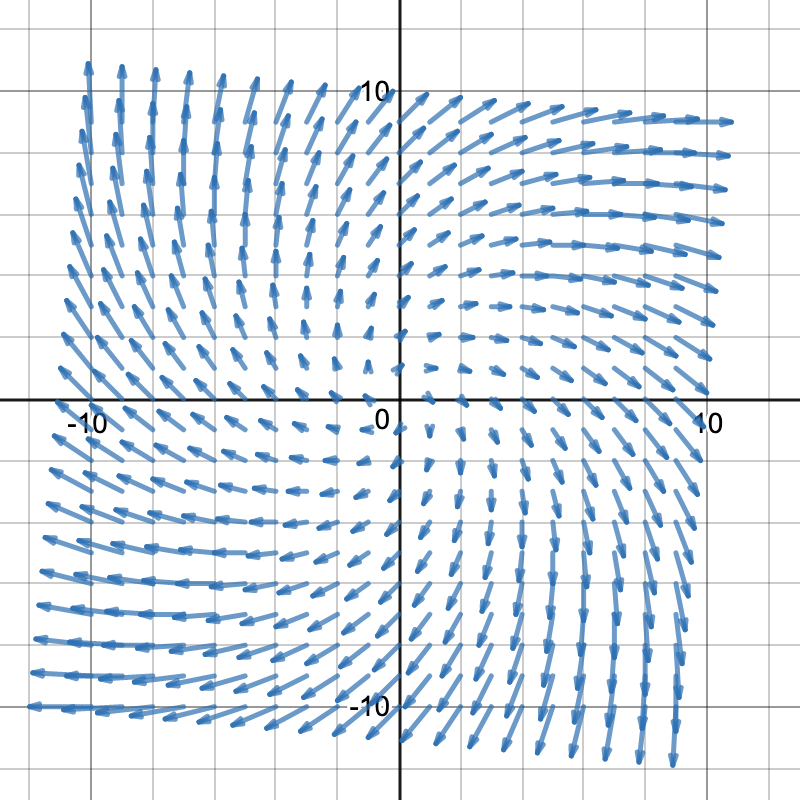
\includegraphics[width=.6\textwidth]{Figures/x+yx-y.png}
                \caption{The vector field $\mathbf{v}'(x,y)$ given by our system.}
                \label{fig:my_label}
            \end{figure}
            This solution has a stationary trajectory at the point $(0,0)$. Otherwise, the solution spirals outward in a clockwise direction. We say that this \emph{stationary point} $(0,0)$ is \emph{unstable}.
            \item Here is another example given by
            \begin{align*}
                x' &= -x +y,\\
                y' &= -x -y.
            \end{align*}
            Here is the plot of the vector field
            \begin{figure}[H]
                \centering
                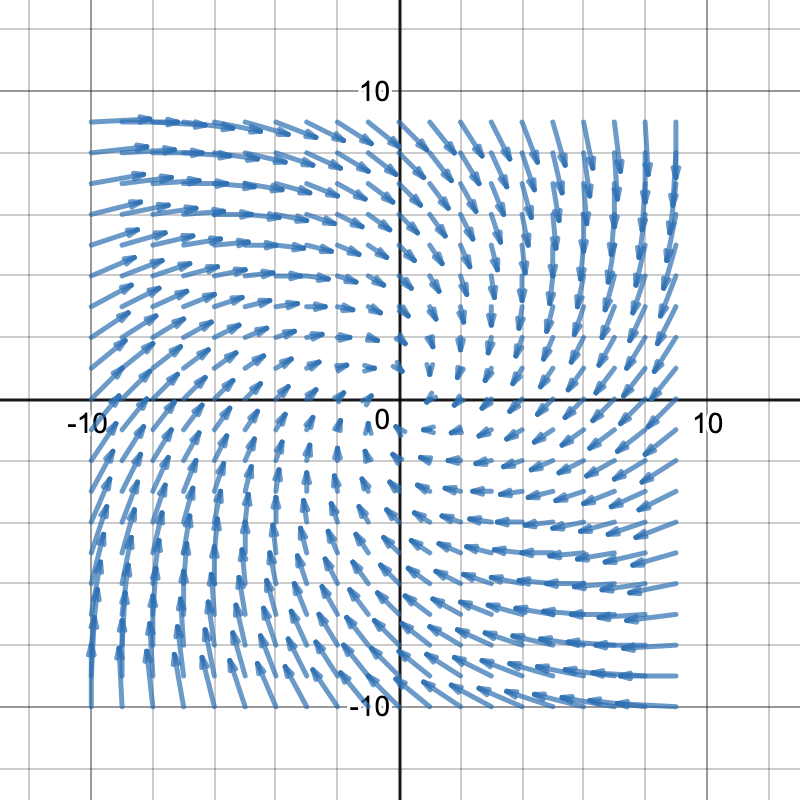
\includegraphics[width=.6\textwidth]{Figures/-x+y-x-y.png}
                \caption{The vector field $\mathbf{v}'(x,y)$ given by our system.}
                \label{fig:my_label}
            \end{figure}
            Here our solution again has a stationary trajectory at the point $(0,0)$.  Otherwise, the solution spirals inward in a clockwise direction.  Here we say that the stationary point $(0,0)$ is \emph{stable}.
            \item Let us take yet another example given by
            \begin{align*}
                x' &= y,\\
                y' &= -x.
            \end{align*}
            This has a vector field plot
            \begin{figure}[H]
                \centering
                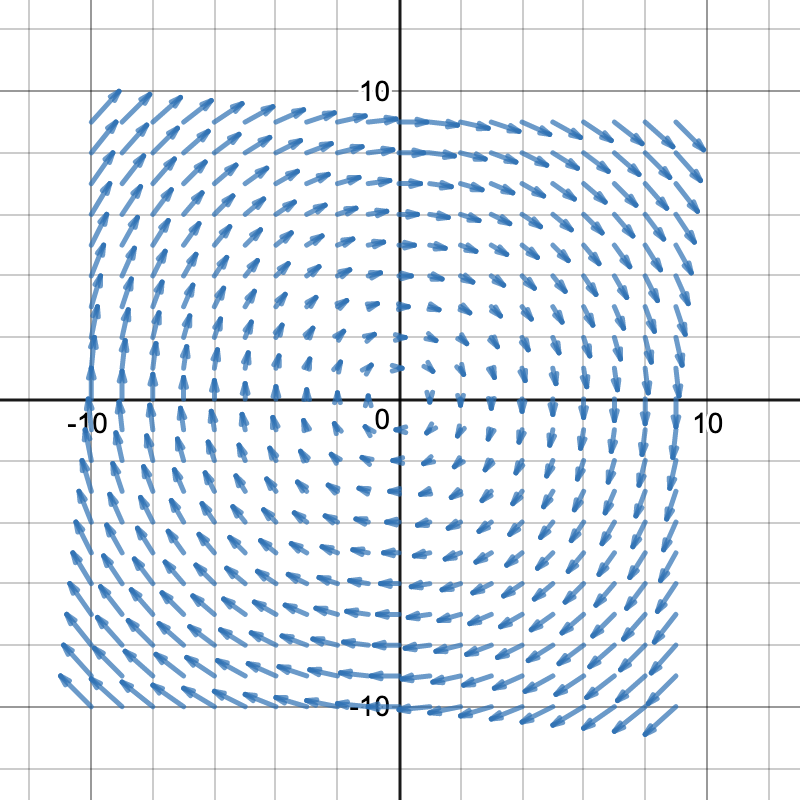
\includegraphics[width=.6\textwidth]{Figures/y-x.png}
                \caption{The vector field $\mathbf{v}'(x,y)$ given by our system.}
                \label{fig:my_label}
            \end{figure}
            Again, $(0,0)$ is a stationary point.  All the other trajectories form circles that rotate counter clockwise about the origin.
        \end{enumerate}
        \end{ex}
        
        These systems above show the four main dynamics we can see in the plane. All dynamics in the plane roughly look like one of these in close proximity to any point.
        
        \begin{ex}{General Solutions to the Zoo of Linear Systems}{gen_solns_zoo}
        We can look at the integral curves for these vector fields.  Without solving them explicitly, let's see what they would look like.
        \begin{enumerate}[(I)]
            \item The general solution for this system is
            \begin{align*}
                x(t)&= \frac{1}{2}c_1 \left( e^{2t}+1\right)+\frac{1}{2}c_2\left(e^{2t}-1\right),\\
                y(t)&=\frac{1}{2}c_1 \left( e^{2t}-1\right)+\frac{1}{2}c_2\left(e^{2t}+1\right).
            \end{align*}
            The initial data is dictated by the problem, and comes in the form of knowing $(x(0),y(0))$.  Here is a plot of a few integral curves (trajectories).
            \begin{figure}[H]
                \centering
                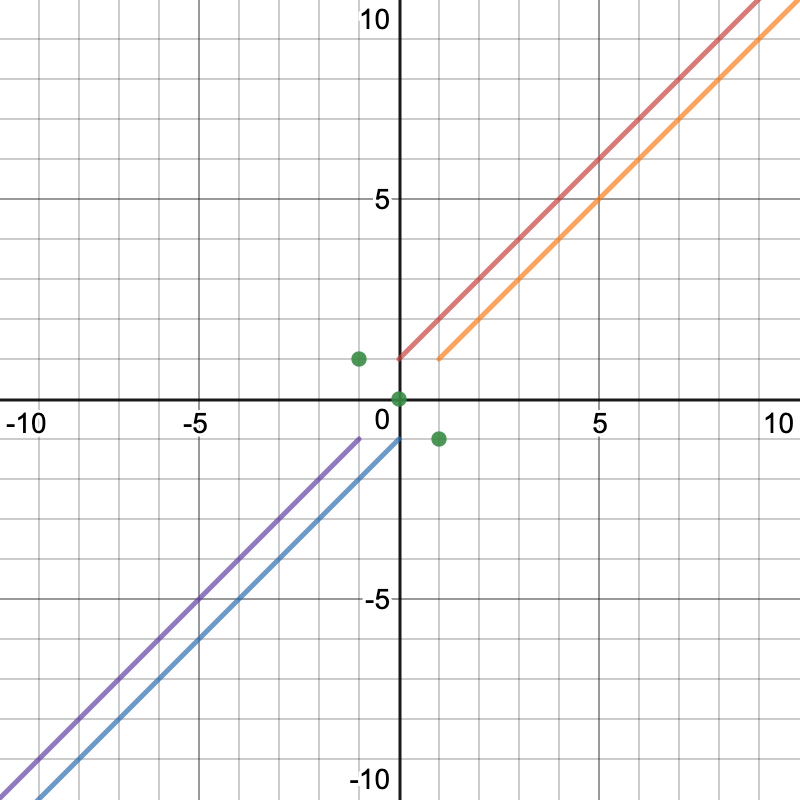
\includegraphics[width=.6\textwidth]{Figures/x+yx+yintegralcurves.png}
                \caption{Integral curves. Red: $(0,1)$; Orange: $(1,1)$; Purple: $(-1,-1)$; Blue: $(0,-1)$. Green are all stationary points.}
                \label{fig:my_label}
            \end{figure}
            \item The general solution for this system is
            \begin{align*}
                x(t)&= c_2 e^t \sin(t)+c_1e^t\cos(t),\\
                y(t)&= c_2 e^t \cos(t) - c_1e^1 \sin(t).
            \end{align*}
            Here are trajectories. Keep in mind these move radially \emph{outward} away from the stationary point!
                        \begin{figure}[H]
                \centering
                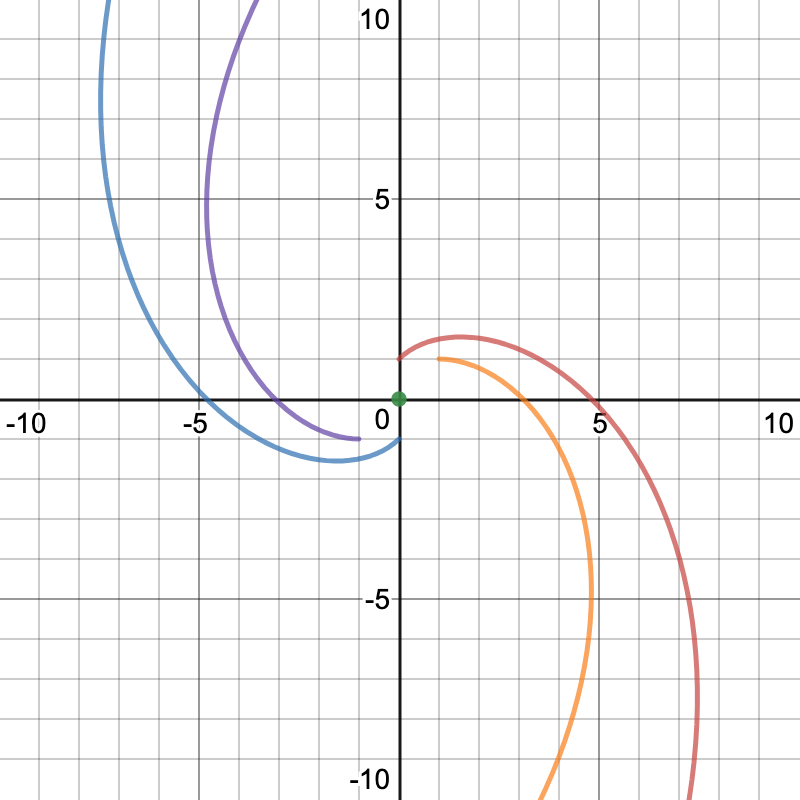
\includegraphics[width=.6\textwidth]{Figures/x+y-x+yintegralcurves.png}
                \caption{Integral curves. Red: $(0,1)$; Orange: $(1,1)$; Purple: $(-1,-1)$; Blue: $(0,-1)$. Green:$(0,0)$ is the stationary point.}
                \label{fig:my_label}
            \end{figure}
            \item The general solution for this system is
            \begin{align*}
                x(t)&=c_2 e^{-t}\sin(t)+c_1 e^{-t}\cos(t),\\
                y(t)&=c_2e^{-t}\cos(t)-c_1e^{-t}\sin(t).
            \end{align*}
            Here are trajectories. Keep in mind these are moving radially \emph{inward} towards the stationary point! Also note the difference in scale here.
            \begin{figure}[H]
                \centering
                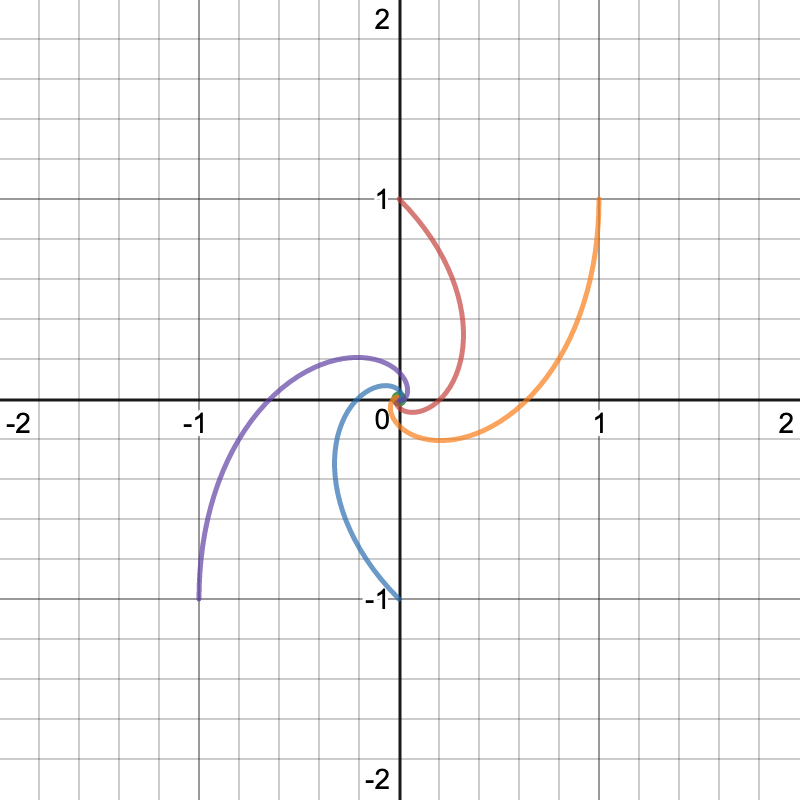
\includegraphics[width=.6\textwidth]{Figures/-x+y-x-yintegralcurves.png}
                \caption{Integral curves. Red: $(0,1)$; Orange: $(1,1)$; Purple: $(-1,-1)$; Blue: $(0,-1)$. Green: $(0,0)$ is the stationary point.}
                \label{fig:my_label}
            \end{figure}
            \item The general solution for this system is
            \begin{align*}
                x(t)&= c_2 \sin(t) + c_1 \cos(t),\\
                y(t)&= c_2 \cos(t) - c_1 \sin(t).
            \end{align*}
            Some of the trajectories here end up overlapping if we plot them over too much time.  Here's what I mean.
            \begin{figure}[H]
                \centering
                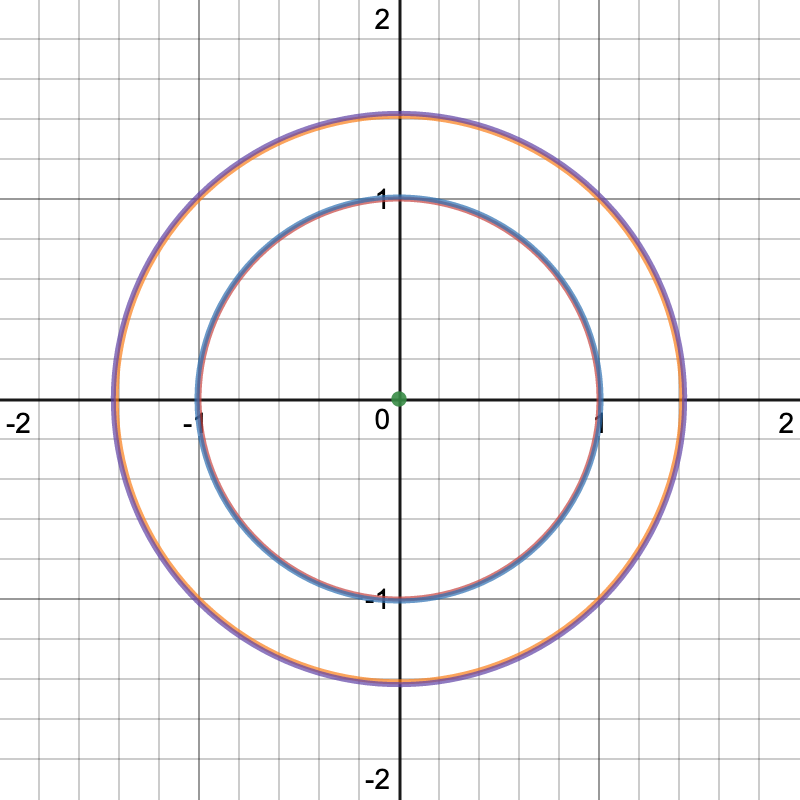
\includegraphics[width=.6\textwidth]{Figures/y-xintegralcurves.png}
                \caption{Integral curves. Red: $(0,1)$; Orange: $(1,1)$; Purple: $(-1,-1)$; Blue: $(0,-1)$. Green: $(0,0)$ is the stationary point.}
                \label{fig:my_label}
            \end{figure}
            However, here is what it looks like over a shorter period of time.
            \begin{figure}[H]
                \centering
                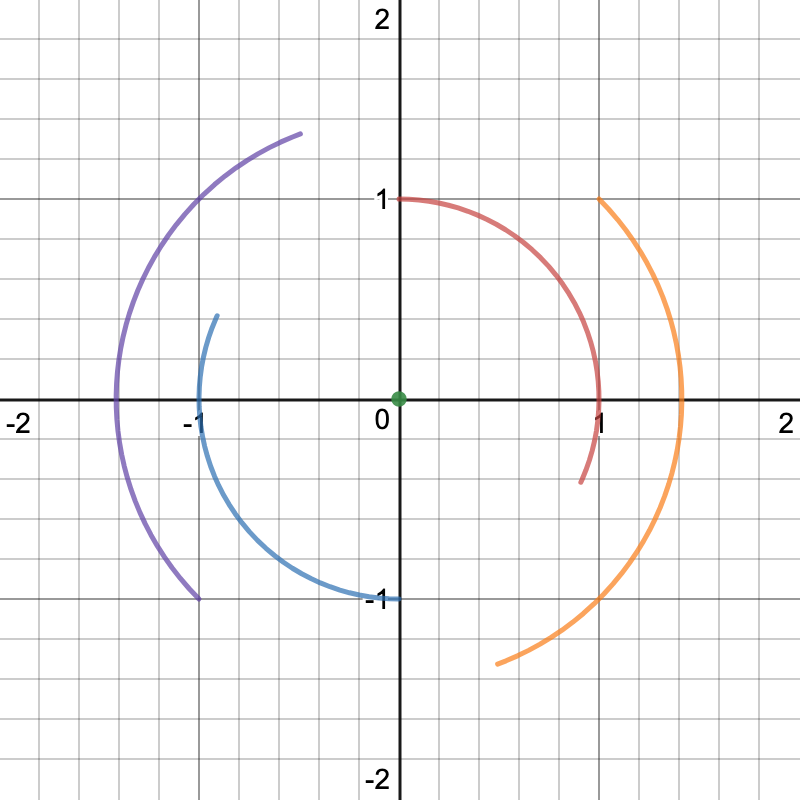
\includegraphics[width=.6\textwidth]{Figures/y-xintegralcurves2.png}
                \caption{Integral curves. Red: $(0,1)$; Orange: $(1,1)$; Purple: $(-1,-1)$; Blue: $(0,-1)$. Green: $(0,0)$ is the stationary point.}
                \label{fig:my_label}
            \end{figure}
            In a sense, each chosen initial conditions will chase one of the others forever in time.
        \end{enumerate}
        \end{ex}
        
        \section{Linearity}
        The above systems were all \emph{linear}.  These systems are in fact exactly solvable.  We'll get to the solutions shortly.  However, many systems in nature are \emph{nonlinear}.  Take for example, the SIR model. What does it mean for an ODE to be linear? 
        
        \begin{df}{Linear and Nonlinear ODE}{lin_ode}
        An $n$th order ODE is \textbf{linear} if it can take the following form
        \[
        x^{(n)}(t)+f_{n-1}(t)x^{(n-1)}(t)+\cdots + f_1(t)x'(t) +f_0(t)x(t)=g(t).
        \]
        This looks a bit complicated, so let's restate this for second order ODE.
        
        A second order $ODE$ is \textbf{linear} if it can take the following form
        \[
        x''+f(t)x'+g(t)x=h(t).
        \]
        And a first order ODE is linear if it can take the form
        \[
        x'+f(t)x=g(t).
        \]
        
        If an ODE does not satisfy the above definition, we say that it is \textbf{nonlinear}.
        \end{df}
        
        
        \section{Higher Order ODE}
        Higher order ODE show up in nature quite often.  For example, second order equations are abundant in physics due to Newton's laws.  Equations of order higher than two appear in material strain and stress (which tend to be fourth order).  
        
        The wonderful fact is that we do not need any new theory to understand higher order ODE.  This is due to the following theorem.
        
        \begin{thm}{Reduction of Order}{red_of_order}
        Any $n ^\textrm{th}$ order ODE is equivalent to a system of $n$ first order ODE.  
        \end{thm}
        
        The moral is that we need only know how to analyze first order systems in order to understand \emph{any} possible ODE.  Let's see an example of this.
        
        \begin{ex}{Order Reducing the Harmonic Oscillator}{order_red_harm_osc}
        Consider the harmonic oscillator equation
        \[
        x''=-x.
        \]
        We can define a new variable, $v$ so that $v=x'$.  Then note we have that $v'=x''$.  Substituting these gives us two first order equations
        \begin{align*}
            x'&=v,\\
            v'&=-x.
        \end{align*}
        It may seem like we have essentially done nothing.  But we've actually changed the problem for the better.  We'll see why soon.
        \end{ex}
        
        \begin{ex}{The Biharmonic Equation}{biharmonic_eq}
        Consider the \emph{biharmonic equation}
        \[
        x''''=x.
        \]
        We can define a set of new variables $y=x'$, $z=y'$, and $w=z'$.  Note that $w'=z''=y'''=x''''$. Then we arrive at the system
        \begin{align*}
            x'&=y,\\
            y'&=z,\\
            z'&=w,\\
            w'&=x.
        \end{align*}
        We have turned a fourth order ODE into a system of four first order ODE.
        \end{ex}
        
        \section{Linear Systems}
        Let's say we are given a nonlinear higher order ODE or system. We wish to be able to convert this to a linear problem of the form 
        \[
        \mathbf{v}'=A\mathbf{v}+\mathbf{F}
        \]
        where, for example, 
        \[
        \mathbf{v}=\begin{bmatrix} x(t) \\ y(t) \\ z(t) \end{bmatrix} \qquad \mathbf{v}'=\begin{bmatrix} x'(t) \\ y'(t) \\ z'(t) \end{bmatrix} \qquad \begin{bmatrix} f_1(t) \\ f_2(t) \\ f_3(t) \end{bmatrix}.
        \]
        We call this the \emph{inhomogeneous} system. 
        
        Roughly speaking, we can think of $\mathbf{F}$ as an external forcing term acting on the system.  We will concentrate more on solving the case where $\mathbf{F}=\mathbf{0}$ so that we have
        \[
        \mathbf{v}'=A\mathbf{v}.
        \]
        We call this the \emph{homogeneous} system. Here, $A$ is a $3\times 3$-matrix whose coefficients could possibly depend on time.  That is,
        \[
        A = \begin{bmatrix} A_{11}(t) & A_{12}(t) & A_{13}(t)\\
        A_{21}(t) & A_{22}(t) & A_{23}(t)\\
        A_{31}(t) & A_{32}(t) & A_{33}(t)\end{bmatrix}.
        \]
        We will ignore the case where the matrix depends on time and just work on the case where the coefficients are constant. This is called an \emph{autonomous} system.
        
        \begin{df}{Linear System of ODE}{linear_system}
            A system of first order differential equations is \textbf{linear} if it can be expressed as a matrix equation
            \[
            \mathbf{v}' = A(t)\mathbf{v}+\mathbf{F}(t).
            \]
            The linear system is said to have \textbf{constant coefficients} if the matrix $A(t)$ only contains constant.  That is, $A$ does not actually depend on $t$.
        \end{df}
        
        \begin{df}{Homogeneous and Inhomogeneous Linear Systems}{homogeneous_systems}
            A linear system of differential equations is 
            \textbf{inhomogeneous} if it can be expressed as
            \[
            \mathbf{v}' = A(t)\mathbf{v}+\mathbf{F}(t).
            \]
            If $\mathbf{F}(t)=0$ and we have
            \[
            \mathbf{v}' = A(t)\mathbf{v}
            \]
            then we say the system of differential equations is \textbf{homogeneous}.
        \end{df}
        
        \begin{df}{Autonomous}{autonomous}
        An \textbf{autonomous} first order system (in 3-dimensions) is given by the equations
        \begin{align*}
        x' &= f(x,y,z),\\
        y' &= g(x,y,z),\\
        z' &= h(x,y,z).
        \end{align*}
        This is autonomous due to the fact that $t$ does not appear as an argument for the functions $f,g,$ and $h$.
        \end{df}
        
        Autonomous systems are extremely common in reality which is why it is not a bad idea to emphasize them here.  These are the systems in which some quantity is being conserved over time, and hence the apparent $t$ dependence of the functions (shown above) is gone.  Of course, the functions still depend on $t$!  A few examples are
        \begin{itemize}
            \item mechanical systems (energy is conserved),
            \item closed thermodynamic systems (energy is conserved),
            \item short time ecologocial systems (animal number is conserved), 
            \item closed chemically reacting systems (total atomic count is constant).
        \end{itemize}
        
        For us, we are going to concentrate on dynamics for a system of two equations.  That is, equations that exist in the plane.  For one, these systems are easier to solve by hand than the higher dimensional systems.  They are also very common to see due again to Newton's laws.  Often, we will find we can decompose larger systems of equations into sets of systems of two equations. Lastly, these are likely the easiest to visualize and build intuition with.  
        
        \section{Linearization}
        If we are given a planar (autonomous) and possibly nonlinear system, 
        \begin{align*}
            x'&= f(x,y),\\
            y'&= g(x,y),
        \end{align*}
        we want to approximate this system with a homogeneous linear system with a matrix with constant coefficients.  That is
        \[
        \begin{bmatrix} x' \\ y' \end{bmatrix} \approx \begin{bmatrix} A_{11} & A_{12} \\ A_{21} & A_{22} \end{bmatrix} \begin{bmatrix} x \\ y \end{bmatrix}.
        \]
    
        Remember that what we have here is a 2-dimensional vector field given by our system
        \[
        \mathbf{v}(x,y) = \begin{bmatrix} f(x,y) \\ g(x,y) \end{bmatrix}.
        \]
        The best linear approximation to this vector field at a point $(x_0,y_0)$ is given by the Jacobian $J(x_0,y_0)$ for this vector field
        \[
        J(x_0,y_0) = \begin{bmatrix} \frac{\partial f}{\partial x}(x_0,y_0) & \frac{\partial f}{\partial y}(x_0,y_0) \\
        \frac{\partial g}{\partial x}(x_0,y_0) & \frac{\partial g}{\partial y}(x_0,y_0) \end{bmatrix}.
        \]
        We will then let the coefficient matrix be given by this Jacobian.  That is, we get
        \[
        \begin{bmatrix} x' \\ y' \end{bmatrix} = J(x_0,y_0)\begin{bmatrix} x \\ y \end{bmatrix}.
        \]
        Let's work an example.
        
        \begin{ex}{Lotka-Volterra Model Linearization}{lotka_volterra_linearization}
        Let us consider a predator and prey system given by the Lotka-Volterra model.  Here we let the number of prey be given by $R(t)$ and the number of predators be given by $S(t)$.  The system is
        \begin{align*}
            S' &= (-c+dR)S,\\
            R' &= (a-bS)R,
        \end{align*}
        where $a,b,c,d>0$. Here we can say that we have
        \begin{align*}
        f(S,R) &= (-c+dR)S,\\
        g(S,R) &= (a-bS)R.
        \end{align*}
        We compute each partial derivative
        \begin{align*}
            \frac{\partial f}{\partial S} &= -c+dR & \frac{\partial f}{\partial R} &=dS \\
            \frac{\partial g}{\partial S} &= -bR & \frac{\partial g}{\partial R} &= a-bS.
        \end{align*}
        Evaluating each at the point $(S_0,R_0)$ and placing into a matrix gives us the Jacobian
        \[
        J(S_0,R_0)=\begin{bmatrix} -c+dR_0 & dS_0 \\ -bR_0 & a-bS_0 \end{bmatrix}.
        \]
        
        Now, about this point, our system approximately takes the form
        \[
        \begin{bmatrix} S' \\ R' \end{bmatrix} = \begin{bmatrix} -c+dR_0 & dS_0 \\ -bR_0 & a-bS_0 \end{bmatrix} \begin{bmatrix} S \\ R \end{bmatrix}.
        \]
        \end{ex}
        
        Our goal now is to learn how we can explicitly solve these planar systems.  With that, we will be able to solve many problems.
        
        
        Now that we can take many common ODE, convert them to a system of first order ODE, and linearize the system, we can work to solve these specific equations.  The detail is captured by the following.
        
        \begin{prop}{Eigenfunction of the Derivative}{eigenfunction}
        The exponential function $e^{kx}$ is an \textbf{eigenfunction} for the derivative.  \\
        
        \noindent \emph{Proof.} We take 
        \[
        \frac{d}{dt} e^{kt} = ke^{kt}.
        \]
        So, the eigenvalue is $k$ for this eigenfunction. \qed
        \end{prop}
        
        
        Spending the time being more rigorous with this is an interesting endeavor, but we have done enough theoretical results for now.  Let us see an example.
        
        \begin{ex}{Harmonic Oscillator Eigenvalue}{harm_osc_eigen}
        If we take the Harmonic Oscillator equation
        \[
        x'' = -x
        \]
        we can realize this extremely similar to an eigen equation with
        \[
        x'=ix.
        \]
        So, this eigen equation has a solution
        \[
        x(t)=e^{it}.
        \]
        Note that this solves the Harmonic oscillator equation since
        \[
        \frac{d^2}{dt^2} x(t) = \frac{d}{dt}ie^{it} = -e^{it}=-x.
        \]
        Remember that
        \[
        e^{it}=\cos(t)+i\sin(t)
        \]
        which captures the oscillating behavior.
        \end{ex}
        
        In short, these exponential functions capture oscillations, growth, and decay.  With these functions, we can model all linear systems.
        
        \begin{prop}{General Solution to Planar Linear Systems}{gen_soln_lin_systems}
        Given a two dimensional linear system with constant coefficients $A,B,C$, and $D$,
        \begin{align*}
        x' &= Ax+By,\\
        y' &= Cx+Dy,
        \end{align*}
        we can write this as a matrix equation
        \[
        \begin{bmatrix} x' \\ y' \end{bmatrix} = \begin{bmatrix} A & B\\ C & D \end{bmatrix} \begin{bmatrix} x \\ y \end{bmatrix},
        \]
        with
        \[
        M=\begin{bmatrix} A & B \\ C & D \end{bmatrix}.
        \]
        Let $\lambda_1$ and $\lambda_2$ be the (complex) eigenvalues of $M$ and $\mathbf{v}_1$ and $\mathbf{v}_2$ be the corresponding eigenvectors.  Then, the solution to the system of equations is
        \[
        \begin{bmatrix} x(t) \\ y(t) \end{bmatrix} = c_1 \mathbf{v}_1 e^{\lambda_1t} + c_2 \mathbf{v}_2e^{\lambda_2 t}.
        \]
        \end{prop}
        
        Let us unravel this with an example problem.
        
        \begin{ex}{Damped Harmonic Motion}{damped_harm_motion}
        Consider the Damped Harmonic Oscillator equation
        \[
        x'' +\mu x' + kx = 0,
        \]
        with initial data $x(0)=1$ and $x'(0)=0$.\\ 
        
        Let us first think about this problem with our intuition.  This equation is modelling a spring mass system that is in a damping medium (i.e., underwater).  What happens as this system evolves?  One should expect oscillation, but will the system oscillate indefinitely? No.  One should expect that this system will also begin to oscillate with less intensity over time.  With this, one could hazard a guess that
        \[
        x(t) \approx e^{-t}\cos(t).
        \]
        
        We can reduce the order of this equation by letting $y=x'$.  This gives us the system
        \begin{align*}
        x' &= y,\\
        y' &= -kx -\mu y.
        \end{align*}
        So we can write this as a matrix equation
        \[
        \begin{bmatrix} x' \\ y' \end{bmatrix} = \begin{bmatrix} 0 & 1 \\ -k & -\mu \end{bmatrix}.
        \]
        For simplicity, let $k=\mu=1$, and we get the matrix
        \[
        M = \begin{bmatrix} 0 & 1 \\ - 1& - 1 \end{bmatrix}.
        \]
        Then the eigenvalues to this matrix are
        \[
        \lambda_1 = \frac{1}{2}(-1+i\sqrt{3})\quad \textrm{and} \quad \lambda_2 = \frac{1}{2}(-1-i\sqrt{3}).
        \]
        The eigenvectors are
        \[
        \mathbf{v}_1 = \begin{bmatrix} \frac{1}{2} (-1-i\sqrt{3}) \\ 1 \end{bmatrix} \quad \textrm{and} \quad \mathbf{v}_2 = \begin{bmatrix} \frac{1}{2} (-1+i\sqrt{3}) \\ 1 \end{bmatrix}.
        \]
        By the proposition, our solution is
        \[
        \begin{bmatrix} x(t) \\ y(t) \end{bmatrix} = c_1 \begin{bmatrix} \frac{1}{2} (-1-i\sqrt{3}) \\ 1 \end{bmatrix} e^{\frac{1}{2}(-1+i\sqrt{3})t}+c_2  \begin{bmatrix} \frac{1}{2} (-1+i\sqrt{3}) \\ 1 \end{bmatrix} e^{\frac{1}{2}(-1-i\sqrt{3})t}.
        \]
        However, in this case we are wishing to just find $x(t)$ that fits this data, and what we find is this system of equations reduces to
        \begin{align*}
        x(t) &= c_1 e^{\frac{1}{2}(-1+i\sqrt{3})t}+c_2 e^{\frac{1}{2}(-1-i\sqrt{3})t},
        \end{align*}
        by looking at just the first entry of each vector and realizing that since $c_1$ and $c_2$ are undetermined constants, we can remove the other constants that appear.
        
        Now, let's use Euler's formula, and we have
        \begin{align*}
            x(t) &= c_1 e^{\frac{1}{2}(-1+i\sqrt{3})t}+c_2 e^{\frac{1}{2}(-1-i\sqrt{3})t}\\
            &= c_1 e^{-t/2}\left(\cos\left(\frac{\sqrt{3}}{2}t\right)+i\sin\left(\frac{\sqrt{3}}{2}t\right)\right)+c_2 e^{-t/2}\left(\cos\left(-\frac{\sqrt{3}}{2}t\right)+i\sin\left(-\frac{\sqrt{3}}{2}t\right)\right).
        \end{align*}
        There are a few more simplifications that can be done, but in the end we find the general solution
        \[
        x(t) = c_1 e^{-t/2} \sin\left(\frac{\sqrt{3}}{2}t\right)+c_2e^{-t/2}\cos\left(\frac{\sqrt{3}}{2}t\right).
        \]
        We were given that $x(0)=1$ and we have that
        \[
        x(0)=1=c_2
        \]
        by plugging into our general solution.  We also have that
        \[
        x'(0)=0=\frac{-\sqrt{3}}{4}c_1
        \]
        which means $c_1=0$.  So our particular solution is
        \[
        x_p(t) = e^{-1/2t}\cos \left(\frac{\sqrt{3}}{2}t\right).
        \]
        
        This solution also seems fit our physical expectations of the damped spring-mass system.  Great!
        \end{ex}
        
        \begin{exercise}
        Verify that this $x_p$ above is indeed a solution to the original ODE with $k=\mu=1$.
        \end{exercise}

        \begin{remark}
        The apparent difficulty of solving ODEs becomes obvious here.  In this extremely nice case it still took a large amount of work.  The case for other systems is generally worse.
        \end{remark}
        
        \section{General Solutions to Second Order Linear Equations}
        
        We can now write the general solutions to all second order linear equations.  We have the following.
        
        \begin{prop}{General Solutions to Second Order Linear Equations}{gen_solns_second_order}
        Given a second order homogeneous linear ODE
        \[
        x'' + \mu x' + kx = 0
        \]
        we can write this as a system of first order linear equations given by
        \[
        \mathbf{v}' = M \mathbf{v},
        \]
        where
        \[
        \mathbf{v} = \begin{bmatrix} x \\ y \end{bmatrix}.
        \]
        the eigenvalues of $M$ are either purely real or complex.
        
        \begin{itemize}
            \item If the eigenvalues $\lambda_1$ and $\lambda_2$ are complex, then the solution is
        \[
        x(t)= c_1 e^{\RE(\lambda_1)t} \sin(\IM(\lambda_1)t) + c_2 e^{\RE(\lambda_1)t} \sin(\IM(\lambda_1)t).
        \]
        It does not actually matter if we choose $\lambda_1$ or $\lambda_2$!
        \item         If the eigenvalues $\lambda_1$ and $\lambda_2$ are real then the general solution is:
        \[
        x(t) = c_1 e^{\lambda_1 t} + c_2 e^{\lambda_2 t}.
        \]
        \end{itemize}
        \end{prop}
        
        
% %%%%%%%%%%%%%%%%%%%%%%%%%%%%%%%%%%%%%%%%%%%%%%%%%%%%%%%%%%%%%%%%%%%%%%%%%%%%%%%%%%%%
% Partial Differential Equations
% %%%%%%%%%%%%%%%%%%%%%%%%%%%%%%%%%%%%%%%%%%%%%%%%%%%%%%%%%%%%%%%%%%%%%%%%%%%%%%%%%%%%
        
        \chapter{Partial Differential Equations}
        
        We now want to investigate a larger class of differential equations.  These are the \emph{partial differential equations} or PDE.  These equations become yet more complicated to solve, but are very prevalent in the study of the physical world.
        
        Fundamentally, these are time-varying differential equations of vector and scalar fields of many variables.  The goal for us is to be able to recognize a few specific example equations and understand their behavior.  We will also be able to solve a few equations with our tools from studying ODE. However, it is easy to pose a PDE that is virtually impossible to solve.  
        
        \begin{df}{Partial Differential Equation}{pde}
        A \textbf{partial differential equation of a scalar field} of three spatial variables $x,y,z$ and a time variable $t$ is an expression of a scalar function $u(x,y,z,t)$, the partial derivatives of $u(x,y,z,t)$, and other functions.
        \end{df}
        
        \begin{df}{Vector Partial Differential Equation}{vec_pde}
        A \textbf{partial differential equation of a vector field}
        \[
        \mathbf{v}(x,y,z,t) = \begin{bmatrix} v_1(x,y,z,t) \\ v_2(x,y,z,t) \\ v_3(x,y,z,t) \end{bmatrix}
        \]
        is an equation containing $\mathbf{v}$, the (component) derivatives of $\mathbf{v}$, and other vector fields.
        \end{df}
        
        With the difficulty of these expressions as is, we will concentrate solely on the equations with scalar functions.
    % %%%%%%%%%%%%%%%%%%%%%%%%%%%%%%%%%%%%%%%%%%%%%%%%%%%%%%%%%%%%%%%%%%%%%%%%%%%%%%%%%%%%
    % Examples of PDE
    % %%%%%%%%%%%%%%%%%%%%%%%%%%%%%%%%%%%%%%%%%%%%%%%%%%%%%%%%%%%%%%%%%%%%%%%%%%%%%%%%%%%%
    
        \section{Examples of PDE}
        
        \begin{ex}{Heat Equation}{heat_eqn}
        The \textbf{heat equation} in three dimensional space is the equation
        \[
        \frac{\partial u}{\partial t}(x,y,z,t) -k\nabla \cdot (\nabla u(x,y,z,t)) = f(x,y,z,t).
        \]
        This equation models the diffusion of heat in a region of space, hence the name.  In this case, we think of $u(x,y,z,t)$ being the temperature at the point $(x,y,z)$ at the time $t$.
        \end{ex}
        
        \begin{ex}{Laplace (Poisson) Equation}{laplace}
        The \textbf{Laplace} (sometimes \textbf{Poisson}) \textbf{equation} in three dimensional space is the equation
        \[
        -\nabla \cdot (\nabla u(x,y,z))=f(x,y,z).
        \]
        \emph{Notice, there is no dependence on time!} This equation is the long term behavior of the heat equation.  If $u(x,y,z)$ describes temperature, then the solution to this equation tells you the equilibrium temperature. Since this is an equilibrium solution, the time component is gone.
        \end{ex}
        
        \begin{ex}{The Wave Equation}{wave}
        The \textbf{wave equation} in three dimensional space is the equation
        \[
        \frac{\partial^2 u}{\partial^2 t}(x,y,z,t) -c^2\nabla \cdot (\nabla u(x,y,z,t)) = f(x,y,z,t).
        \]
        The solutions here are wavelike.  Think of plucking a guitar string, or the ripples on the surface of a lake after a rock has been tossed in, or the vibrating cymbal or drum head.
        \end{ex}
        
        \begin{ex}{Maxwell's Equations}{maxwell}
        Maxwell's equations describe the electric $\mathbf{E}$ and magnetic $\mathbf{B}$ fields that permeate space due to charged particles.  These equations turn out to be coupled PDE.  They read
        \begin{align*}
            \nabla \cdot \mathbf{E}(x,y,z,t) &= \frac{\rho(x,y,z,t)}{\epsilon},\\
            \nabla \cdot \mathbf{B}(x,y,z,t) &= 0,\\
            \nabla \times \mathbf{E}(x,y,z,t) &= -\frac{\partial B}{\partial t}(x,y,z,t),\\
            \nabla \times \mathbf{B}(x,y,z,t) &= \mu \mathbf{J} + \mu \epsilon \frac{\partial \mathbf{E}}{\partial t}(x,y,z,t).
        \end{align*}
        \end{ex}
        
        \section{The Problem Statement}
        
        In order to move forward, we need to also properly specify the problem we want to solve.
        
        The one-dimensional source-free heat equation is a great starting point to begin our process.  We are given the following data:
        \begin{itemize}
            \item A region $\Omega$ in space that we are concerned with.  For example, in one dimension, we can consider the interval $\Omega=(0,1)$.
            \item A PDE
            \[
            \frac{\partial u}{\partial t}(x,t) -k \frac{\partial^2 u}{\partial x}^2 = 0.
            \]
            \item Boundary conditions. These can come in a few forms, but we will concentrate on just one. We must specify $u(0,t)=a$ and $u(1,t)=b$.  These boundary conditions correspond to fixing the temperature at the ends of a rod constant.
            \item Initial conditions. We specify the initial temperature distribution
            \[
            u(x,0)=u_0(x).
            \]
        \end{itemize}
    
    % %%%%%%%%%%%%%%%%%%%%%%%%%%%%%%%%%%%%%%%%%%%%%%%%%%%%%%%%%%%%%%%%%%%%%%%%%%%%%%%%%%%%
    % The Heat Equation
    % %%%%%%%%%%%%%%%%%%%%%%%%%%%%%%%%%%%%%%%%%%%%%%%%%%%%%%%%%%%%%%%%%%%%%%%%%%%%%%%%%%%%
    
        \section{The Heat Equation}
        One of the most illuminating examples of PDEs is the \emph{heat equation}.  Let us work through a specific example of the heat equation and keep in mind the physical intuition throughout.
        
        \begin{ex}{Solving the Heat Equation}{solving_heat_equation}
        Let us consider the simplified one-dimensional source free heat equation given by the following:
        \[
        \frac{\partial u}{\partial t}(x,t)-\frac{\partial^2 u}{\partial x^2} = 0.
        \]
        We can require boundary conditions and initial conditions later on.\\
        
        Let us assume that the solution function $u(x,t)$ can be written as
        \[
        u(x,t) = f(x)g(t).
        \]
        We call this approach the \textbf{separation of variables}. We then plug in this assumption to our PDE.
        \begin{align*}
            \frac{\partial}{\partial t} (f(x)g(t))-\frac{\partial^2}{\partial x^2} (f(x)g(t)) &= 0\\
            f(x)\frac{\partial g}{\partial t}-g(t)\frac{\partial^2 f}{\partial x^2}&=0\\
            fg'-f''g &=0.
        \end{align*}
        We can then do a bit more algebra.
        \begin{align*}
            fg'-f''g&=0\\
            fg'&= f''g\\
            \frac{g'(t)}{g(t)}&=\frac{f''(x)}{f(x)}.
        \end{align*}
        Now, notice that both sides depend on different variables.  We have successfully separated this equation into an equation for each variable.  This is to say, since each side of the equation depends on a different variable, each side must be equal to a constant $\lambda$! So we have two equations.
        \begin{align*}
            \frac{g'(t)}{g(t)}&=\lambda\\
            \frac{f''(x)}{f(x)}&=\lambda.
        \end{align*}
        We can then solve both of these as ODE. Note, it will be helpful to to instead choose $-\lambda$ as the constant.
        \end{ex}
        
        \begin{exercise}
        What are the general solutions to the above ODE?
        \end{exercise}
        
        \begin{exercise}
        Given those general solutions, what is the general solution to the heat equation?
        \end{exercise}
        
        \begin{answer}
        We get
        \[
        \boxed{u(x,t)=f(x)g(t) = Ae^{-\lambda t}\sin(\sqrt{\lambda}t)+Be^{-\lambda t}\cos(\sqrt{\lambda}t).}
        \]
        \end{answer}
        
        Previously we found the general solution to the heat equation 
        \[
        \frac{\partial u}{\partial t}(x,t) - \frac{\partial^2 u}{\partial x^2} (x,t) = 0
        \]
        is
        \[
        u(x,t)=Ae^{-\lambda t}\sin(\sqrt{\lambda}x)+Be^{-\lambda t}\cos(\sqrt{\lambda}x).
        \]
        However, this solution is very general.  We have the undetermined constants $\lambda$, $A$, and $B$. We need more information to get a particular solution.
        
        \begin{ex}{Particular Solution to the 1D Heat Equation}{particular_heat}
        We will stick with the one-dimensional case but we must pick the following.  
        \begin{itemize}
            \item Domain: Let $\Omega = (0,1)$.
            \item Initial Conditions: $u(x,0)=\sin(\pi x)$.
            \item Boundary Conditions: $u(1,t)=u(0,t)=0$.  
        \end{itemize}
        This list of requirements gives us enough information to solve the equation explicitly for a particular solution.\\
        
        First, let us take the boundary conditions. We impose these on our general solution:
        \[
        u(x,t)=Ae^{-\lambda t}\sin(\sqrt{\lambda}x)+Be^{-\lambda t}\cos(\sqrt{\lambda}x).
        \]
        Thus we require
        \[
        0=u(0,t)=Ae^{-\lambda t}\sin(0)+Be^{-\lambda t}\cos(0)
        \]
        which gives us that
        \[
        B=0.
        \]
        The other boundary condition is
        \[
        0=u(1,t)=Ae^{-\lambda t}\sin(\sqrt{\lambda}).
        \]
        Specifically, this means that $A=0$, which gives us a trivial solution or that we have
        \[
        \sqrt{\lambda}=n\pi
        \]
        for any integer $n$.  This is because $\sin(n\pi)=0$ when $n$ is an integer. Thus our solution now reads
        \[
        u(x,t)=Ae^{-n^2\pi^2}\sin(n\pi x).
        \]
        
        Lastly, we match our initial conditions.  So we have
        \[
        \sin(\pi x)=u(x,0)=A e^0 \sin(n\pi x)
        \]
        and so we find that $n=1$.  Thus, our solution is
        \[
        \boxed{u(x,t)=e^{-\pi^2 t} \sin(\pi x).}
        \]
        \end{ex}
        
        \begin{exercise}
        Can you interpret what this is physically describing as $t$ gets larger?
        \end{exercise}
        
    % %%%%%%%%%%%%%%%%%%%%%%%%%%%%%%%%%%%%%%%%%%%%%%%%%%%%%%%%%%%%%%%%%%%%%%%%%%%%%%%%%%%%
    % The Laplace Equation
    % %%%%%%%%%%%%%%%%%%%%%%%%%%%%%%%%%%%%%%%%%%%%%%%%%%%%%%%%%%%%%%%%%%%%%%%%%%%%%%%%%%%%
    
        \section{The Laplace Equation}
        In the long time limit ($t\to \infty$) or steady-state of the heat equation, one arrives at the so called Laplace equation
        \[
        -\nabla \cdot \nabla u = 0.
        \]
        In the one-dimensional case, this equation reads
        \[
        -\frac{d^2 u}{dx^2}(x) = 0.
        \]
        Note there is no dependence on time as this is the steady-state behavior for the heat equation.
        
        \begin{exercise}
        This is an ODE in the variable $x$.  You can solve this and find a general solution by integration.  
        \end{exercise} 
        
        \begin{answer}
        The general solution to the one-dimensional Laplace equation is the equation for a line
        \[
        u(x) = Ax+B.
        \]
        One can show that this is indeed a solution by taking two derivatives of $u(x)$ and finding that you get zero.
        \end{answer}
        
        \begin{ex}{Particular Solution to the 1D Laplace Equation}{particular_laplace}
        Through integration, we find
        \[
        u(x) = Ax+B
        \]
        where $A$ and $B$ are undetermined constants.  In order to specify these constants, we must provide the following.
        \begin{itemize}
            \item Domain: Let $\Omega = (0,1)$.
            \item Boundary Conditions: $u(0)=0$ and $u(1)=0$.  
        \end{itemize}
        Note that we do not need initial conditions since there is no time dependence in this PDE.\\
        
        Now, to find the particular solution, we apply the boundary conditions to our general solution.  So we have
        \[
        0=u(0)=A(0)+B,
        \]
        so $B=0$.  Then the other condition 
        \[
        0=u(1)=A,
        \]
        so $A=0$.  Thus, our solution is
        \[
        \boxed{u(x)=0}.
        \]
        Now, compare this to the solution to the heat equation previously
        \[
        u(x,t)=e^{-\pi^2 t}\sin(\pi x).
        \]
        We claimed the Laplace equation is the long-time solution of the heat equation and indeed if we look at $t\to\infty$, we have
        \[
        \lim_{t\to \infty} u(x,t)=0.
        \]
        \end{ex}
        
    % %%%%%%%%%%%%%%%%%%%%%%%%%%%%%%%%%%%%%%%%%%%%%%%%%%%%%%%%%%%%%%%%%%%%%%%%%%%%%%%%%%%%
    % The Wave Equation
    % %%%%%%%%%%%%%%%%%%%%%%%%%%%%%%%%%%%%%%%%%%%%%%%%%%%%%%%%%%%%%%%%%%%%%%%%%%%%%%%%%%%%

        \section{The Wave Equation}
        The wave equation is studied when one wants to find the oscillatory behavior of some medium.  For example, one can pluck a guitar string or hit a drum head.  These actions induce vibrations in the medium (the string or head) and it is the vibrations that one hears.  The equation that models these phenomenon is the wave equation
        \[
        \frac{\partial^2 u}{\partial t^2}(x,y,z,t)-c^2 \nabla \cdot \nabla u(x,y,z,t)=f(x,y,z,t).
        \]
        
        \begin{ex}{Solving the 1D Wave Equation}{1d_wave}
        In one-dimension, the simplified source free wave equation reads
        \[
        \frac{\partial^2 u}{\partial t^2}(x,t) -\frac{\partial^2 u}{\partial x^2}(x,t)=0.
        \]
        
        It turns out we can solve the 1D wave equation in the same way we did the heat equation. So, we assume a separation of variables approach in that 
        \[
        u(x,t) = f(x)g(t).
        \]
        We plug this into the PDE to find
        \begin{align*}
            \frac{\partial^2}{\partial t^2}(f(x)g(t))-\frac{\partial^2}{\partial x^2}(f(x)g(t))&=0\\
            f(x)\frac{\partial^2 g}{\partial t^2}-g(t)\frac{\partial^2 f}{\partial x^2}&=0\\
            f(x)g''(t)-f''(x)g(t)&=0.
        \end{align*}
        We then wish to make the left hand side and right hand side functions of different input variables
        \begin{align*}
            f(x)g''(t)-f''(x)g(t)&=0\\
            f(x)g''(t)&=f''(x)g(t)\\
            \frac{g''(t)}{g(t)}&= \frac{f''(x)}{f(x)}.
        \end{align*}
        Since each side depends on a different input variable, each side must be equal to a constant.  So this gives us
        \[
        \frac{g''(t)}{g(t)}= \frac{f''(x)}{f(x)}= -\lambda^2,
        \]
        where $-\lambda^2$ is an undetermined constant but was chosen to make the next steps easier. We then get two ODEs
        \begin{align*}
            f''(x)&=-\lambda^2 f(x),\\
            g''(t)&=-\lambda^2 g(t),
        \end{align*}
        which are both harmonic oscillator equations.  Thus, since we know the solutions to the harmonic oscillator equation, we have
        \begin{align*}
            f(x)&=C_1 \sin(\lambda x)+ C_2 \cos(\lambda x),\\
            g(t)&=C_3 \sin(\lambda t)+ C_3 \cos(\lambda t).
        \end{align*}
        It follows that our solution is thus
        \[
        \boxed{u(x,t)=f(x)g(t)= (C_1 \sin(\lambda x)+ C_2 \cos(\lambda x))(C_3 \sin(\lambda t)+ C_3 \cos(\lambda t)).}
        \]
        \end{ex}
        
        With a general solution to the wave equation written down.  We can work to solve a particular case of the wave equation.  Let's see this.
        
        \begin{ex}{Particular Solution to the 1D Wave Equation}{part_wave}
        We found that the general solution to the 1D wave equation is
        \[
        u(x,t)=(C_1 \sin(\lambda x)+ C_2 \cos(\lambda x))(C_3 \sin(\lambda t)+ C_3 \cos(\lambda t)).
        \]
        Let us multiply this out and re-collect the constants to get
        \[
        u(x,t) = C_1 \sin(\lambda x)\sin(\lambda t) + C_2 \sin(\lambda x)\cos(\lambda t) + C_3 \cos(\lambda x)\sin(\lambda t)+ C_4 \cos(\lambda x)\sin(\lambda t).
        \]
        In order to specify these constants, we provide the following:
        \begin{itemize}
            \item Domain: Let $\Omega=(0,1)$.
            \item Initial Conditions: We let $u(x,0)=\sin(\pi x)$ and $\frac{\partial u}{\partial t}(x,0)=0.$ 
            \item Boundary Conditions: Take $u(0)=u(1)=0$.
        \end{itemize}
        Note the need for both initial position $u(x,0)$ and initial velocity $\frac{\partial u}{\partial t}(x,0)$.\\
        
        Now, we find the particular solution by first applying our boundary conditions.  Specifically, we have
        \[
        0=u(0,t)= C_1 \sin(0)\sin(\lambda t) + C_2 \sin(0)\cos(\lambda t) + C_3 \cos(0)\sin(\lambda t)+ C_4 \cos(0)\sin(\lambda t) 
        \]
        which reduces to
        \[
        0= C_3 \sin(\lambda t)+ C_4 \cos(\lambda t).
        \]
        The only way this can be equal to zero for all $t$ is if $C_3=C_4=0$.  Thus, we now have
        \[
        u(x,t) = C_1 \sin(\lambda x)\sin(\lambda t) + C_2 \sin(\lambda x)\cos(\lambda t).
        \]
        Applying the next boundary condition
        \[
        0=u(1,t)= C_1 \sin(\lambda ) \sin(\lambda t) + C_2 \sin(\lambda)\cos(\lambda t)
        \]
        gives us that $\lambda = n\pi$ for any integer $n$ since in this case $\sin(n\pi)=0$. And so our solution is now
        \[
        u(x,t) = C_1 \sin(n \pi x) \sin(n \pi t) + C_2 \sin(n \pi x)\cos (n \pi t).
        \]
        
        We then apply the initial conditions. Specifically, we required that
        \[
        \sin(\pi x) = u(x,0) = C_1 \sin(n\pi x) \sin(0)+ C_2 \sin(n\pi x) \cos(0)
        \]
        which reduces to
        \[
        \sin(\pi x) = C_2 \sin(n\pi x).
        \]
        Thus we have that $n=1$ and $C_2=1$.  Our solution is now
        \[
        u(x,t)=C_1 \sin(\pi x)\sin(\pi t) +  \sin(\pi x)\cos(\pi t).
        \]
        Now, we also required that
        \[
        0=\frac{\partial u}{\partial t}(x,0) =C_1 \pi \sin(\pi x)\cos(0) - \pi \sin(\pi x) \sin(0)
        \]
        which reduces to
        \[
        0 = C_1 \pi \sin(\pi x)
        \]
        which means that
        \[
        C_1=0.
        \]
        Thus, we now have the particular solution
        \[
        \boxed{u(x,t)=\sin(\pi x)\cos(\pi t).}
        \]
        We can plot a graph of this solution with $z$ representing the height of the function, the $x$-axis giving our position in the domain $\Omega$ and the $t$-axis moving perpendicularly to $x$ and $z$. We get
        \begin{figure}[H]
            \centering
            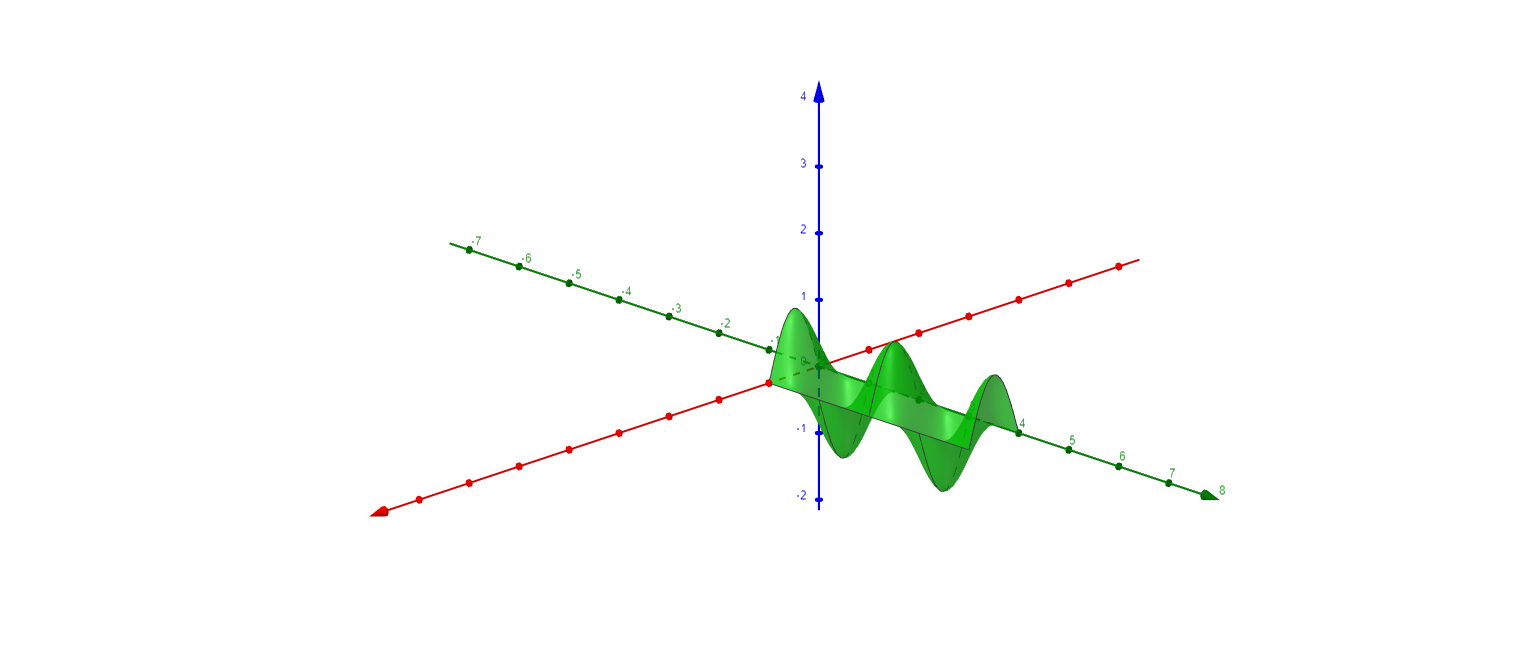
\includegraphics[width=.5\textwidth]{Figures/wave_solution_2.png}
        \end{figure}
        % \begin{figure}[H]
        %     \centering
        %     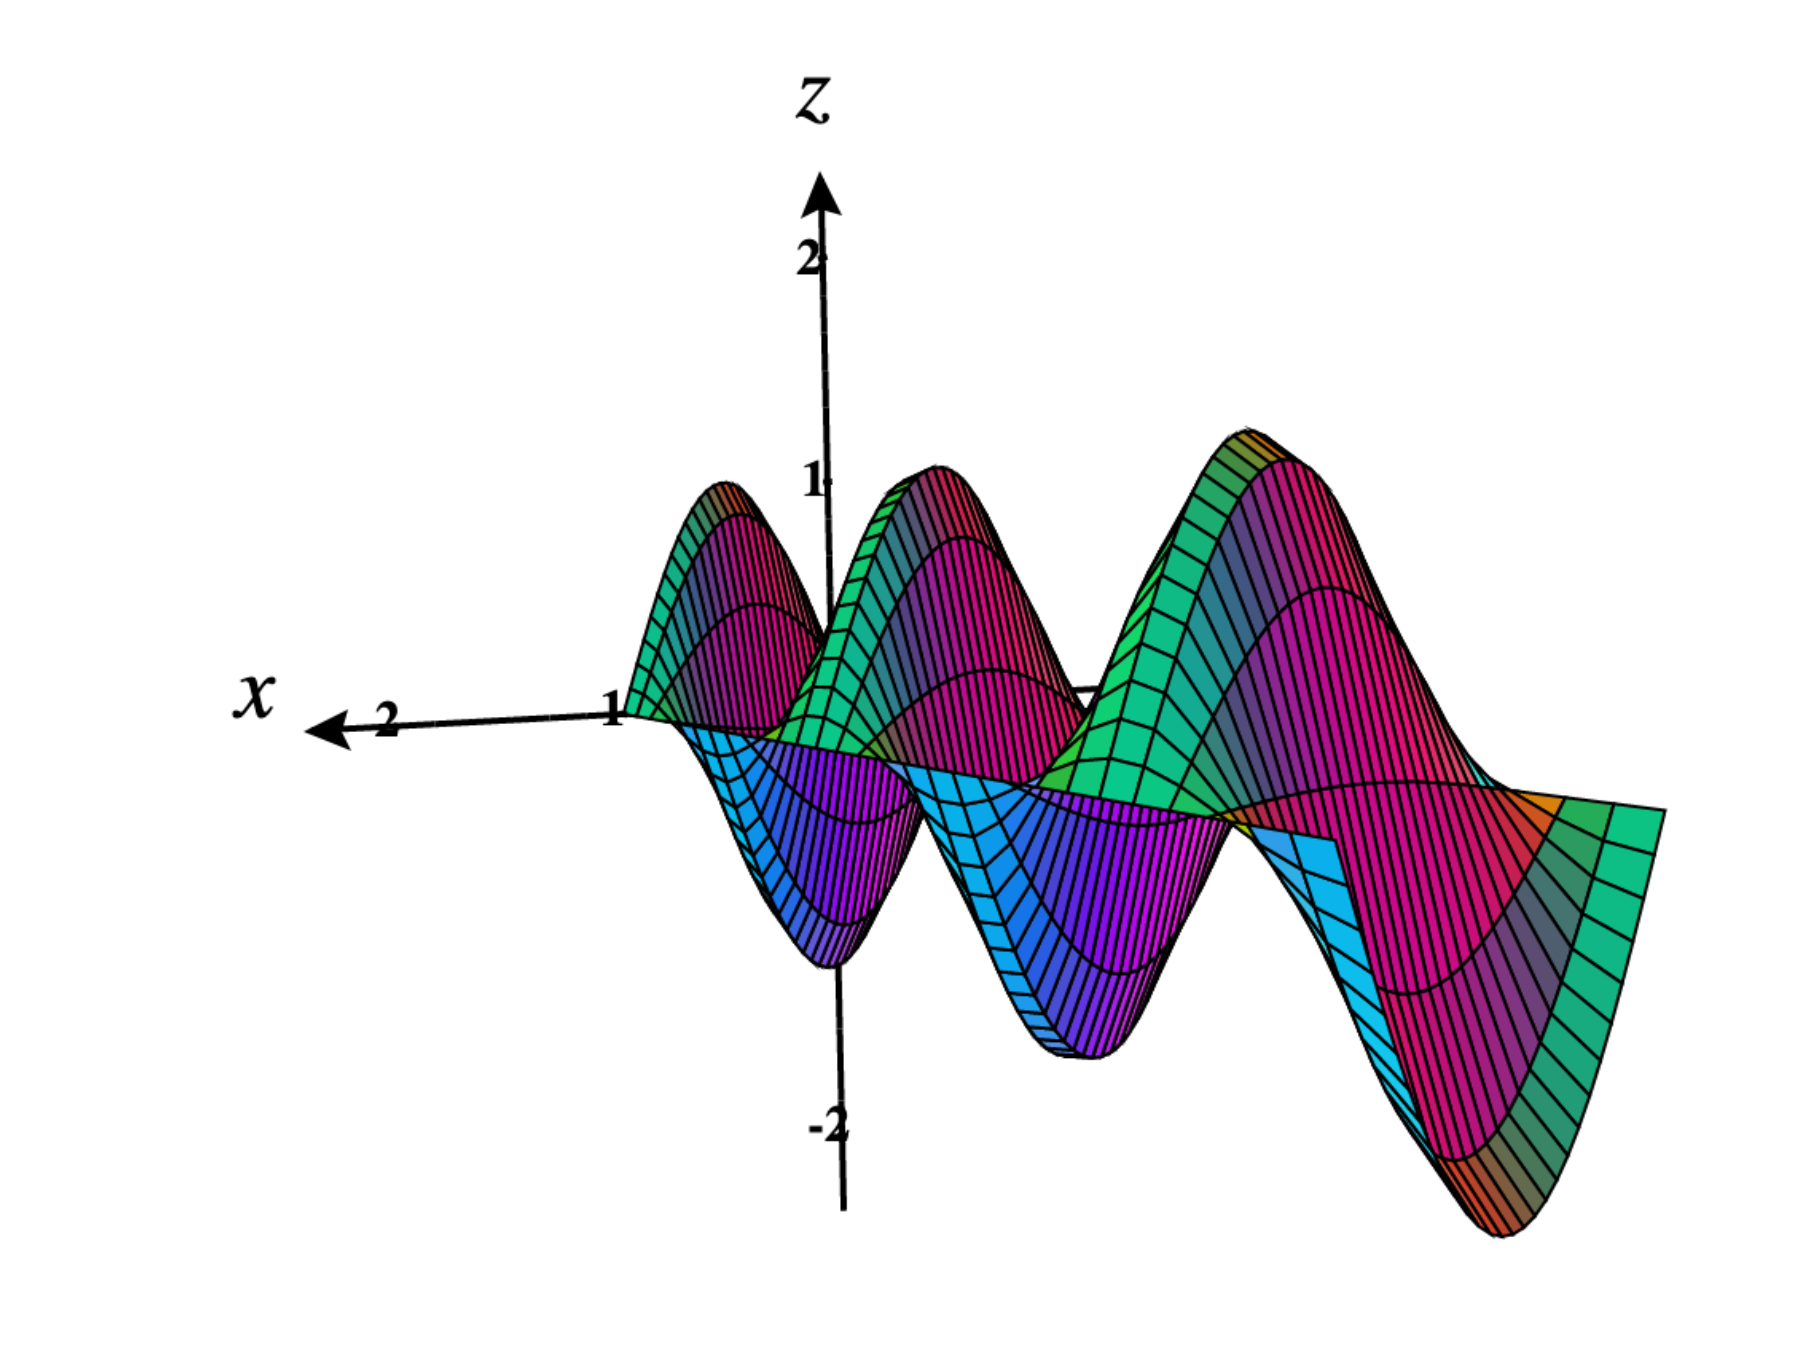
\includegraphics[width=.5\textwidth]{Figures/wave_solution.png}
        % \end{figure}
        \end{ex}

% \end{document}

 

\printindex 

 
\end{document}